\documentclass[11pt,a4paper]{article}

\usepackage[margin=2.5cm]{geometry}
\usepackage{graphicx}
\usepackage{amsmath,amssymb}
\usepackage{booktabs}
\usepackage{hyperref}
\usepackage[font=small,labelfont=bf]{caption}
\usepackage{float}
\usepackage{parskip}

\title{Pheromone Trail Formation at the Edge of Chaos:\\
  Phase Diagrams of a Lattice Ant Model}
\author{}
\date{}

\begin{document}
\maketitle

\begin{abstract}
We study edge-of-chaos dynamics in a lattice ant model where agents deposit pheromone, follow concentration gradients, and explore with directional momentum.
A composite order parameter $C = S \times (1 - A)$---spatial structure times temporal decorrelation---locates the edge of chaos between frozen trail networks and spatial disorder.
Of nine model variants tested, only two produce an edge-of-chaos ridge, and both share the same essential ingredient: uniform pheromone decay.
The minimal system---ants that deposit where they walk, follow concentrations above a threshold, and a field that decays uniformly---produces edge of chaos naturally at the balance point between trail formation and trail erosion.
Seven alternative mechanisms (follow probability, habituation, sensory saturation, Hill function chemoreception, peaked response, coupled deposition) all fail because they introduce disorder that is \emph{correlated} with the pheromone field.
Edge of chaos is the default in stigmergic systems with uniform decay; the hard problem is not producing it but not destroying it.
\end{abstract}

% ================================================================
\section{The Model}
% ================================================================

\subsection{Setup}

Consider $N$ agents (ants) on a $W \times H$ toroidal grid with Moore neighbourhood.
Each cell is either empty or occupied by one ant.
A continuous environment field $\phi(x,y,t) \geq 0$ represents pheromone concentration.

Each ant maintains a heading vector $\mathbf{h} = (h_r, h_c)$, updated as an exponential moving average of recent move directions.

\subsection{Movement rule}

At each time step, every ant attempts to move to an empty neighbouring cell.
The probability of choosing neighbour $j$ is:

\begin{equation}
  p(j) = \frac{w(j)}{\sum_k w(k)}, \qquad
  w(j) = \underbrace{(\beta + \phi_j)^n}_{\text{pheromone attraction}}
         \;\times\;
         \underbrace{\max\!\bigl(0.01,\; 1 + \mu \cos\theta_j\bigr)}_{\text{momentum}}
  \label{eq:weight}
\end{equation}

where $\phi_j$ is the pheromone at cell $j$, $\beta$ is a baseline exploration constant, $n$ is the bias exponent, $\mu$ is the momentum strength, and $\theta_j$ is the angle between the ant's heading $\mathbf{h}$ and the direction to cell $j$.

With probability $\varepsilon$ (the \emph{noise} parameter), the ant ignores both pheromone and momentum, choosing uniformly among empty neighbours.

After each move, the heading is updated:
\begin{equation}
  \mathbf{h} \leftarrow (1 - \alpha)\,\mathbf{h} + \alpha\,\Delta\mathbf{r}
  \label{eq:heading}
\end{equation}
where $\Delta\mathbf{r}$ is the move direction and $\alpha$ is the heading adaptation rate.

\subsection{Pheromone dynamics}

Each ant deposits a fixed amount $\delta$ of pheromone at its current cell every step.
The field then undergoes two global operations:

\begin{align}
  \text{Evaporation:} \quad & \phi \leftarrow (1 - \lambda)\,\phi \label{eq:evap} \\
  \text{Diffusion:}   \quad & \phi \leftarrow \phi + \sigma\,\nabla^2\phi \label{eq:diff}
\end{align}

where $\lambda$ is the evaporation rate and $\sigma$ is the diffusion rate.
The Laplacian $\nabla^2\phi$ is computed as the sum over Moore neighbours minus 8 times the centre value, normalised appropriately.

\subsection{Parameters}

Table~\ref{tab:params} lists the full parameter set.
The first group (topology, ant density, deposition) defines the physical setup.
The second group (movement rule) controls individual ant behaviour.
The third group (field operations) controls the shared pheromone medium.

\begin{table}[H]
\centering
\caption{Model parameters. The two swept parameters are shown in bold.}
\label{tab:params}
\begin{tabular}{@{}llll@{}}
\toprule
Parameter & Symbol & Value & Role \\
\midrule
Grid size & $W \times H$ & $100 \times 100$ & Toroidal lattice \\
Ant density & $\rho$ & 2.5--5\% & Fraction of cells occupied \\
Deposition & $\delta$ & 5.0--6.0 & Pheromone deposited per ant per step \\
\midrule
Bias exponent & $n$ & 2.5--3.0 & Superlinear pheromone preference \\
Bias base & $\beta$ & 0.1--0.3 & Spontaneous exploration baseline \\
Momentum & $\mu$ & 2.0--5.0 & Directional persistence strength \\
Heading rate & $\alpha$ & 0.3--0.4 & EMA smoothing of heading \\
\textbf{Noise} & $\boldsymbol{\varepsilon}$ & \textbf{0.0--0.50} & \textbf{Exploration probability} \\
\midrule
\textbf{Evaporation} & $\boldsymbol{\lambda}$ & \textbf{0.02--0.45} & \textbf{Pheromone decay rate} \\
Diffusion & $\sigma$ & 0.002--0.005 & Pheromone spreading rate \\
\bottomrule
\end{tabular}
\end{table}

% ================================================================
\section{Emergent Trail Formation}
% ================================================================

From uniform random initial placement, ants self-organise into trail networks through positive feedback: deposited pheromone attracts other ants, which deposit more pheromone, reinforcing the trail.
Momentum causes ants to travel \emph{along} trails rather than clustering at high-pheromone spots, producing linear highways rather than blobs.

Figure~\ref{fig:trails} shows trail formation in the equilibrium regime ($\varepsilon = 0$, $\lambda = 0.08$).
By $t = 1000$, a persistent highway network has formed.
Figure~\ref{fig:heatmap} shows the final ant positions alongside the pheromone field, revealing the correspondence between ant traffic and trail structure.

\begin{figure}[H]
\centering
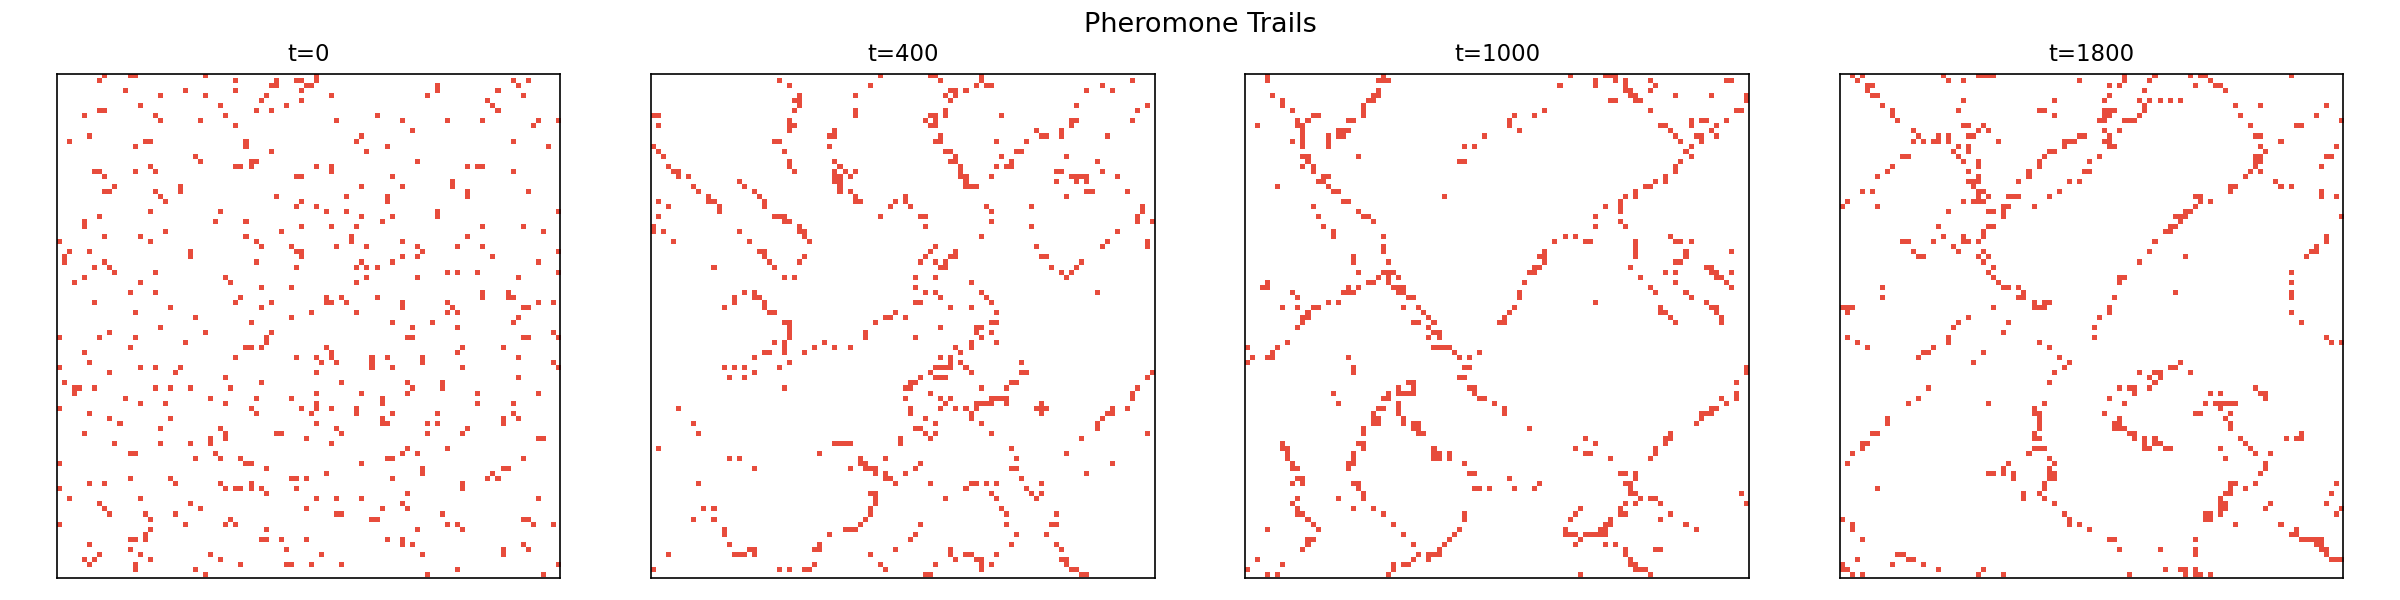
\includegraphics[width=\textwidth]{fig_trails_equil.png}
\caption{Ant positions over time in the equilibrium regime.
  From uniform random placement ($t=0$), ants self-organise into persistent trail networks ($t=1800$).
  Parameters: $n=3$, $\beta=0.1$, $\mu=5$, $\varepsilon=0$, $\lambda=0.08$, $\sigma=0.002$.}
\label{fig:trails}
\end{figure}

\begin{figure}[H]
\centering
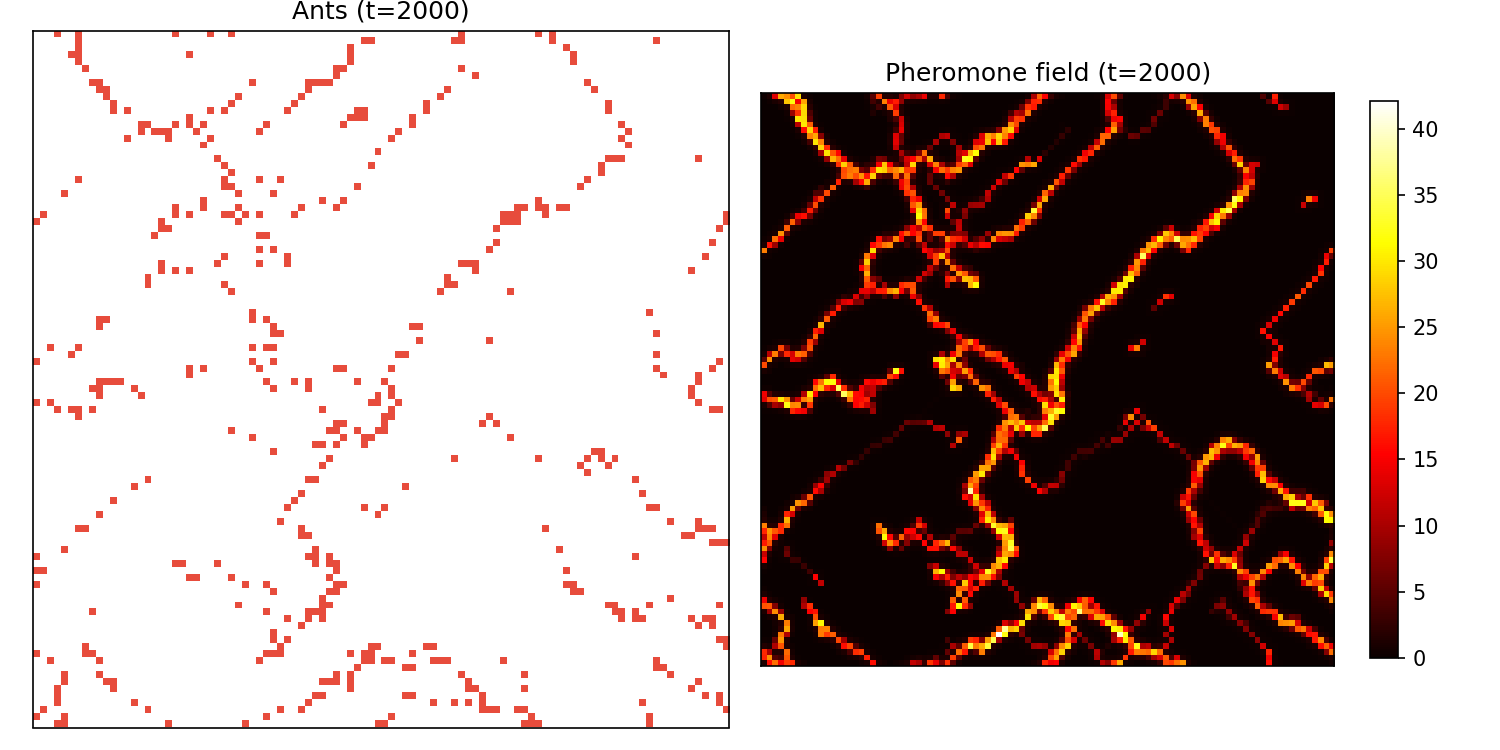
\includegraphics[width=0.85\textwidth]{fig_heatmap.png}
\caption{Equilibrium state at $t=2000$.
  Left: ant positions. Right: pheromone field intensity.
  The trail network is a self-reinforcing structure maintained by ant traffic.}
\label{fig:heatmap}
\end{figure}

In the transient regime ($\varepsilon = 0.10$, $\lambda = 0.12$), trails form but continuously reorganise (Figure~\ref{fig:transient}).
This is the edge-of-chaos regime: structured but impermanent.

\begin{figure}[H]
\centering
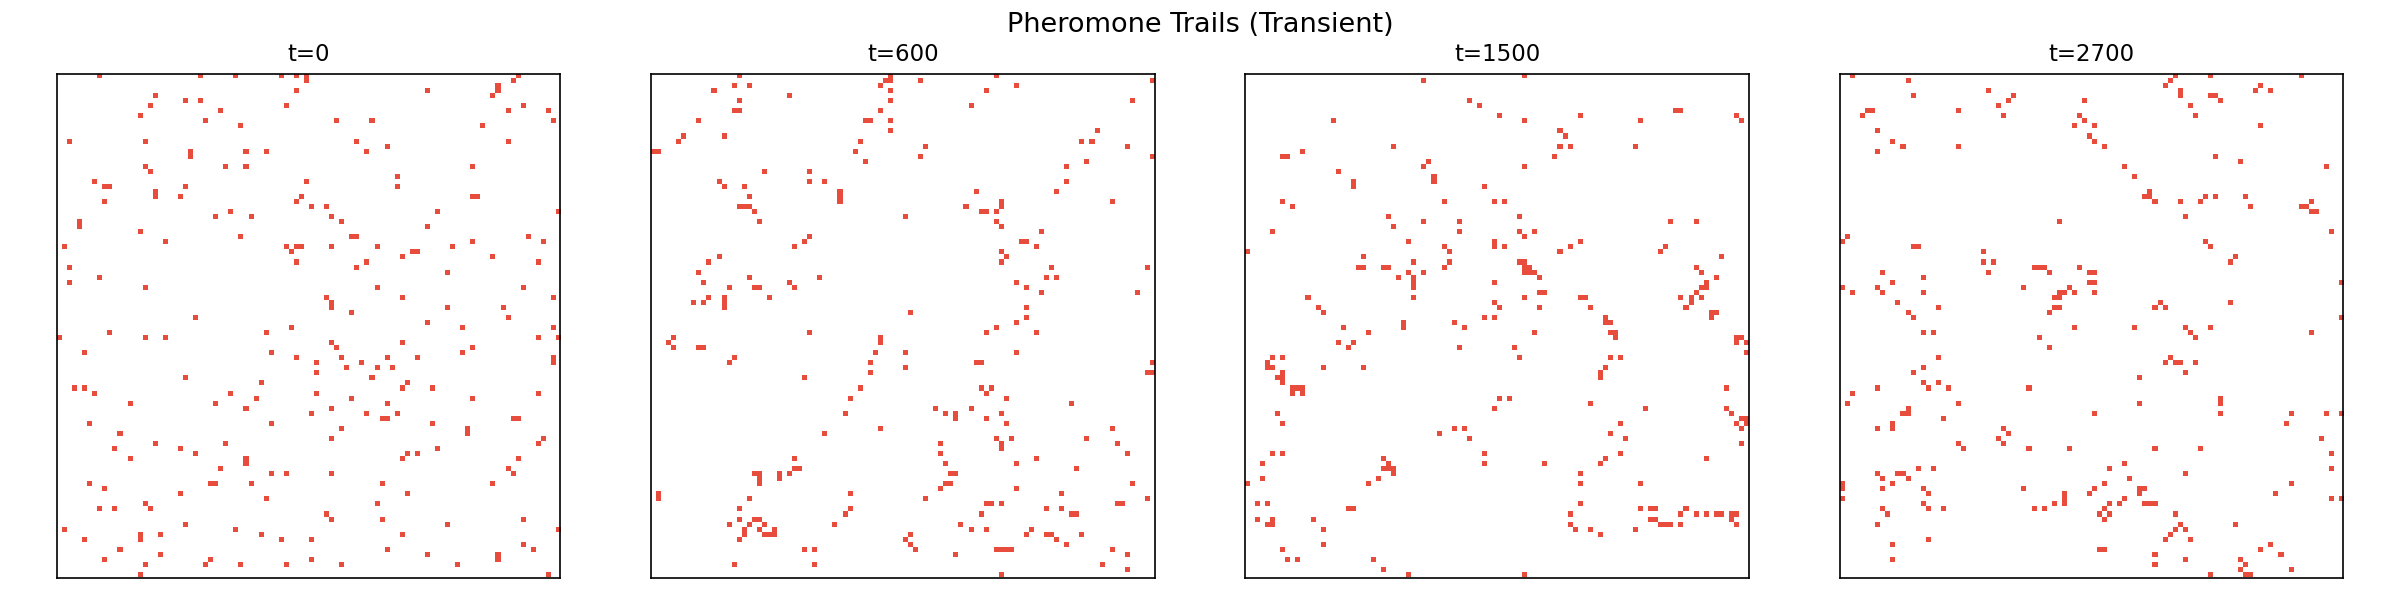
\includegraphics[width=\textwidth]{fig_trails_transient.png}
\caption{Transient regime: trails form and dissolve over time.
  The trail network at $t=600$ differs from the network at $t=2700$.
  Parameters: $n=2.5$, $\beta=0.3$, $\mu=2$, $\varepsilon=0.10$, $\lambda=0.12$, $\sigma=0.003$.}
\label{fig:transient}
\end{figure}

% ================================================================
\section{Order Parameters}
% ================================================================

To locate the edge of chaos, we need scalar quantities that distinguish the three regimes.

\subsection{Field autocorrelation}

The Pearson correlation between the pheromone field at times $t$ and $t - \tau$:
\begin{equation}
  A(\tau) = \frac{\sum_{x,y} (\phi_{t} - \bar\phi_{t})(\phi_{t-\tau} - \bar\phi_{t-\tau})}
                 {\sqrt{\sum(\phi_{t} - \bar\phi_{t})^2} \sqrt{\sum(\phi_{t-\tau} - \bar\phi_{t-\tau})^2}}
  \label{eq:autocorr}
\end{equation}

This measures trail persistence: $A \approx 1$ for frozen trails, $A \approx 0$ for transient or disordered states.
It distinguishes frozen from non-frozen but cannot distinguish ``different trails'' from ``no trails''---both give low autocorrelation.

\subsection{Trail linearity}

Define ``hot'' cells as those where $\phi > 0.3 \cdot \max(\phi)$.
Trail linearity is the fraction of hot cells with exactly 2 hot Moore neighbours:
\begin{equation}
  L = \frac{|\{(x,y) : \text{hot}(x,y) \;\wedge\; |\mathcal{N}_{\text{hot}}(x,y)| = 2\}|}{|\{(x,y) : \text{hot}(x,y)\}|}
  \label{eq:linearity}
\end{equation}

Cells with exactly 2 hot neighbours form \emph{chains}---the topological signature of a trail.
Cells with many hot neighbours are blob-like; cells with 0--1 are isolated.
High linearity indicates trail-like structure regardless of whether those trails persist over time.

\subsection{The linearity metric and its limitations}
\label{sec:linearity-problem}

Trail linearity was our initial structure metric and is used in the original and simple model sweeps (Sections 4--5).
However, it has a fundamental limitation: it cannot distinguish trail structure produced by \emph{collective following} from spatial texture produced by \emph{individual momentum}.

When ants deposit pheromone while walking with directional persistence ($\mu > 0$), evaporation sculpts the deposition pattern into a landscape of hot spots.
Some of these spots will randomly have exactly 2 hot Moore neighbours---scoring as ``trail-like''---even though no trail-following behaviour produced them.
This creates a linearity floor of $L \approx 0.20$--$0.30$ regardless of whether ants are following pheromone or walking independently.

In a metric comparison across susceptibility regimes (Section~\ref{sec:susceptibility}), linearity varied by only $\sim$10\% between full trail-following ($\text{ff} = 1.0$, $L = 0.25$) and zero following ($\text{ff} = 0$, $L = 0.23$).
The metric is essentially blind to the collective dynamics we are trying to measure.

\subsection{Block variance: a statistical alternative}

To replace linearity, we need a metric that captures spatial structure at a scale larger than individual cells.
Trail networks create \emph{mesoscale heterogeneity}: some regions of the grid contain highways with concentrated pheromone, while others are empty corridors.
Random deposition from individually moving ants creates cell-level texture but is approximately uniform at the mesoscale.

We divide the $W \times H$ grid into non-overlapping blocks of size $b \times b$ and compute the mean pheromone in each block.
The block variance is the normalised variance of these block means:
\begin{equation}
  B = \frac{\text{Var}(\bar\phi_{\text{blocks}})}{\bar\phi^2}
  \label{eq:block_variance}
\end{equation}
where $\bar\phi_{\text{blocks}}$ is the vector of block-averaged pheromone values and $\bar\phi$ is the global mean.
Dividing by $\bar\phi^2$ makes the metric scale-invariant with respect to overall pheromone intensity.

Block variance is high when pheromone is concentrated in certain regions (trail networks) and low when it is spread uniformly (random deposition).
In our metric comparison, block variance dropped by $\sim$50\% between the following and non-following regimes---far more discriminating than linearity's $\sim$10\%.

\subsection{Composite order parameter}

Neither observable alone peaks at the edge of chaos.
Autocorrelation is high in the frozen regime and low everywhere else.
The structure metric (linearity $L$ or block variance $B$) is high in the frozen and transient regimes.
We construct:
\begin{equation}
  C = S \times (1 - A)
  \label{eq:composite}
\end{equation}
where $S$ is the structure metric ($L$ for the original and simple models, $B$ for the susceptibility model).

This is maximised where trails \emph{exist} ($S > 0$) but are \emph{transient} ($A < 1$), and is zero in two failure modes: no trails ($S = 0$) or frozen trails ($A = 1$).
The product is structurally similar to the LMC statistical complexity $C_{\text{LMC}} = H \times D$ of L\'opez-Ruiz, Mancini \& Calbet (1995), where our structure metric $S$ plays the role of disequilibrium $D$ (spatial order) and $(1-A)$ plays the role of entropy $H$ (temporal disorder).

% ================================================================
\section{Phase Diagram: The Original Model}
% ================================================================

We swept noise $\varepsilon \in [0, 0.50]$ and evaporation $\lambda \in [0.02, 0.45]$ on a $13 \times 13$ grid (169 simulations), each running 600 steps on a $60 \times 60$ grid with $\rho = 3.75\%$.
All other parameters were held fixed at $n = 2.5$, $\beta = 0.3$, $\mu = 2.0$, $\alpha = 0.4$, $\delta = 6.0$, $\sigma = 0.005$.

\begin{figure}[H]
\centering
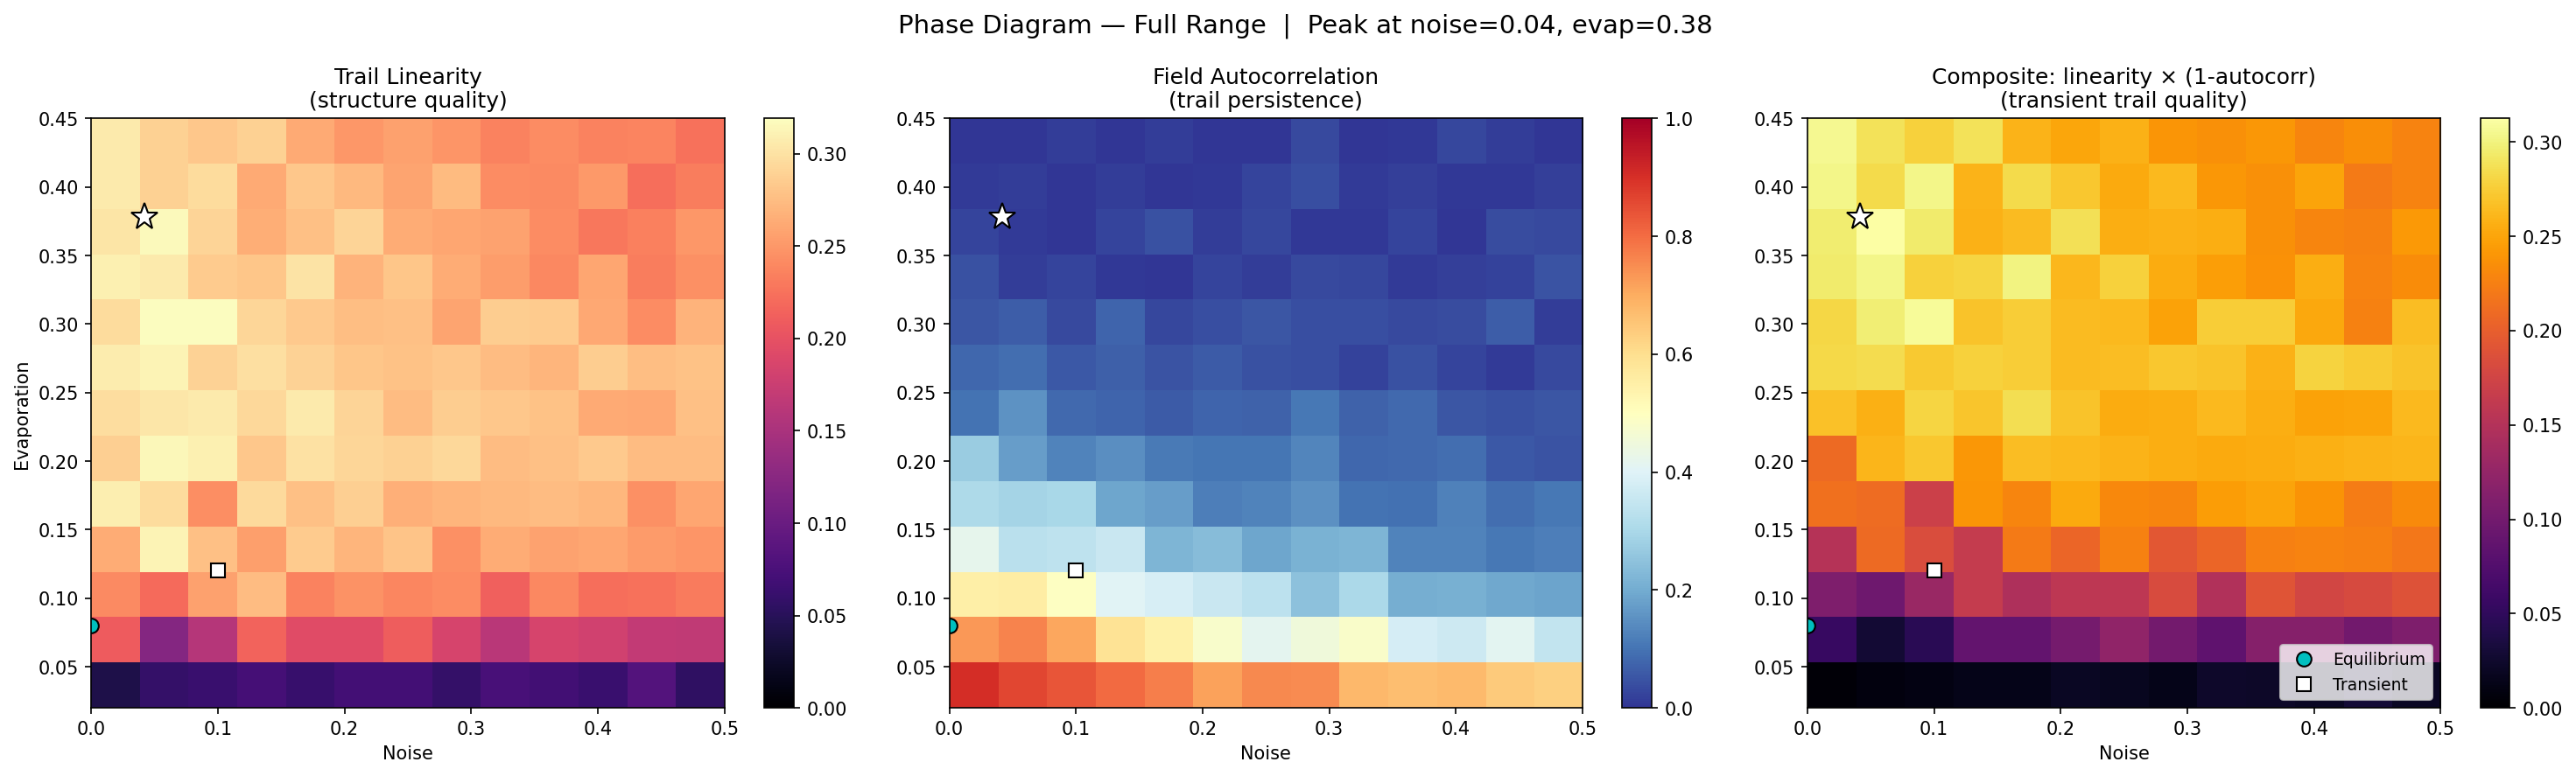
\includegraphics[width=\textwidth]{fig_triptych_original.png}
\caption{Phase diagram of the original model.
  Left: trail linearity. Centre: field autocorrelation. Right: composite $C = L \times (1 - A)$.
  Star marks the composite peak ($\varepsilon = 0.04$, $\lambda = 0.38$, $C = 0.312$).
  Circle: equilibrium spec. Square: transient spec.}
\label{fig:triptych_original}
\end{figure}

The phase diagram (Figure~\ref{fig:triptych_original}) reveals three regimes:

\begin{itemize}
  \item \textbf{Frozen trails} (bottom strip, $\lambda < 0.10$): Persistent highway networks. Autocorrelation $A > 0.5$. The composite is low because $(1 - A) \approx 0$.
  \item \textbf{Transient trails} (middle-to-upper band): Trails form but rewire. Autocorrelation $A \in [0.05, 0.3]$. Linearity remains high. The composite peaks here.
  \item \textbf{Disorder} (top-right, high $\varepsilon$ and $\lambda$): No coherent structure. Both $L$ and $A$ are low.
\end{itemize}

The composite peak at $\varepsilon = 0.04$, $\lambda = 0.38$ reveals that the edge of chaos has very low noise (ants are mostly deterministic followers) and very high evaporation (the environment rapidly erases trails).
The non-equilibrium regime is driven by \emph{environmental erasure} rather than \emph{behavioural randomness}.

\begin{figure}[H]
\centering
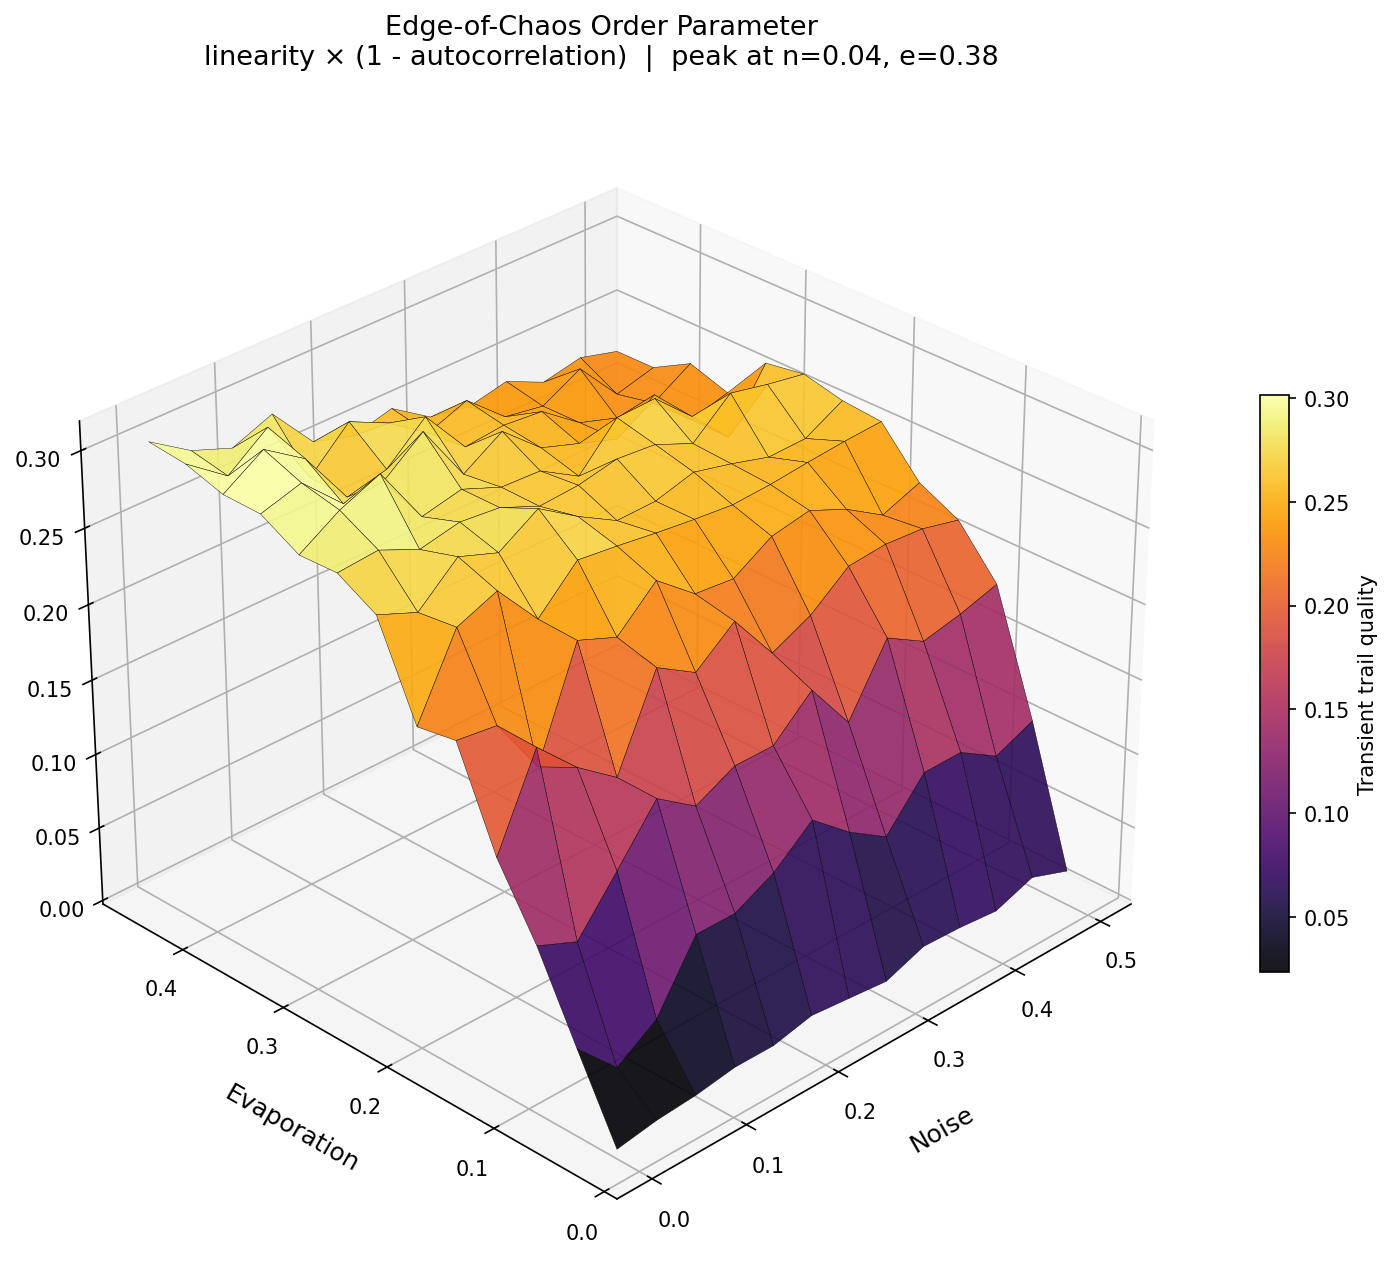
\includegraphics[width=0.6\textwidth]{fig_surface_original.png}
\caption{3D surface of the composite order parameter.
  The ridge runs along low noise at moderate-to-high evaporation.
  It drops to zero in two directions: downward (trails freeze) and rightward (structure destroyed by noise).}
\label{fig:surface_original}
\end{figure}

The composite surface (Figure~\ref{fig:surface_original}) forms a ridge, not a peak---it extends along the evaporation axis, reflecting the asymmetry between the two disruption mechanisms.
Evaporation destroys trail \emph{persistence} without destroying trail \emph{structure}; noise destroys both.

\subsection{Regimes across parameter space}

Figures~\ref{fig:snapshot_phero} and~\ref{fig:snapshot_ants} show the pheromone fields and ant positions at representative points across the noise--evaporation plane.
Reading left to right (increasing noise) shows the transition from frozen highways to disorder.
Reading bottom to top (increasing evaporation) shows trails becoming more transient and eventually dissolving.
The edge-of-chaos regime---visible as bright, structured trails with moderate ant clustering---occupies a diagonal band from low noise / high evaporation to moderate noise / low evaporation.

\begin{figure}[H]
\centering
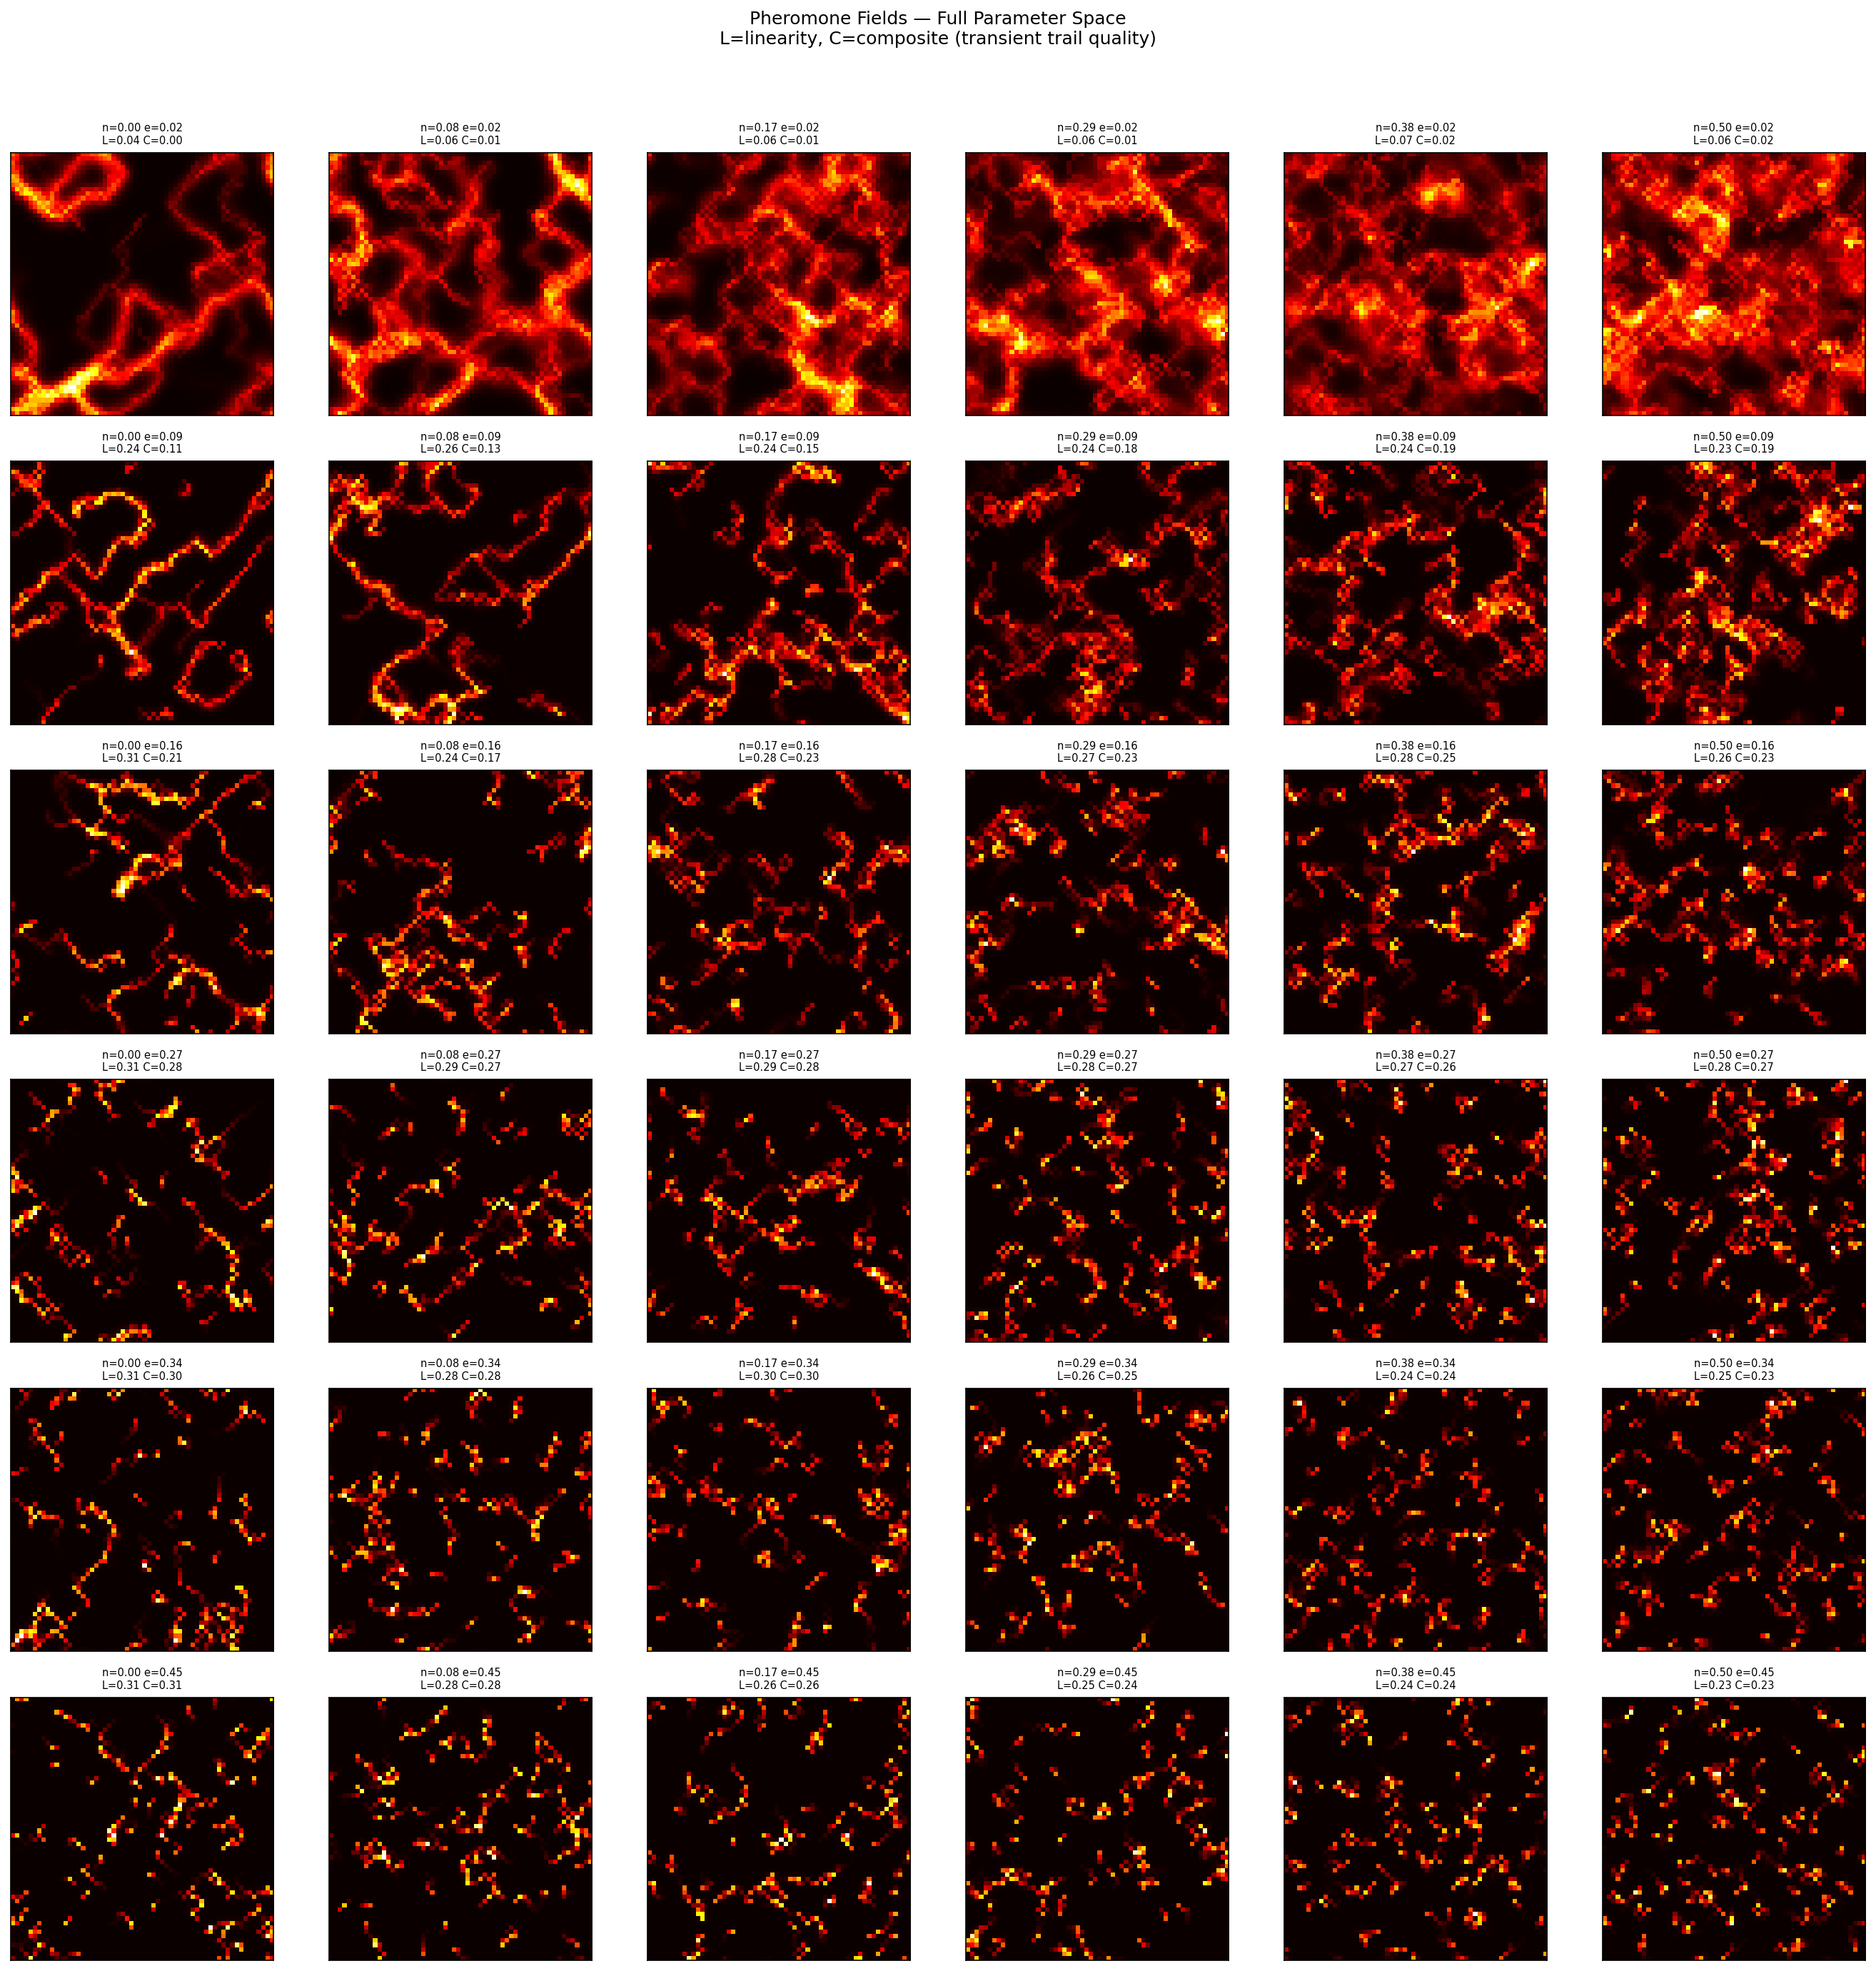
\includegraphics[width=\textwidth]{snapshot_grid_full.png}
\caption{Pheromone fields across the noise--evaporation parameter space.
  Rows increase in evaporation (bottom to top); columns increase in noise (left to right).
  Bottom-left: frozen trail networks with high pheromone concentration.
  Top-right: spatial disorder with no coherent structure.
  The diagonal band between these extremes shows transient trails---the edge of chaos.
  L = linearity, C = composite order parameter.}
\label{fig:snapshot_phero}
\end{figure}

\begin{figure}[H]
\centering
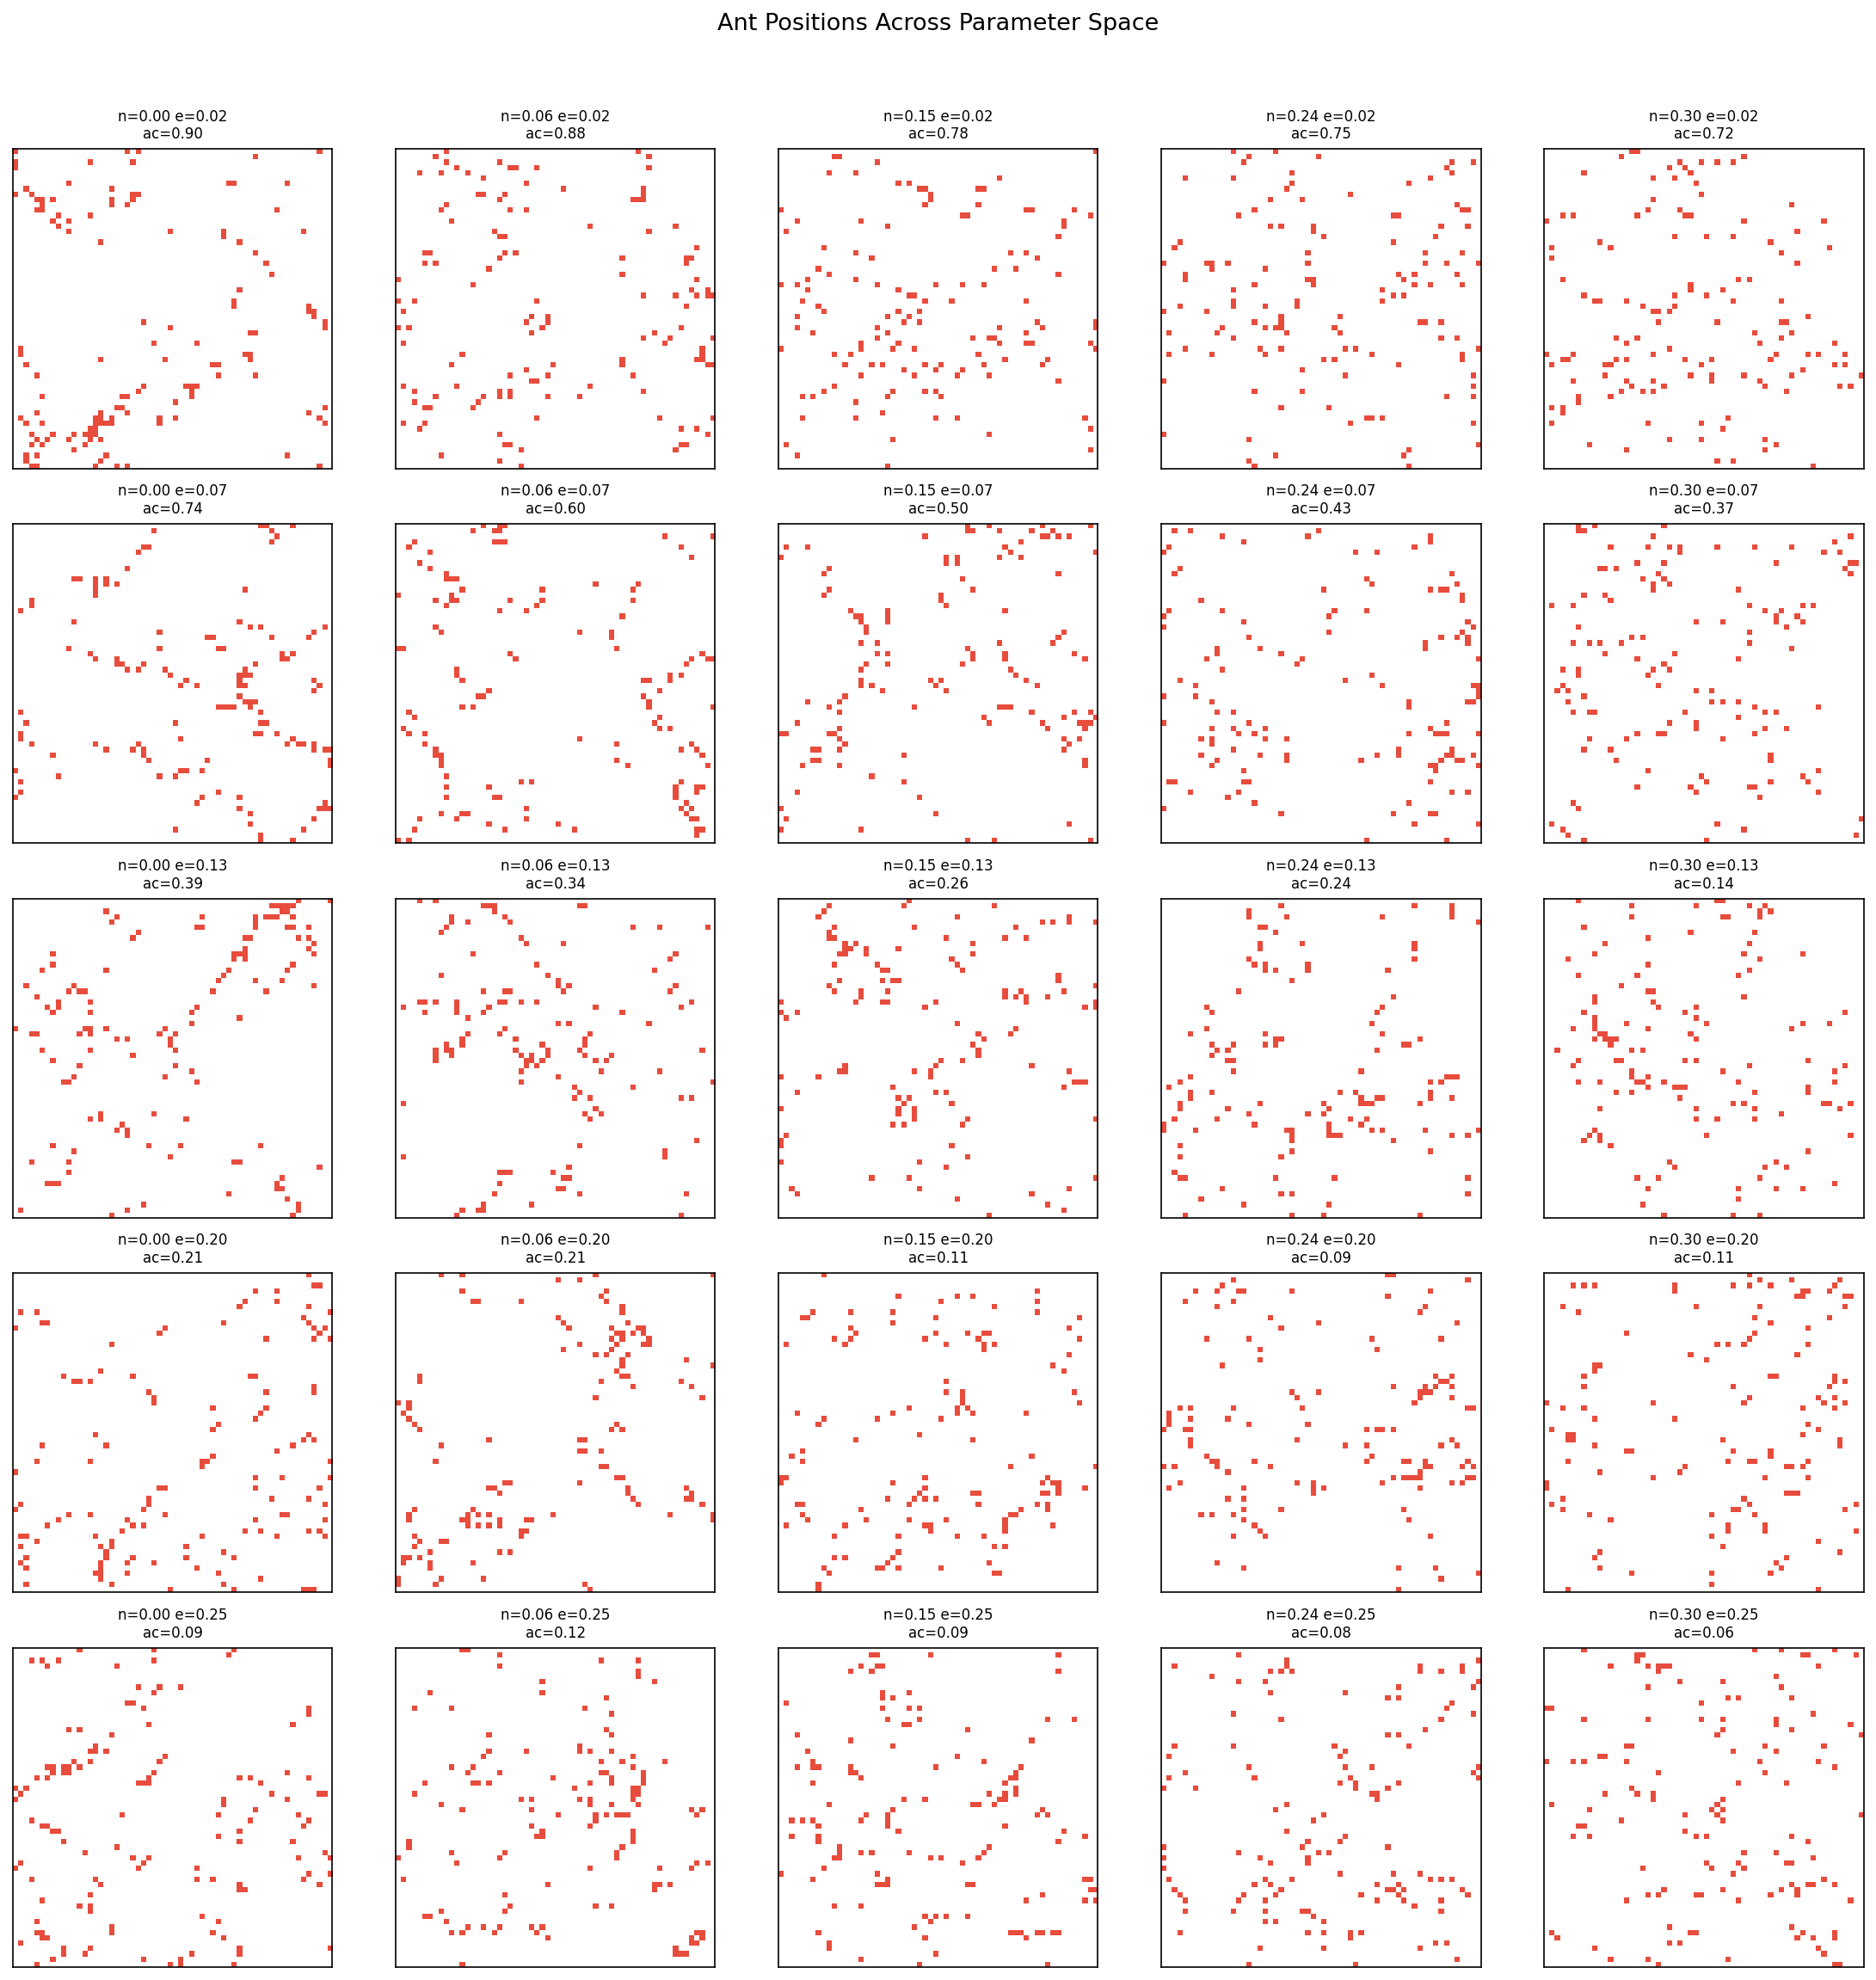
\includegraphics[width=\textwidth]{snapshot_grid_ants.png}
\caption{Ant positions corresponding to Figure~\ref{fig:snapshot_phero}.
  In the frozen regime (bottom-left), ants cluster tightly along persistent trail networks.
  In the transient regime (middle), ants form loose linear aggregations.
  In the disordered regime (top-right), ants are uniformly scattered with no spatial structure.}
\label{fig:snapshot_ants}
\end{figure}

% ================================================================
\section{The Simple Model: Can We Do Without Noise?}
\label{sec:simple}
% ================================================================

\subsection{Motivation}

The noise parameter $\varepsilon$ is a brute-force intervention: with probability $\varepsilon$, the ant ignores \emph{everything}---pheromone, momentum, heading---and moves to a uniformly random neighbour.
This is not a behavioural description.
No real ant has a subroutine that occasionally overwrites its entire decision-making with uniform randomness.

We wanted a model where an individual ant has a simple, coherent behaviour---walk with gentle persistence, occasionally respond to a chemical signal---and complexity emerges purely from social interaction through the pheromone medium.
The individual should be boring; the collective should be complex.

\subsection{Formulation}

Replace the six-parameter movement rule~\eqref{eq:weight} with a coin flip:

\begin{equation}
  \text{Each step:} \quad
  \begin{cases}
    \text{with probability } p_f: & \text{pick neighbour weighted linearly by } \phi_j + 0.01 \\
    \text{otherwise:} & \text{move randomly with momentum } \mu
  \end{cases}
  \label{eq:simple}
\end{equation}

When following pheromone, the weighting is linear (no exponent $n$, no baseline $\beta$).
When not following, the ant walks with its intrinsic momentum---it tends to keep going in its current direction, like a real ant exploring.

This gives three parameters:

\begin{table}[H]
\centering
\caption{Simple model parameters.}
\label{tab:simple}
\begin{tabular}{@{}lll@{}}
\toprule
Parameter & Symbol & Role \\
\midrule
Follow probability & $p_f$ & How often an ant reads the social signal \\
Evaporation & $\lambda$ & How fast the shared memory decays \\
Diffusion & $\sigma$ & How far the signal spreads spatially \\
\bottomrule
\end{tabular}
\end{table}

Momentum $\mu$ and heading rate $\alpha$ are structural constants---properties of ant locomotion, not parameters of the information system.

\subsection{Sweep results: high momentum ($\mu = 3.0$)}

We swept $p_f \in [0, 1]$ and $\lambda \in [0.02, 0.45]$ with $\sigma = 0.005$ fixed.

\begin{figure}[H]
\centering
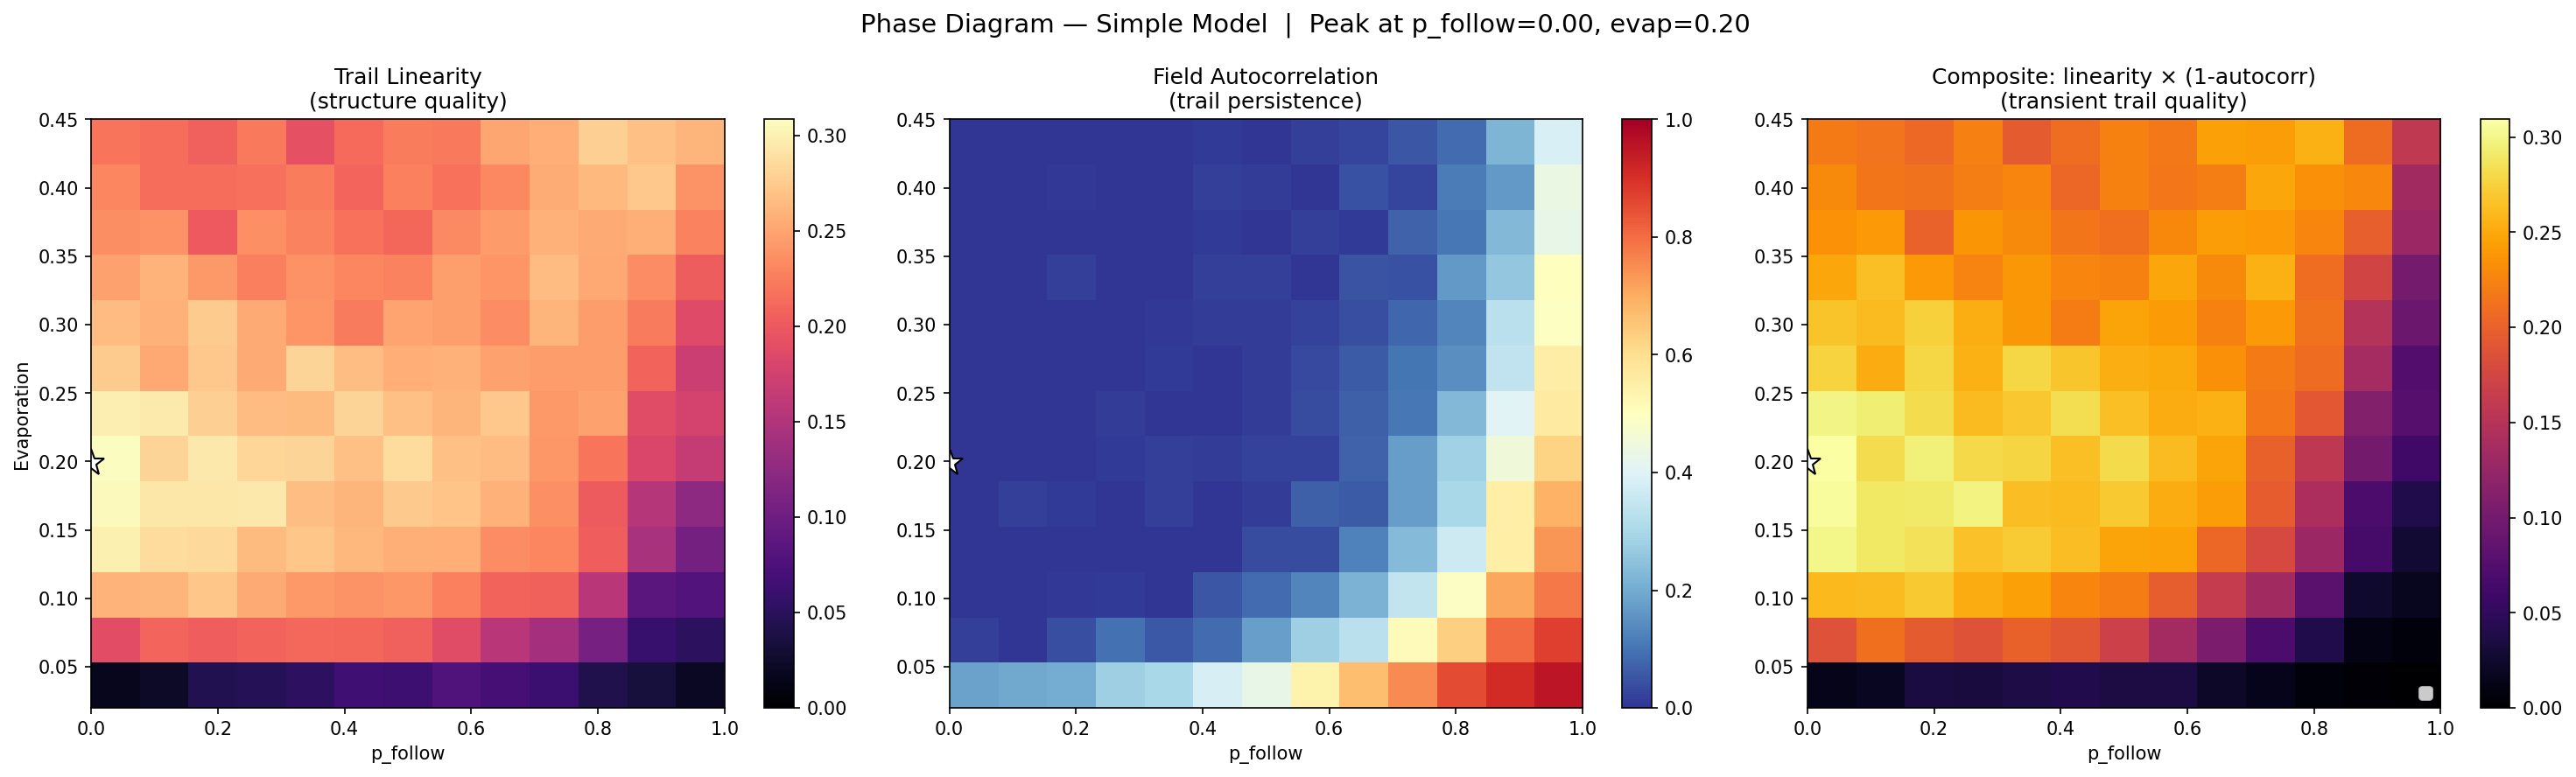
\includegraphics[width=\textwidth]{fig_triptych_simple_highmom.png}
\caption{Phase diagram of the simple model with momentum $\mu = 3.0$.
  The composite peaks at the corner: $p_f = 0$, $\lambda = 0.20$, $C = 0.309$.
  There is no interior peak---no edge of chaos.}
\label{fig:simple_highmom}
\end{figure}

The composite peaks at $p_f = 0$ (Figure~\ref{fig:simple_highmom})---meaning the ``best'' transient trails come from ants that \emph{never follow pheromone}.
This is a boundary artifact, not an edge of chaos.

The problem: with $\mu = 3.0$, the momentum term in the non-following branch weights forward movement $4\times$ vs sideways and $\sim 300\times$ vs backward.
Ants walk in near-straight lines, creating stream-like spatial structure without any pheromone feedback.
The linearity metric saturates at $L \approx 0.30$ regardless of $p_f$.

\textbf{The fundamental asymmetry}: The original model's noise $\varepsilon$ destroys both pheromone following \emph{and} momentum simultaneously.
The simple model's $p_f$ only controls the pheromone signal while leaving momentum intact.
There is no disorder regime---you cannot reach $L = 0$ by adjusting $p_f$ alone when momentum creates order on its own.

\subsection{Low momentum ($\mu = 0.5$): the fix}

At $\mu = 0.5$, forward movement is only $1.5\times$ vs sideways.
Ants meander gently---not Brownian, but not streaming.

\begin{figure}[H]
\centering
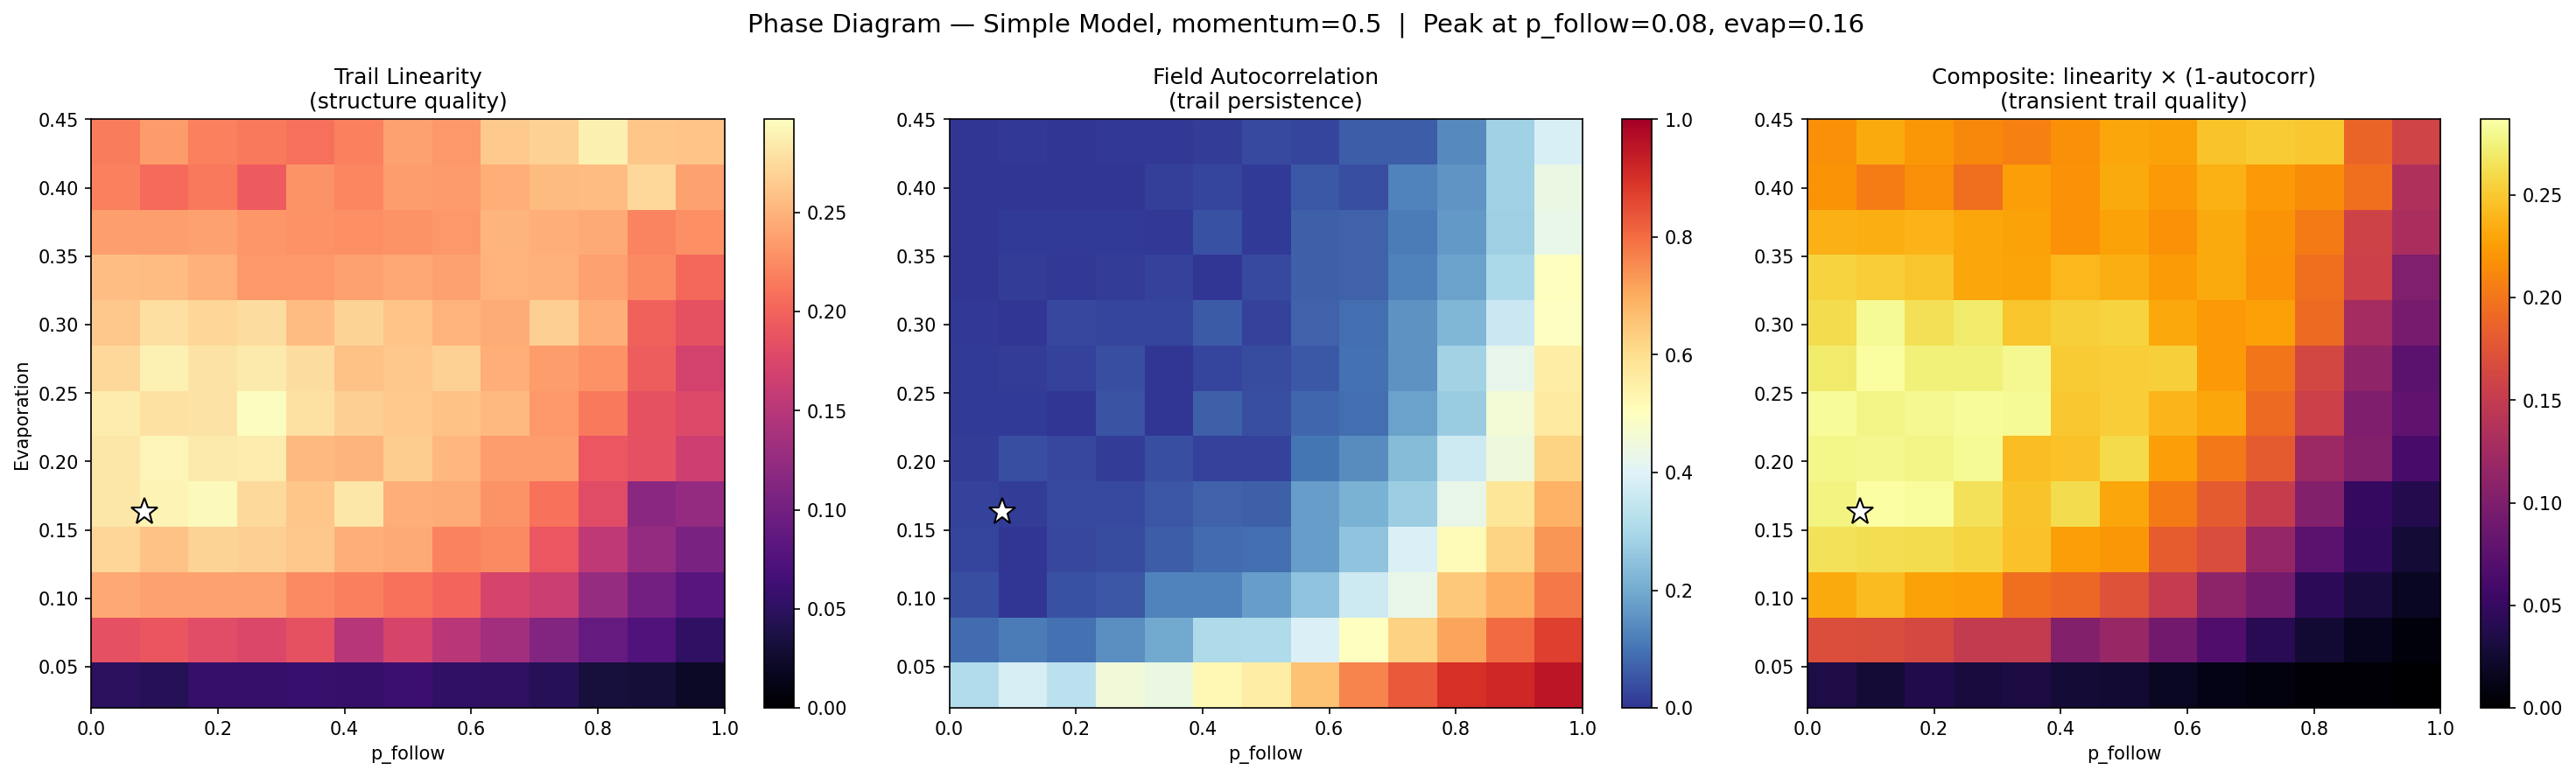
\includegraphics[width=\textwidth]{fig_triptych_simple_lowmom.png}
\caption{Phase diagram of the simple model with momentum $\mu = 0.5$.
  The composite peak moves to the interior: $p_f = 0.08$, $\lambda = 0.16$, $C = 0.287$.}
\label{fig:simple_lowmom}
\end{figure}

\begin{figure}[H]
\centering
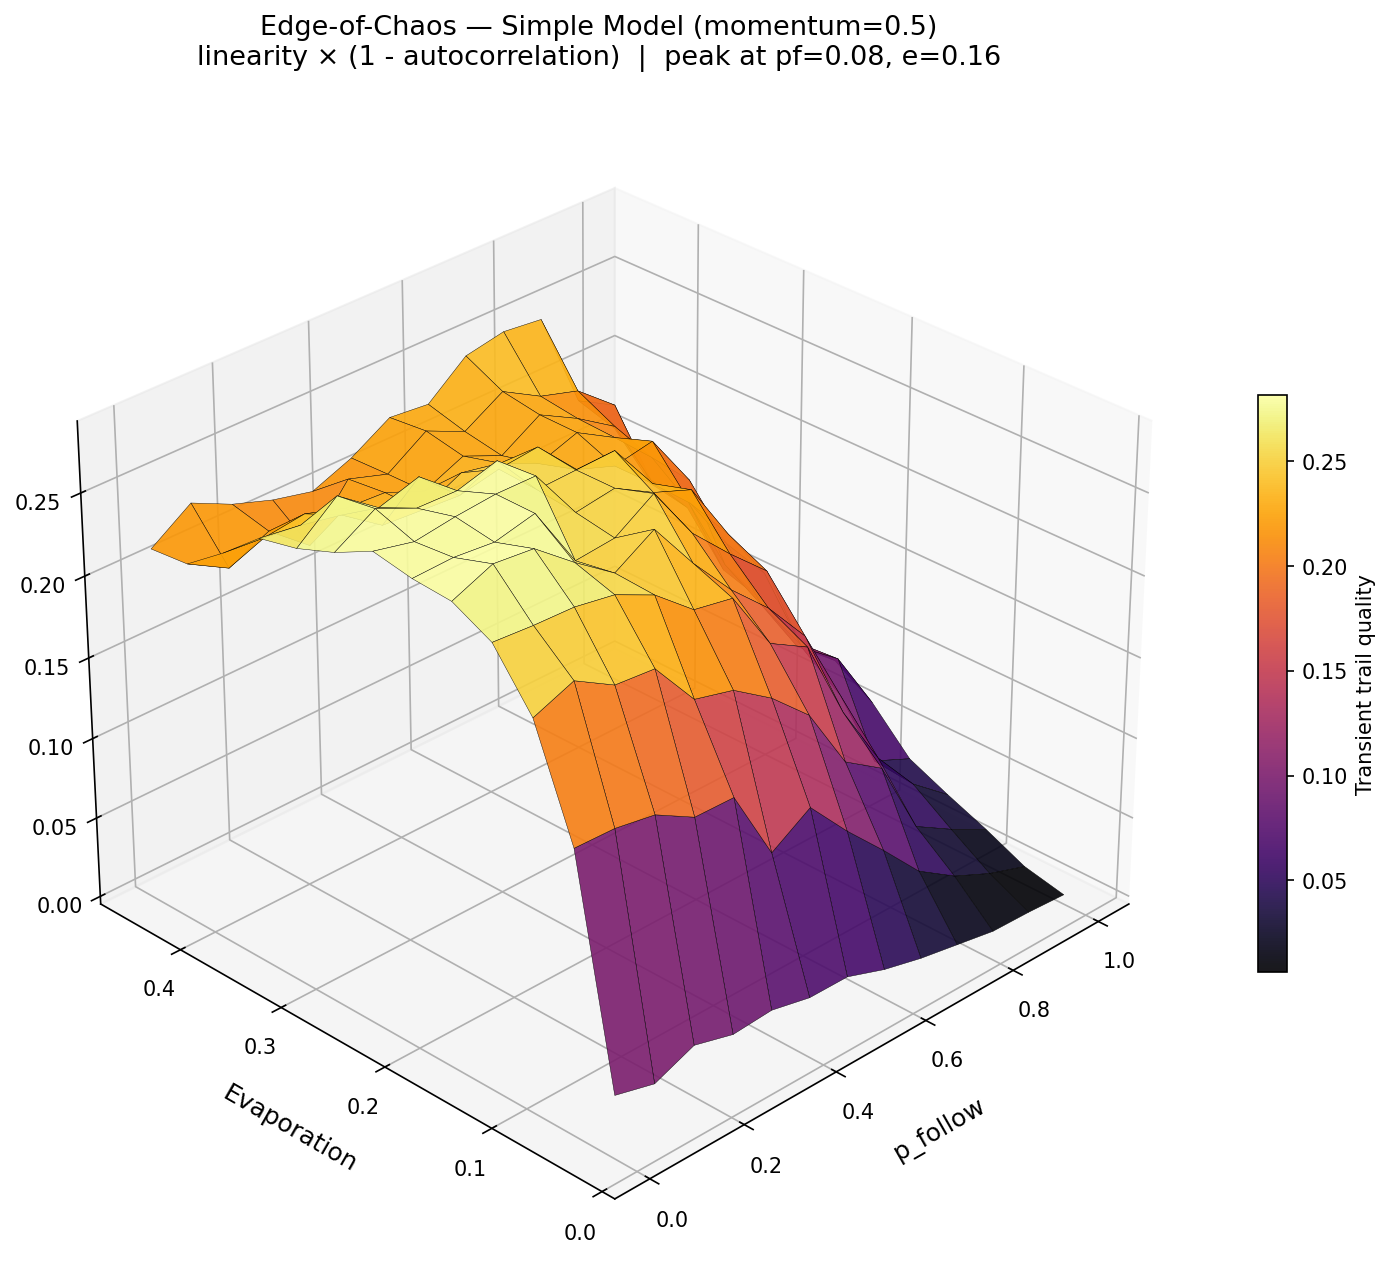
\includegraphics[width=0.6\textwidth]{fig_surface_simple_lowmom.png}
\caption{Composite surface for the simple model at $\mu = 0.5$.
  A shallow hill appears, but the peak is pressed against the $p_f = 0$ edge.}
\label{fig:surface_simple}
\end{figure}

The composite now has an interior peak at $p_f = 0.08$, $\lambda = 0.16$ (Figures~\ref{fig:simple_lowmom}--\ref{fig:surface_simple}).
But the peak is pressed hard against the boundary---$p_f = 0.08$ means ants follow pheromone only 8\% of the time.

The linearity floor at $p_f = 0$ dropped from $\sim 0.30$ (at $\mu = 3.0$) to $\sim 0.24$, but this is still high enough that the composite is dominated by the autocorrelation factor.

\subsection{Diffusion as the third axis}

We swept all three parameters: $p_f \times \lambda \times \sigma$ in a $9 \times 8 \times 7$ grid (504 simulations) at $\mu = 0.5$.

\begin{figure}[H]
\centering
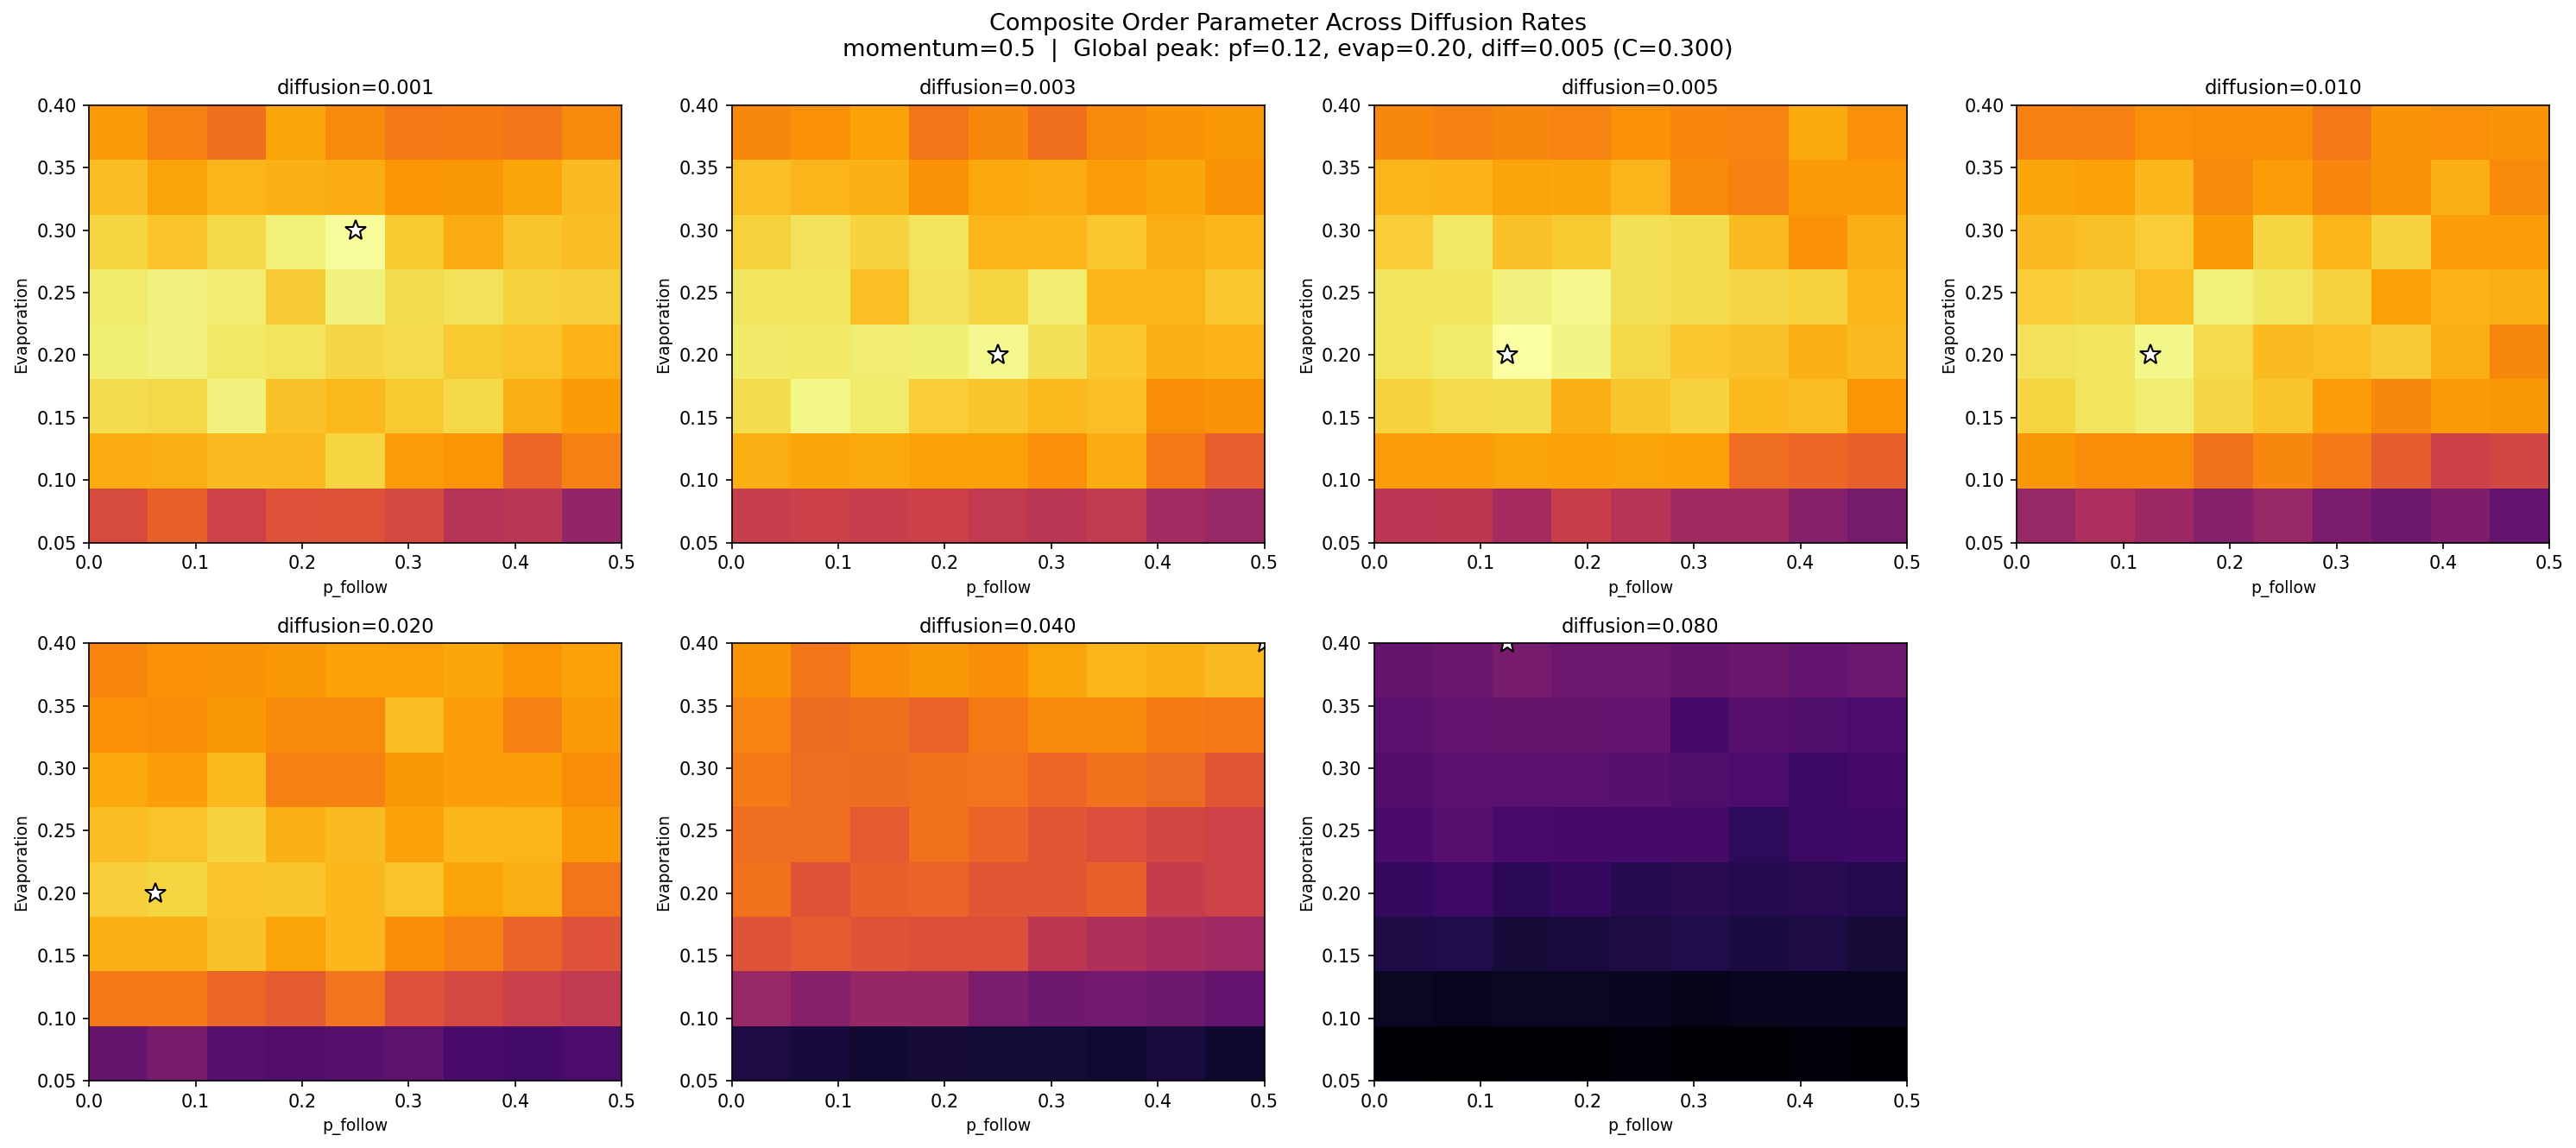
\includegraphics[width=\textwidth]{fig_diffusion_composite.png}
\caption{Composite heatmaps at each diffusion level.
  Stars mark the peak within each slice.
  Global peak: $p_f = 0.12$, $\lambda = 0.20$, $\sigma = 0.005$, $C = 0.300$.
  At $\sigma = 0.08$, pheromone smears into fog and linearity collapses.}
\label{fig:diffusion}
\end{figure}

The global peak sits at $p_f = 0.12$, $\lambda = 0.20$, $\sigma = 0.005$ ($C = 0.300$).
Diffusion controls the spatial scale of the pheromone signal:

\begin{itemize}
  \item \textbf{Too low} ($\sigma < 0.003$): pixel-thin trails; ants must be directly on them to detect pheromone.
    Higher $p_f$ needed to compensate.
  \item \textbf{Optimal} ($\sigma \approx 0.005$): trails create a detectable gradient $\sim$2 cells wide.
    The ant's effective ``sensing range.''
  \item \textbf{Too high} ($\sigma > 0.04$): trails blur into a uniform haze; linearity collapses to $L \approx 0.08$.
\end{itemize}

\begin{figure}[H]
\centering
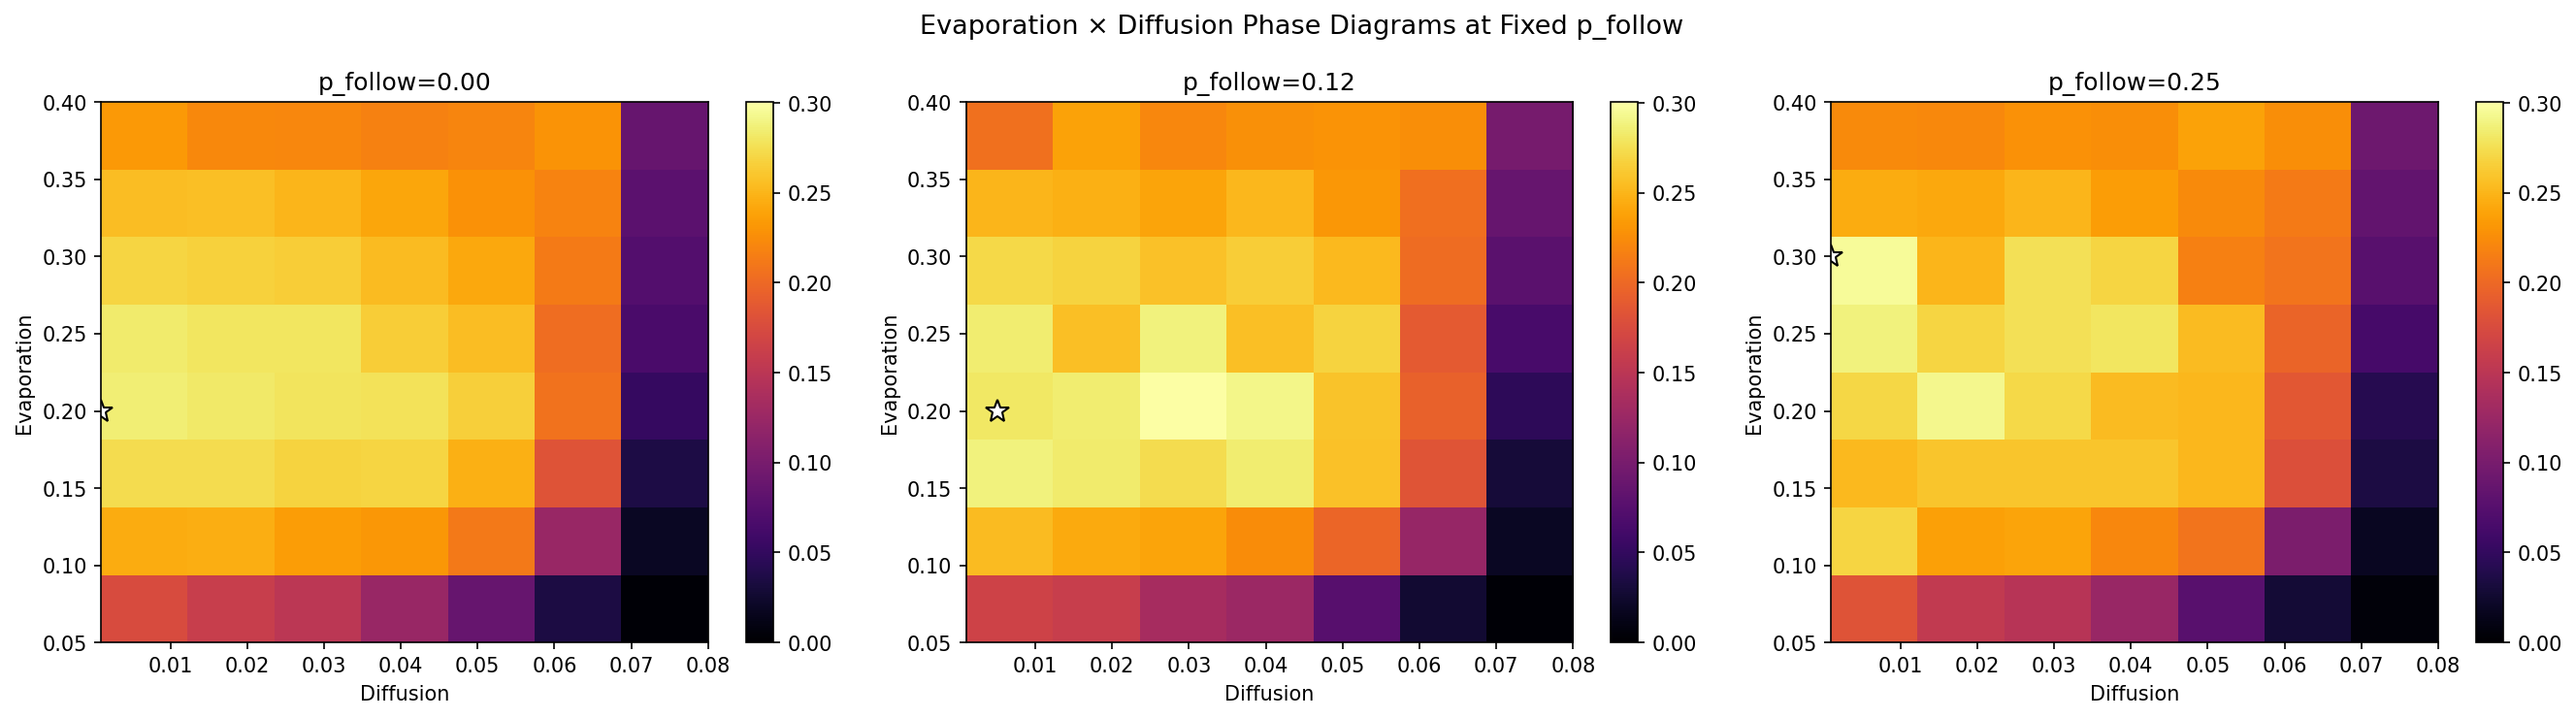
\includegraphics[width=\textwidth]{fig_diffusion_slices.png}
\caption{Evaporation vs diffusion at three fixed $p_f$ values.
  A diagonal band of good composites runs from (low $\lambda$, low $\sigma$) to (high $\lambda$, high $\sigma$): faster-spreading pheromone must evaporate faster to avoid becoming fog.}
\label{fig:diffusion_slices}
\end{figure}

The evaporation--diffusion interaction (Figure~\ref{fig:diffusion_slices}) shows a diagonal band: the two parameters are coupled through the physics of the pheromone field but are not redundant.
Diffusion is genuinely a third independent axis controlling spatial scale, while evaporation controls temporal scale and $p_f$ controls coupling strength.

\subsection{Momentum $\mu = 0.6$}

At $\mu = 0.6$ (forward weighting $1.6\times$ vs sideways), the peak moves to $p_f = 0.042$, $\lambda = 0.16$, $C = 0.301$---even closer to the $p_f = 0$ edge.

\begin{figure}[H]
\centering
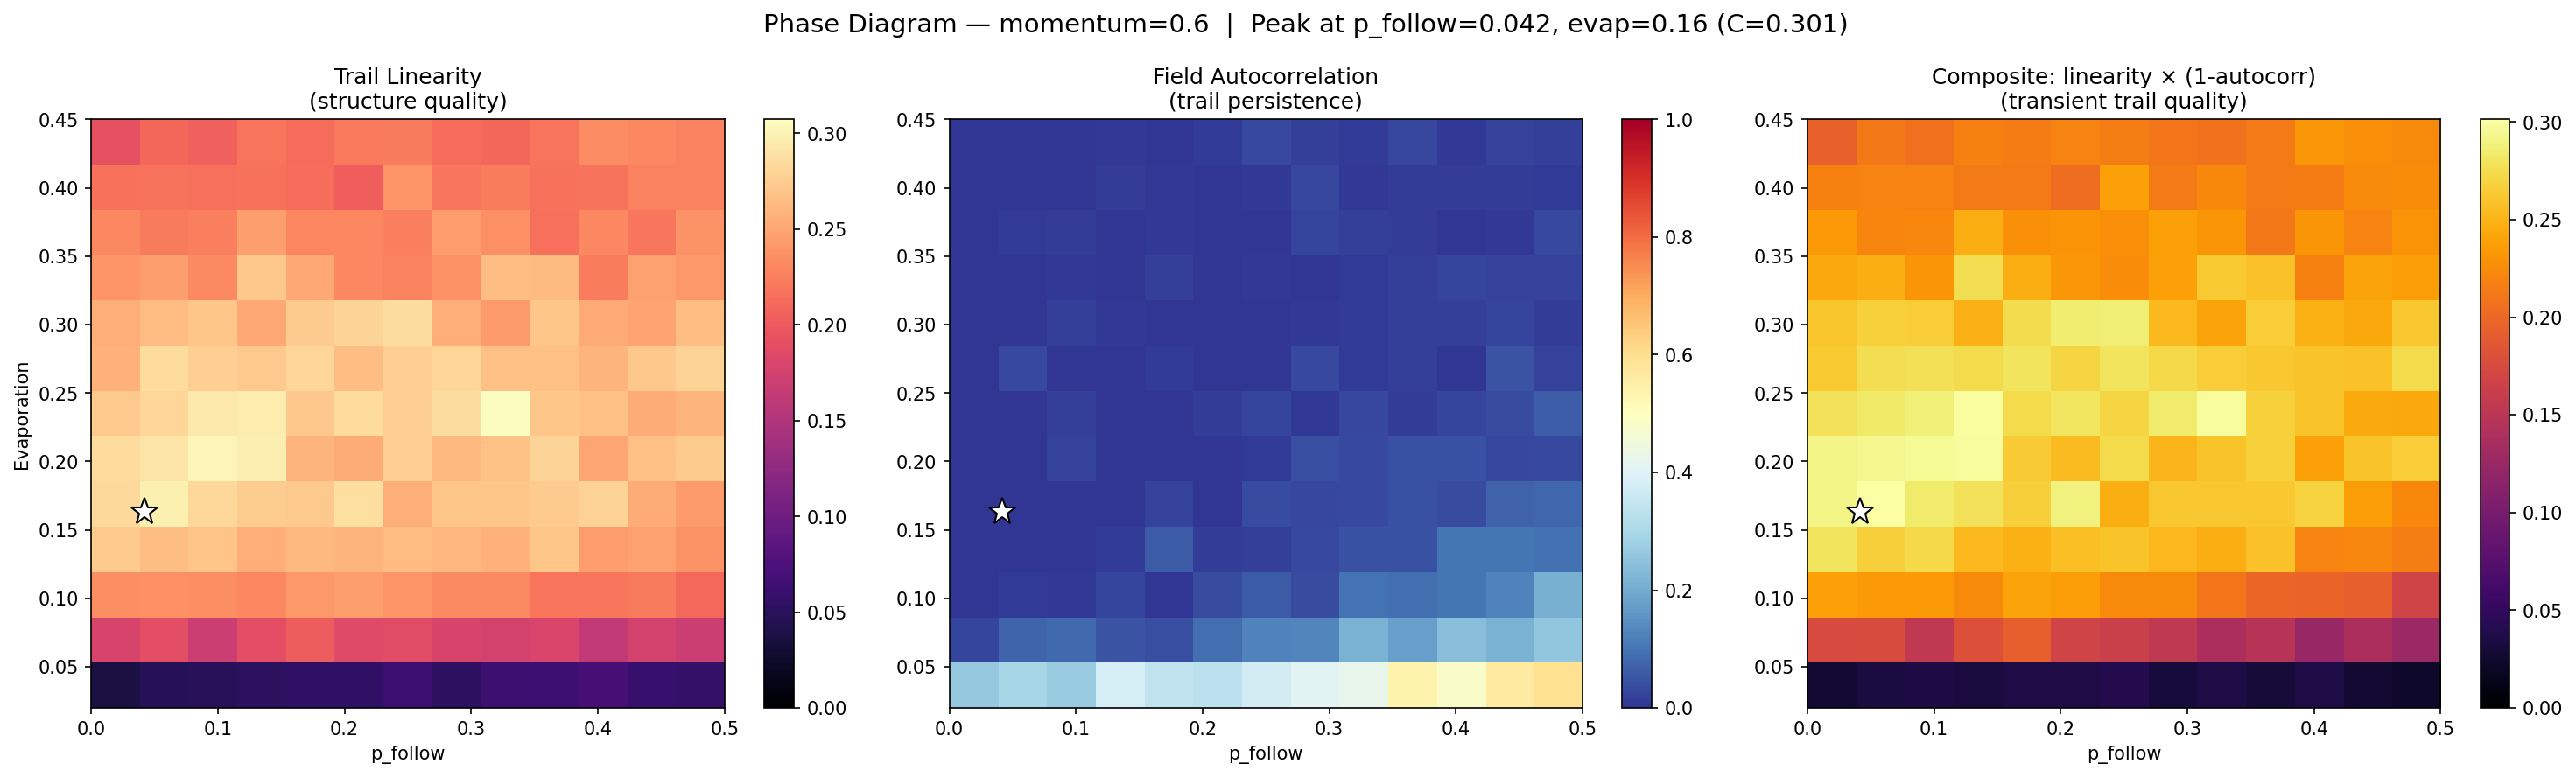
\includegraphics[width=\textwidth]{fig_triptych_mom06.png}
\caption{Phase diagram at $\mu = 0.6$.
  The peak at $p_f = 0.042$ confirms the trend: any momentum above $\sim 0.3$ creates enough spatial structure from random deposition to saturate the linearity metric.}
\label{fig:mom06}
\end{figure}

This confirms the pattern: increasing momentum pushes the composite peak toward $p_f = 0$, because the random-walk branch produces progressively more trail-like structure on its own.

% ================================================================
\section{The Susceptibility Model: State-Dependent Following}
\label{sec:susceptibility}
% ================================================================

\subsection{Motivation}

The simple model's $p_f$ fails because each ant's decision is independent of the field's current state.
Can we achieve sharp transitions through state-dependent coupling instead?

Real ants secrete pheromone continuously as they walk---a chemical byproduct, not a deliberate signal---but only \emph{follow} trails when pheromone concentration exceeds a detection threshold.
This creates feedback: whether an ant follows depends on the pheromone field, which itself depends on whether ants are following.

\subsection{Formulation}

All ants deposit pheromone unconditionally every step (biological secretion).
Movement is state-dependent:

\begin{equation}
  \text{Each step:} \quad
  \begin{cases}
    \text{if } \max_{j \in \mathcal{N}} \phi_j > s: & \text{follow pheromone with momentum} \\
    \text{otherwise:} & \text{walk with momentum only}
  \end{cases}
  \label{eq:susceptibility}
\end{equation}

In both branches, the ant maintains directional persistence (momentum $\mu$).
When following, neighbour weights are $w_j = (\phi_j + 0.01) \times (1 + \mu \cos\theta_j)$: a linear pheromone attraction modulated by the heading direction.
This causes ants to walk \emph{along} trails rather than converging on pheromone peaks, producing linear highways.
When not following, weights are purely momentum-based: $w_j = \max(0.01, 1 + \mu \cos\theta_j)$, producing a gentle meander.

The parameter $s$ is the \emph{susceptibility threshold}---the pheromone concentration an ant must detect in its Moore neighbourhood to begin following.
The key parameters are:

\begin{table}[H]
\centering
\caption{Susceptibility model parameters.}
\label{tab:suscept}
\begin{tabular}{@{}lll@{}}
\toprule
Parameter & Symbol & Role \\
\midrule
Susceptibility threshold & $s$ & Pheromone level needed to trigger following \\
Evaporation & $\lambda$ & Pheromone decay rate \\
Diffusion & $\sigma$ & Pheromone spreading rate \\
\bottomrule
\end{tabular}
\end{table}

Unlike $p_f$, the susceptibility threshold $s$ does not directly set the fraction of ants that follow.
Instead, the follow fraction is an \emph{emergent} quantity determined by the interplay between deposition, evaporation, and the threshold.

\subsection{The positive feedback mechanism}

The susceptibility model creates \textbf{bistable dynamics} through positive feedback: pheromone exceeds threshold $\to$ ants follow $\to$ more deposition on trail $\to$ pheromone stays above threshold (\textbf{lock-in}); conversely, pheromone below threshold $\to$ no following $\to$ evaporation erodes it $\to$ pheromone stays below (\textbf{no trail}).
This creates a sharp phase boundary between ``all recruited'' and ``none recruited,'' determined by the balance of deposition rate, evaporation, and susceptibility threshold.
Unlike the noise model's external destruction, criticality here arises from the system's own feedback dynamics.

\subsection{Sweep results}

We swept 17 susceptibility values ($s \in [0.05, 20]$), 16 evaporation values ($\lambda \in [0.05, 0.50]$), and 4 diffusion rates ($\sigma \in \{0.002, 0.005, 0.010, 0.020\}$), totalling 1{,}088 simulations on an $80 \times 80$ grid with $\mu = 2.0$, $\delta = 5.0$, and 800 steps.
The composite uses block variance: $C = B \times (1 - A)$.

\begin{figure}[H]
\centering
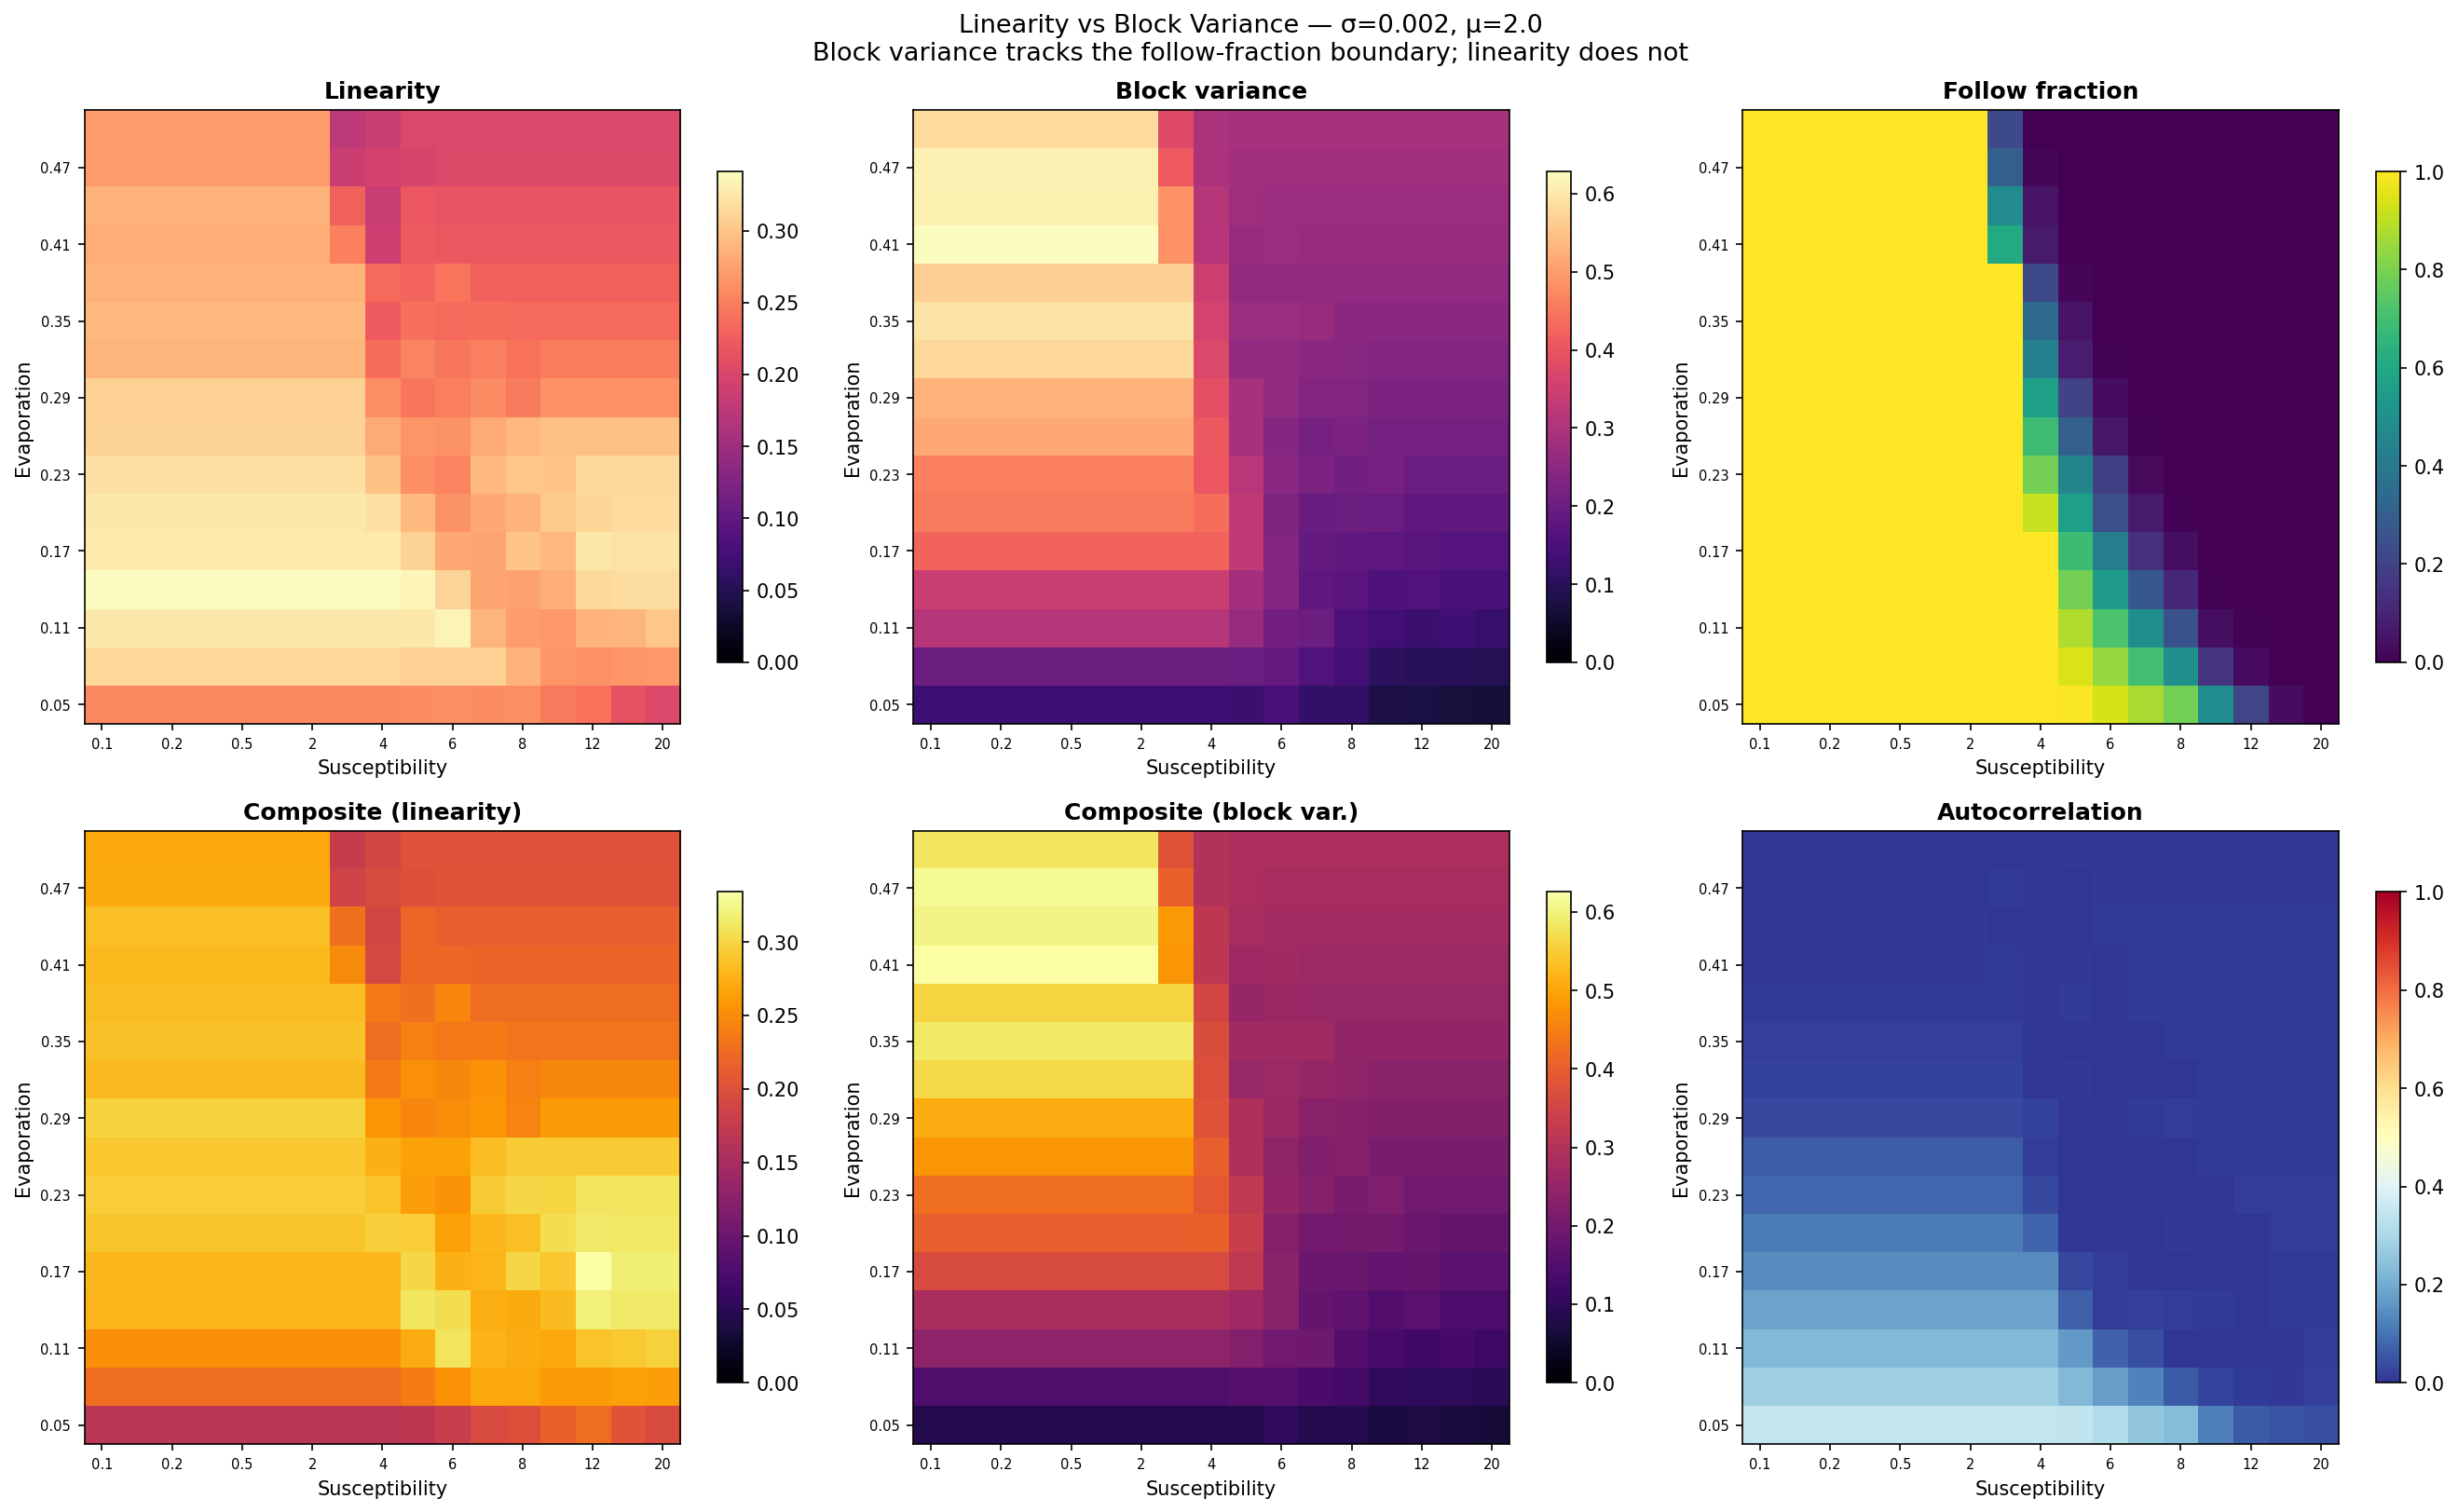
\includegraphics[width=\textwidth]{fig_suscept_v2_comparison.png}
\caption{Linearity vs block variance as structure metrics.
  Top row: linearity, block variance, and follow fraction.
  Bottom row: composites formed with each metric, and autocorrelation.
  Linearity is nearly flat across regimes ($\sim$10\% variation).
  Block variance tracks the follow-fraction boundary, dropping by $\sim$50\% when following ceases.}
\label{fig:suscept_comparison}
\end{figure}

Figure~\ref{fig:suscept_comparison} compares the two metrics: linearity is flat across regimes; block variance tracks the follow-fraction boundary.

\begin{figure}[H]
\centering
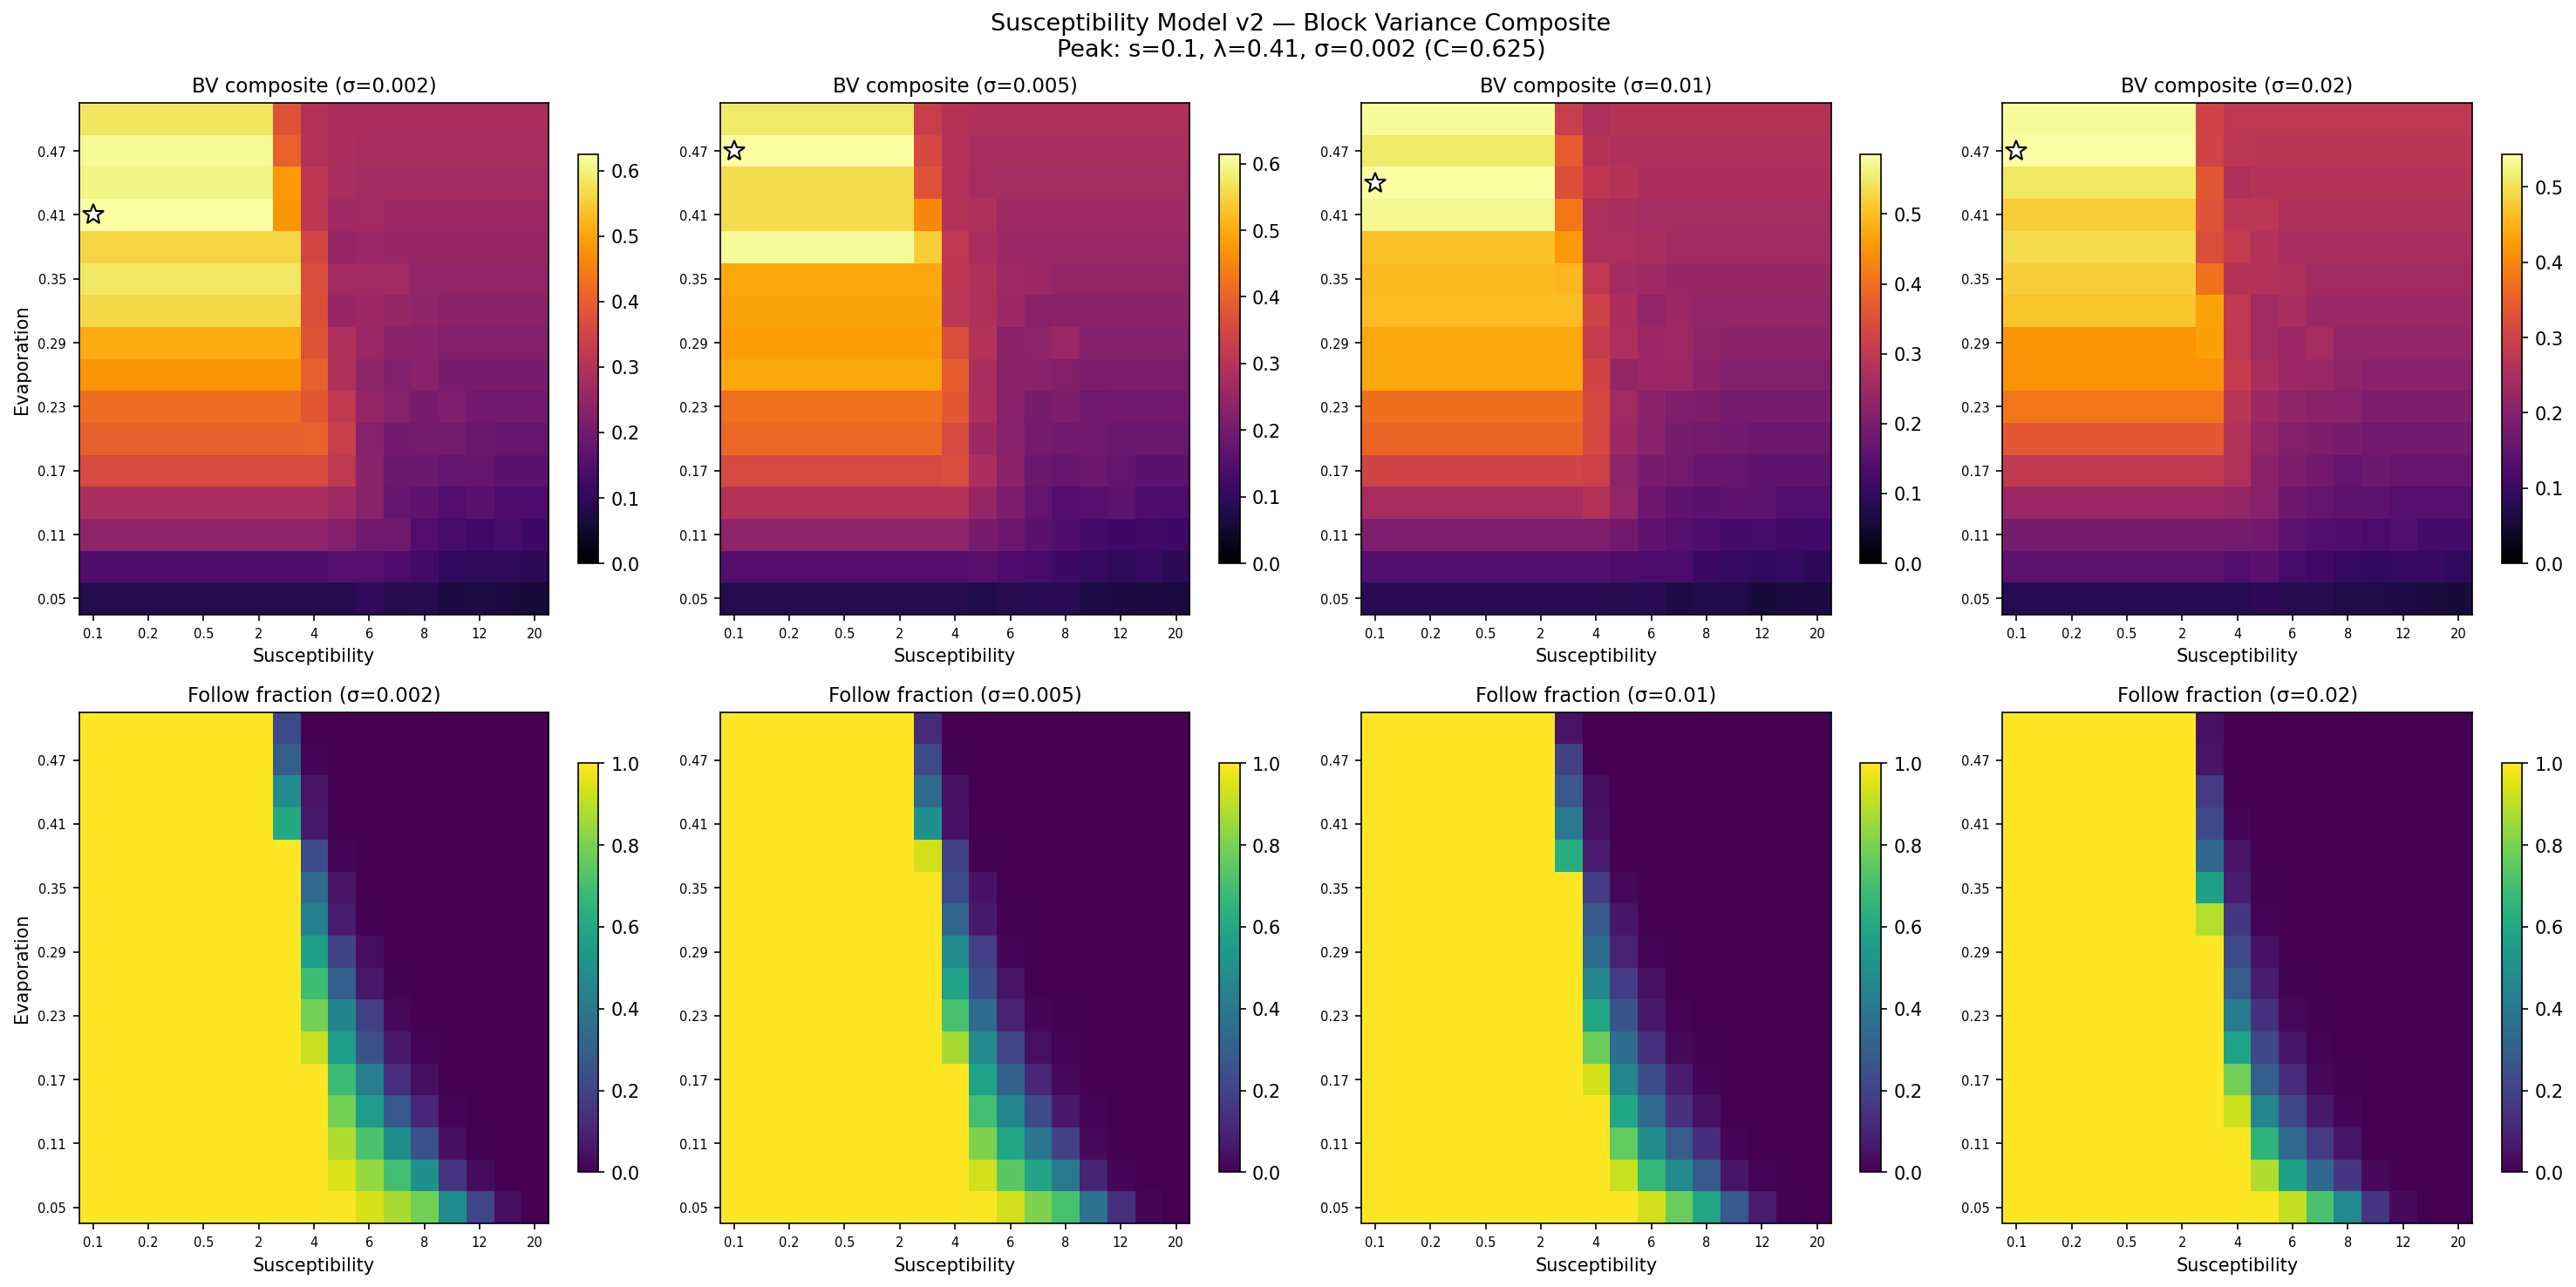
\includegraphics[width=\textwidth]{fig_suscept_v2_grid.png}
\caption{Block variance composite and follow fraction across four diffusion rates.
  Top row: composite $C = B \times (1-A)$. Bottom row: follow fraction.
  The composite peak (star) sits in the high-evaporation, low-susceptibility regime where all ants follow but evaporation constantly reshapes the trail network---erosion-driven transience.
  Higher diffusion shifts the follow-fraction boundary rightward (pheromone spreads further, lowering the effective detection threshold).}
\label{fig:suscept_v2_grid}
\end{figure}

The phase diagram (Figure~\ref{fig:suscept_v2_grid}) reveals three regimes:

\begin{itemize}
  \item \textbf{Frozen} (low $s$, low $\lambda$): Nearly 100\% of ants follow.
    Persistent highway networks with high autocorrelation and high block variance.
  \item \textbf{Transient} (moderate $s$, moderate $\lambda$): Partial recruitment.
    The follow fraction transitions sharply from high to zero.
    Trails form, attract followers, strengthen, get eroded, collapse, and reform elsewhere.
  \item \textbf{No following} (high $s$ or high $\lambda$): Follow fraction drops to zero.
    Only unconditional deposition remains; block variance is low.
\end{itemize}

The follow-fraction boundary is a sharp diagonal---a genuine phase transition produced by positive feedback, not the smooth crossover seen in the $p_f$ model.
The transition curves (Figure~\ref{fig:suscept_transitions}) are nearly vertical sigmoids, steepening at low evaporation where positive feedback is strongest.

\begin{figure}[H]
\centering
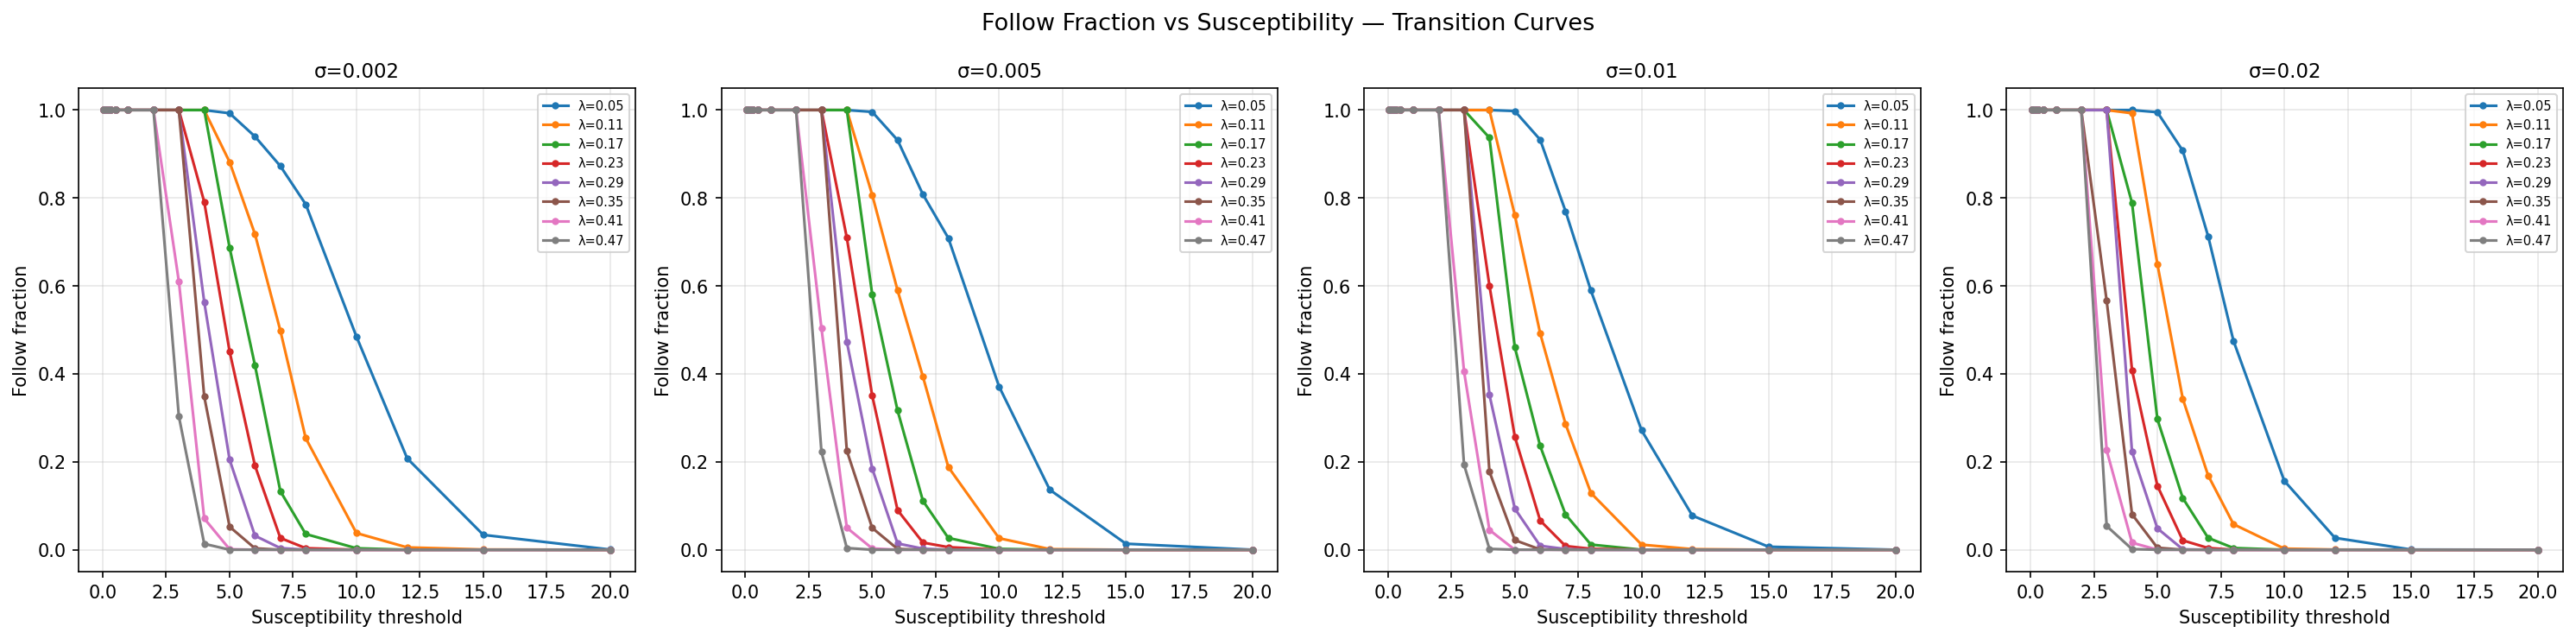
\includegraphics[width=\textwidth]{fig_suscept_v2_transitions.png}
\caption{Follow fraction vs susceptibility threshold at each diffusion rate, coloured by evaporation.
  The transition steepens at low evaporation (stronger positive feedback).}
\label{fig:suscept_transitions}
\end{figure}

\begin{figure}[H]
\centering
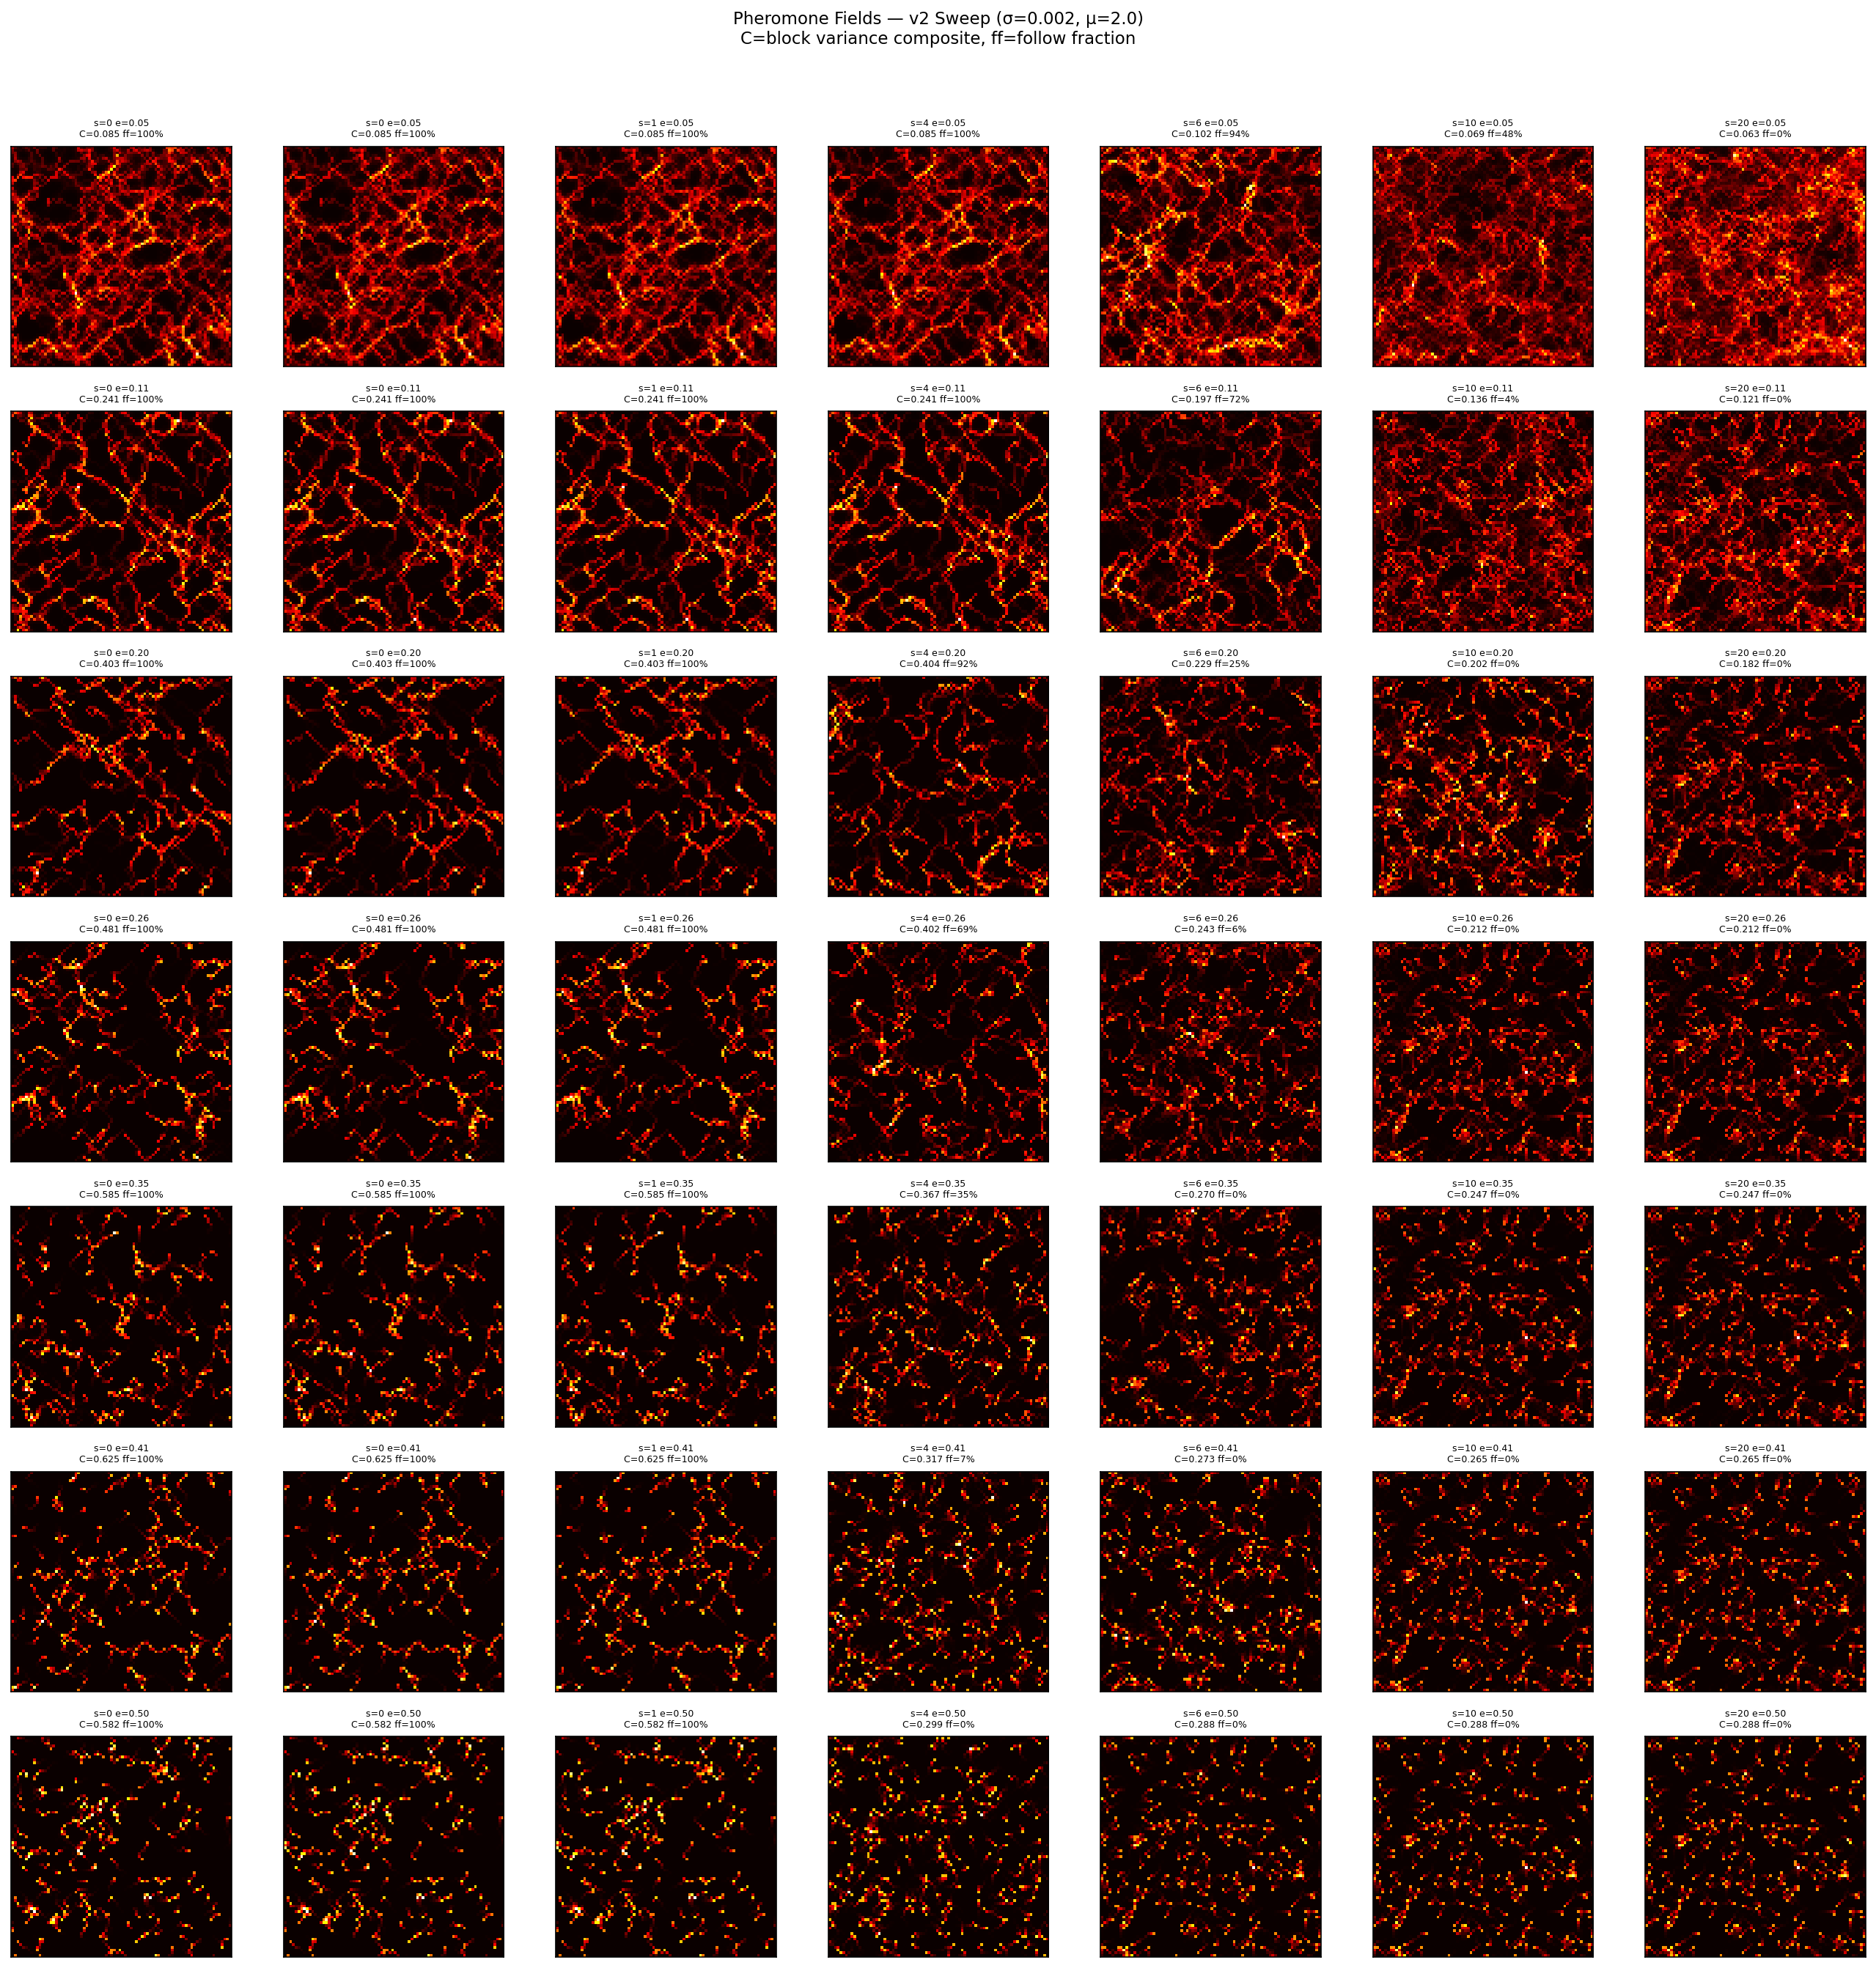
\includegraphics[width=\textwidth]{fig_suscept_v2_snapshots.png}
\caption{Pheromone fields across the susceptibility--evaporation plane.
  Low susceptibility (left): bright highway networks from near-total recruitment.
  High susceptibility (right): uniform dim glow from unconditional deposition alone.
  The transition from trails to disorder is visually abrupt, matching the sharp follow-fraction boundary.}
\label{fig:suscept_snapshots}
\end{figure}

% ================================================================
\section{Study 4: Decoupling Recruitment and Persistence}
\label{sec:decoupling}
% ================================================================

The composite peaked not at the recruitment boundary but in the erosion-driven transience regime ($s = 0.1$, $\lambda = 0.41$, $f = 1.0$, $C = 0.625$).
This section investigates why.

\subsection{Why the standard composite misses the recruitment boundary}

The composite $C = B \times (1 - A)$ rewards configurations that are simultaneously \emph{structured} (high $B$) and \emph{transient} (low $A$).
At the recruitment boundary, $B$ is declining (fewer followers means weaker trails) even though $A$ is also low.
In the all-following regime at high evaporation, $B$ remains maximal while $A$ drops---yielding a higher product.
The composite therefore peaks not at the recruitment boundary but in the erosion-driven regime.

\subsection{A recruitment-sensitive composite}

To target the recruitment phase boundary specifically, we introduce a recruitment weighting factor:
\begin{equation}
  C_R = B \times (1 - A) \times 4 f (1 - f)
  \label{eq:recruit_composite}
\end{equation}
where $f$ is the follow fraction.
The factor $4 f(1-f)$ is maximised at $f = 0.5$ (half the ants following) and vanishes at $f = 0$ and $f = 1$, forcing the composite to peak at the recruitment transition rather than deep in the ordered or disordered regime.

\begin{figure}[H]
\centering
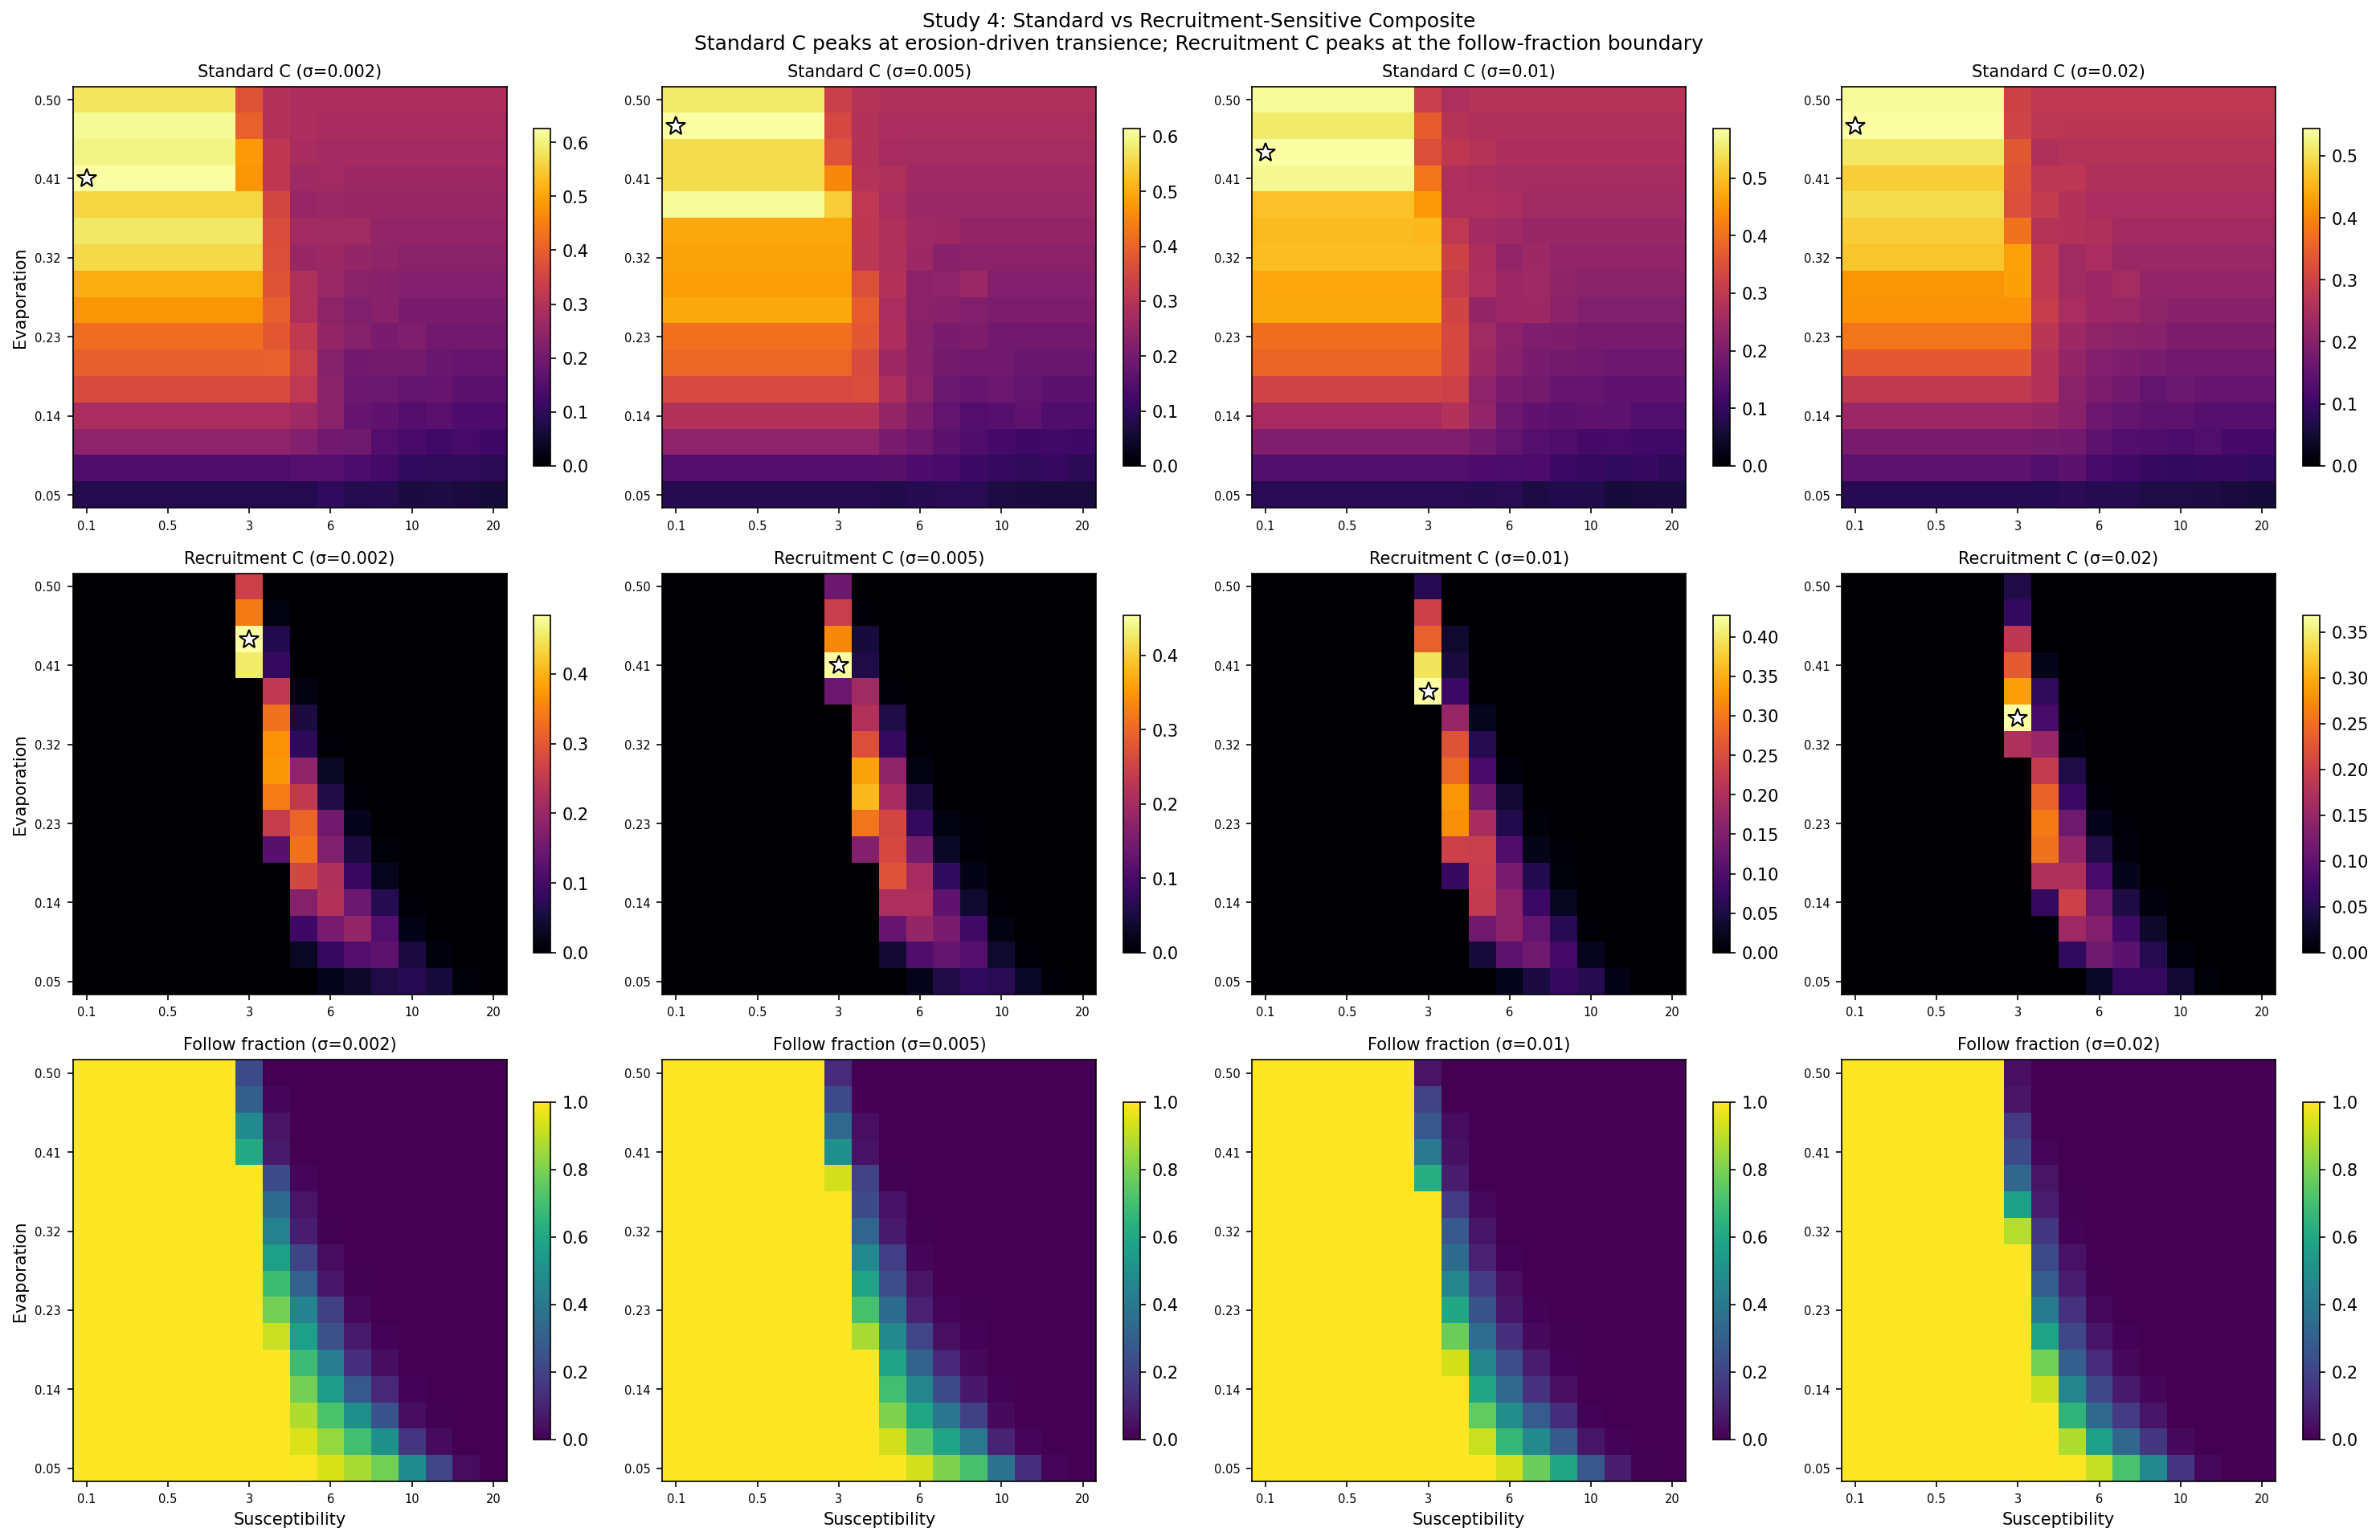
\includegraphics[width=\textwidth]{fig_study4_composites.png}
\caption{Standard vs recruitment-sensitive composite across four diffusion rates.
  Top row: standard $C = B \times (1-A)$, peaking in the all-following regime (top-left, star).
  Middle row: recruitment composite $C_R = B \times (1-A) \times 4f(1-f)$, peaking at the follow-fraction boundary (star on diagonal).
  Bottom row: follow fraction for reference.
  The two composites locate different phenomena in the same parameter space.}
\label{fig:study4_composites}
\end{figure}

$C_R$ peaks at $s = 3.0$, $\lambda = 0.44$, $\sigma = 0.002$ with $C_R = 0.484$ and $f = 0.48$---precisely at the recruitment boundary (Figure~\ref{fig:study4_composites}).

\begin{figure}[H]
\centering
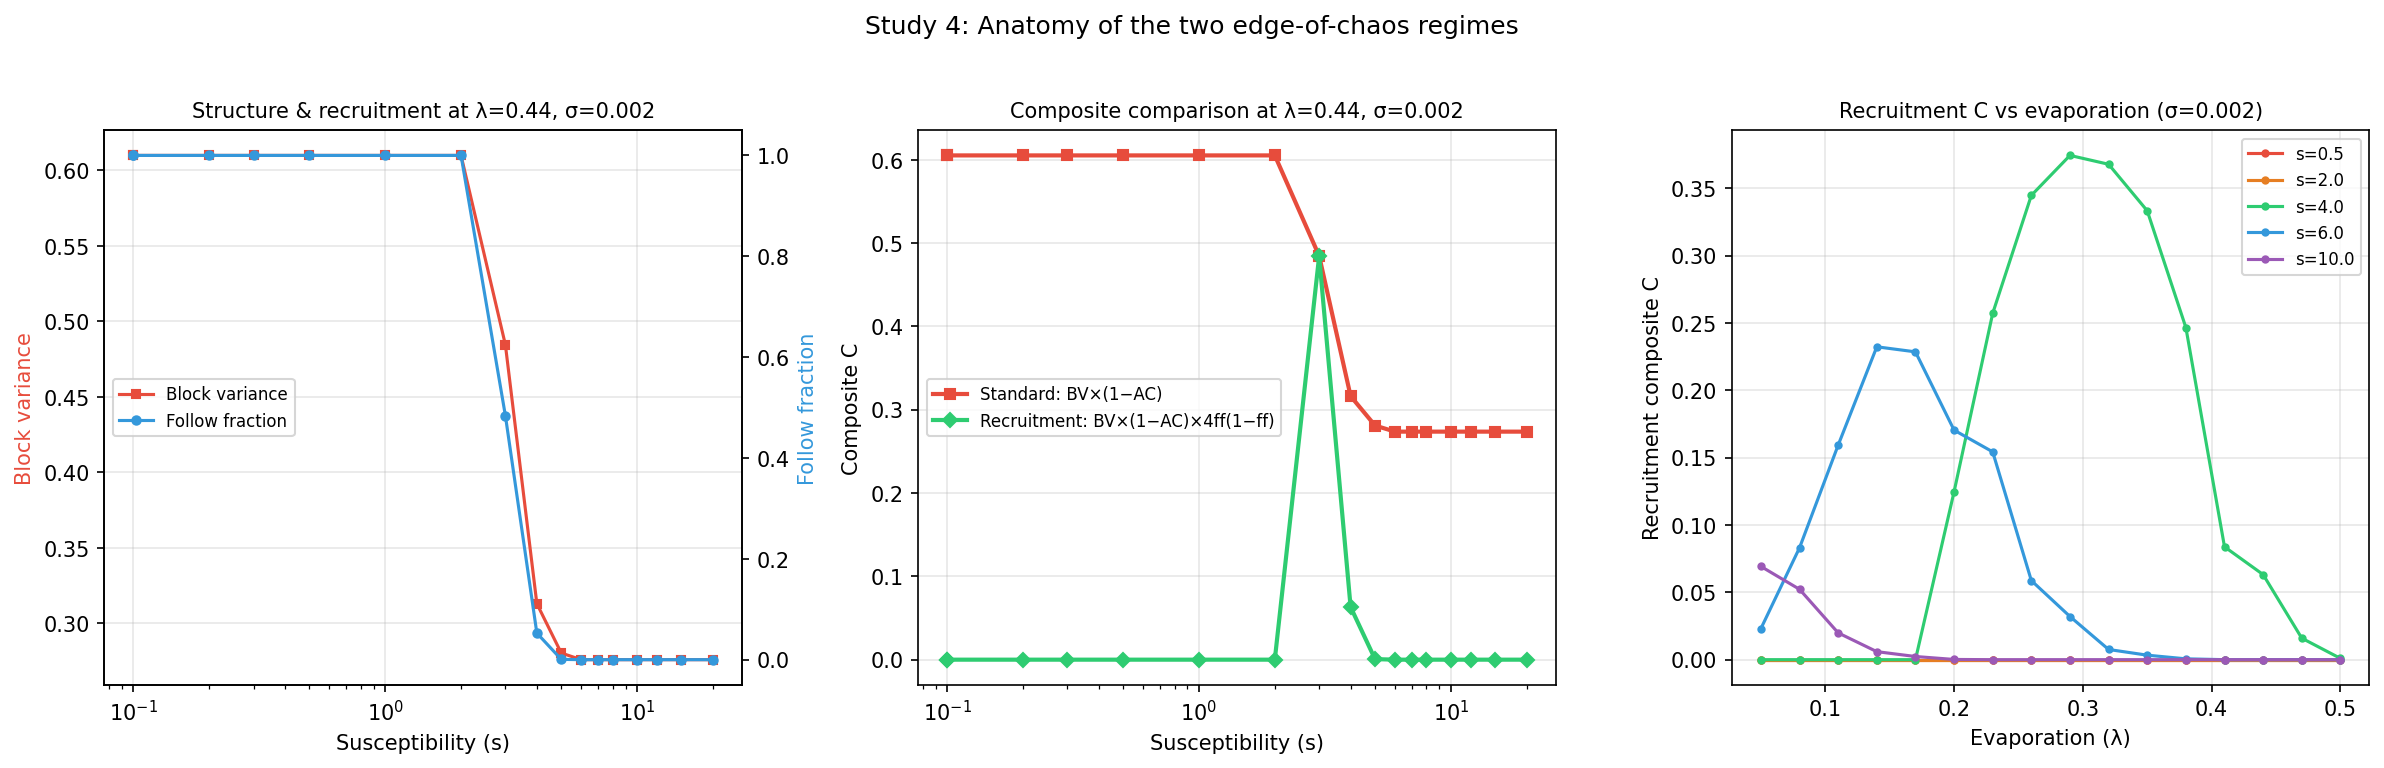
\includegraphics[width=\textwidth]{fig_study4_slices.png}
\caption{One-dimensional slices at the recruitment composite peak ($\lambda = 0.44$, $\sigma = 0.002$).
  Left: block variance and follow fraction vs susceptibility.
  Centre: both composites vs susceptibility---standard $C$ drops monotonically; $C_R$ peaks at $s \approx 3$ where $f \approx 0.5$.
  Right: $C_R$ vs evaporation at several susceptibility values.}
\label{fig:study4_slices}
\end{figure}

\subsection{A sharp phase transition that is not edge of chaos}

Across the recruitment boundary, $C$ drops \emph{monotonically}: at $\lambda = 0.44$, $C = 0.605$ at $s = 2$ (all following), $C = 0.485$ at $s = 3$ ($f = 0.48$), and $C = 0.316$ at $s = 4$ (no following).
$B$ and $A$ decline together---fewer followers means weaker trails \emph{and} less persistence.
The recruitment boundary is a \textbf{sharp phase transition} ($\Delta f > 0.7$ in a single step) but \textbf{not edge of chaos}: a first-order-like collapse between attractors with no intermediate critical regime.

\subsection{Erosion-driven transience: the true edge of chaos}

The composite peaks at $C = 0.625$ in a different region: $s = 0.1$, $\lambda = 0.41$, $f = 1.0$.
All ants follow, but evaporation erodes trails faster than they can freeze---the network is maximally structured yet constantly reshuffling.
This is genuine edge of chaos along the \emph{persistence axis}.

\subsection{Why the original model's ridge was a superposition}

The noise parameter $\varepsilon$ simultaneously reduces recruitment (ants ignore pheromone) \emph{and} persistence (disrupted deposition weakens trails), producing a single ridge.
The susceptibility model separates these into orthogonal axes, revealing a superposition of erosion-driven transience (genuine edge of chaos, $C = 0.625$) and a recruitment phase transition (sharp but not edge of chaos---$C$ drops monotonically, located by $C_R$ at $f \approx 0.5$).

% ================================================================
\section{Study 5: Finding the Edge of Chaos}
\label{sec:negative_feedback}
% ================================================================

Studies 3 and 4 established that the susceptibility model's recruitment boundary is a sharp phase transition but \emph{not} edge of chaos---the composite drops monotonically across it.
The genuine edge of chaos (erosion-driven transience) operates along the persistence axis via an environmental mechanism (evaporation).
Can we achieve edge of chaos through a mechanism intrinsic to the ant?

\subsection{The recipe: decoupling structure from persistence}

Edge of chaos requires $B$ to stay high while $A$ drops---trails must be strong yet transient.
The susceptibility model's recruitment boundary fails because $B$ and $A$ decline together (only positive feedback).
A mechanism that keeps trails strong while making them shift location would decouple $B$ from $A$.
The original model achieves this \emph{externally} (noise) and \emph{environmentally} (evaporation).
Can an \emph{intrinsic} ant-level mechanism do the same?

\subsection{Candidate mechanisms}

We test three intrinsic mechanisms, built on top of the susceptibility model:

\begin{enumerate}
  \item \textbf{Habituation} (sensory adaptation).
    Each ant maintains an internal habituation counter $h$.
    While following a trail, $h$ increments by 1 each step.
    When $h \geq \tau_h$ (the habituation timescale), the ant becomes desensitised: it stops following pheromone \emph{and} stops depositing it (habituated ants contribute nothing to the trail network).
    Recovery is $5\times$ faster than habituation, so the steady-state follow fraction is $\sim$83\%.
    The ant resumes following only after $h$ decays back to zero (hysteresis prevents rapid oscillation).
    Initial habituation counters are randomised to desynchronise the population.
    The control parameter is $\tau_h$: the number of following steps before an ant habituates.
    Fixed susceptibility $s = 2.0$ (all-following regime).

  \item \textbf{Peaked pheromone response} (sensory saturation).
    Rather than removing ants from trails, this mechanism modifies \emph{how} ants perceive pheromone.
    The effective pheromone field used for movement decisions is $\phi_\text{eff} = \phi \cdot e^{-\phi / \phi_\text{sat}}$, which peaks at $\phi = \phi_\text{sat}$ and decreases above it.
    Ants are most attracted to moderately concentrated trails; extremely strong trails lose their attractiveness advantage.
    This keeps $f = 1$ (all ants always follow) but redistributes ants across competing trail segments.
    The control parameter is $\phi_\text{sat}$: the pheromone concentration at peak attractiveness.
    Fixed susceptibility $s = 2.0$.

  \item \textbf{Hill function} (soft sigmoid threshold).
    This replaces the hard susceptibility threshold with a biologically realistic chemoreceptor model:
    \begin{equation}
      P(\text{follow}) = \frac{\phi^n}{\phi^n + s^n}
      \label{eq:hill}
    \end{equation}
    where $\phi$ is the maximum pheromone in the Moore neighbourhood, $s$ is the half-maximum concentration, and $n$ is the Hill coefficient (steepness).
    At $n = 1$, the response is hyperbolic (near-linear at low $\phi$); as $n \to \infty$, it recovers the hard threshold.
    This creates \emph{state-dependent noise}: strong trails are followed reliably, weak trails unreliably.
    Unlike the external noise parameter, this noise is intrinsic to the ant's sensory process and correlated with the pheromone field.
    Swept: $s \in [0.5, 20]$ and $\lambda \in [0.05, 0.50]$ at $n \in \{1, 2, 4\}$, compared against the hard threshold.
\end{enumerate}

Habituation and peaked response are swept against evaporation $\lambda \in [0.05, 0.50]$ at fixed $s = 2.0$ and $\sigma = 0.005$ (10 values each axis, 100 simulations per mechanism).
The Hill function sweep uses 9 susceptibility values $\times$ 10 evaporation values $\times$ 3 steepness values = 270 simulations, plus 90 hard-threshold comparisons.

\subsection{Results: no mechanism produces intrinsic edge of chaos}

\textbf{Habituation} ($\tau_h \times \lambda$, 100 simulations): The composite peaks at $\tau_h = 400$, $\lambda = 0.50$ ($C = 0.678$, $f = 0.85$)---the boundary of the swept range.
Increasing $\tau_h$ monotonically increases $C$ by keeping more ants following for longer.
No intermediate $\tau_h$ produces a peak.

\textbf{Peaked response} ($\phi_\text{sat} \times \lambda$, 100 simulations): The composite peaks at $\phi_\text{sat} = 0$ (no modification), $\lambda = 0.45$ ($C = 0.639$, $f = 1.00$).
Introducing a peaked response at any saturation level reduces the composite.

\begin{figure}[H]
\centering
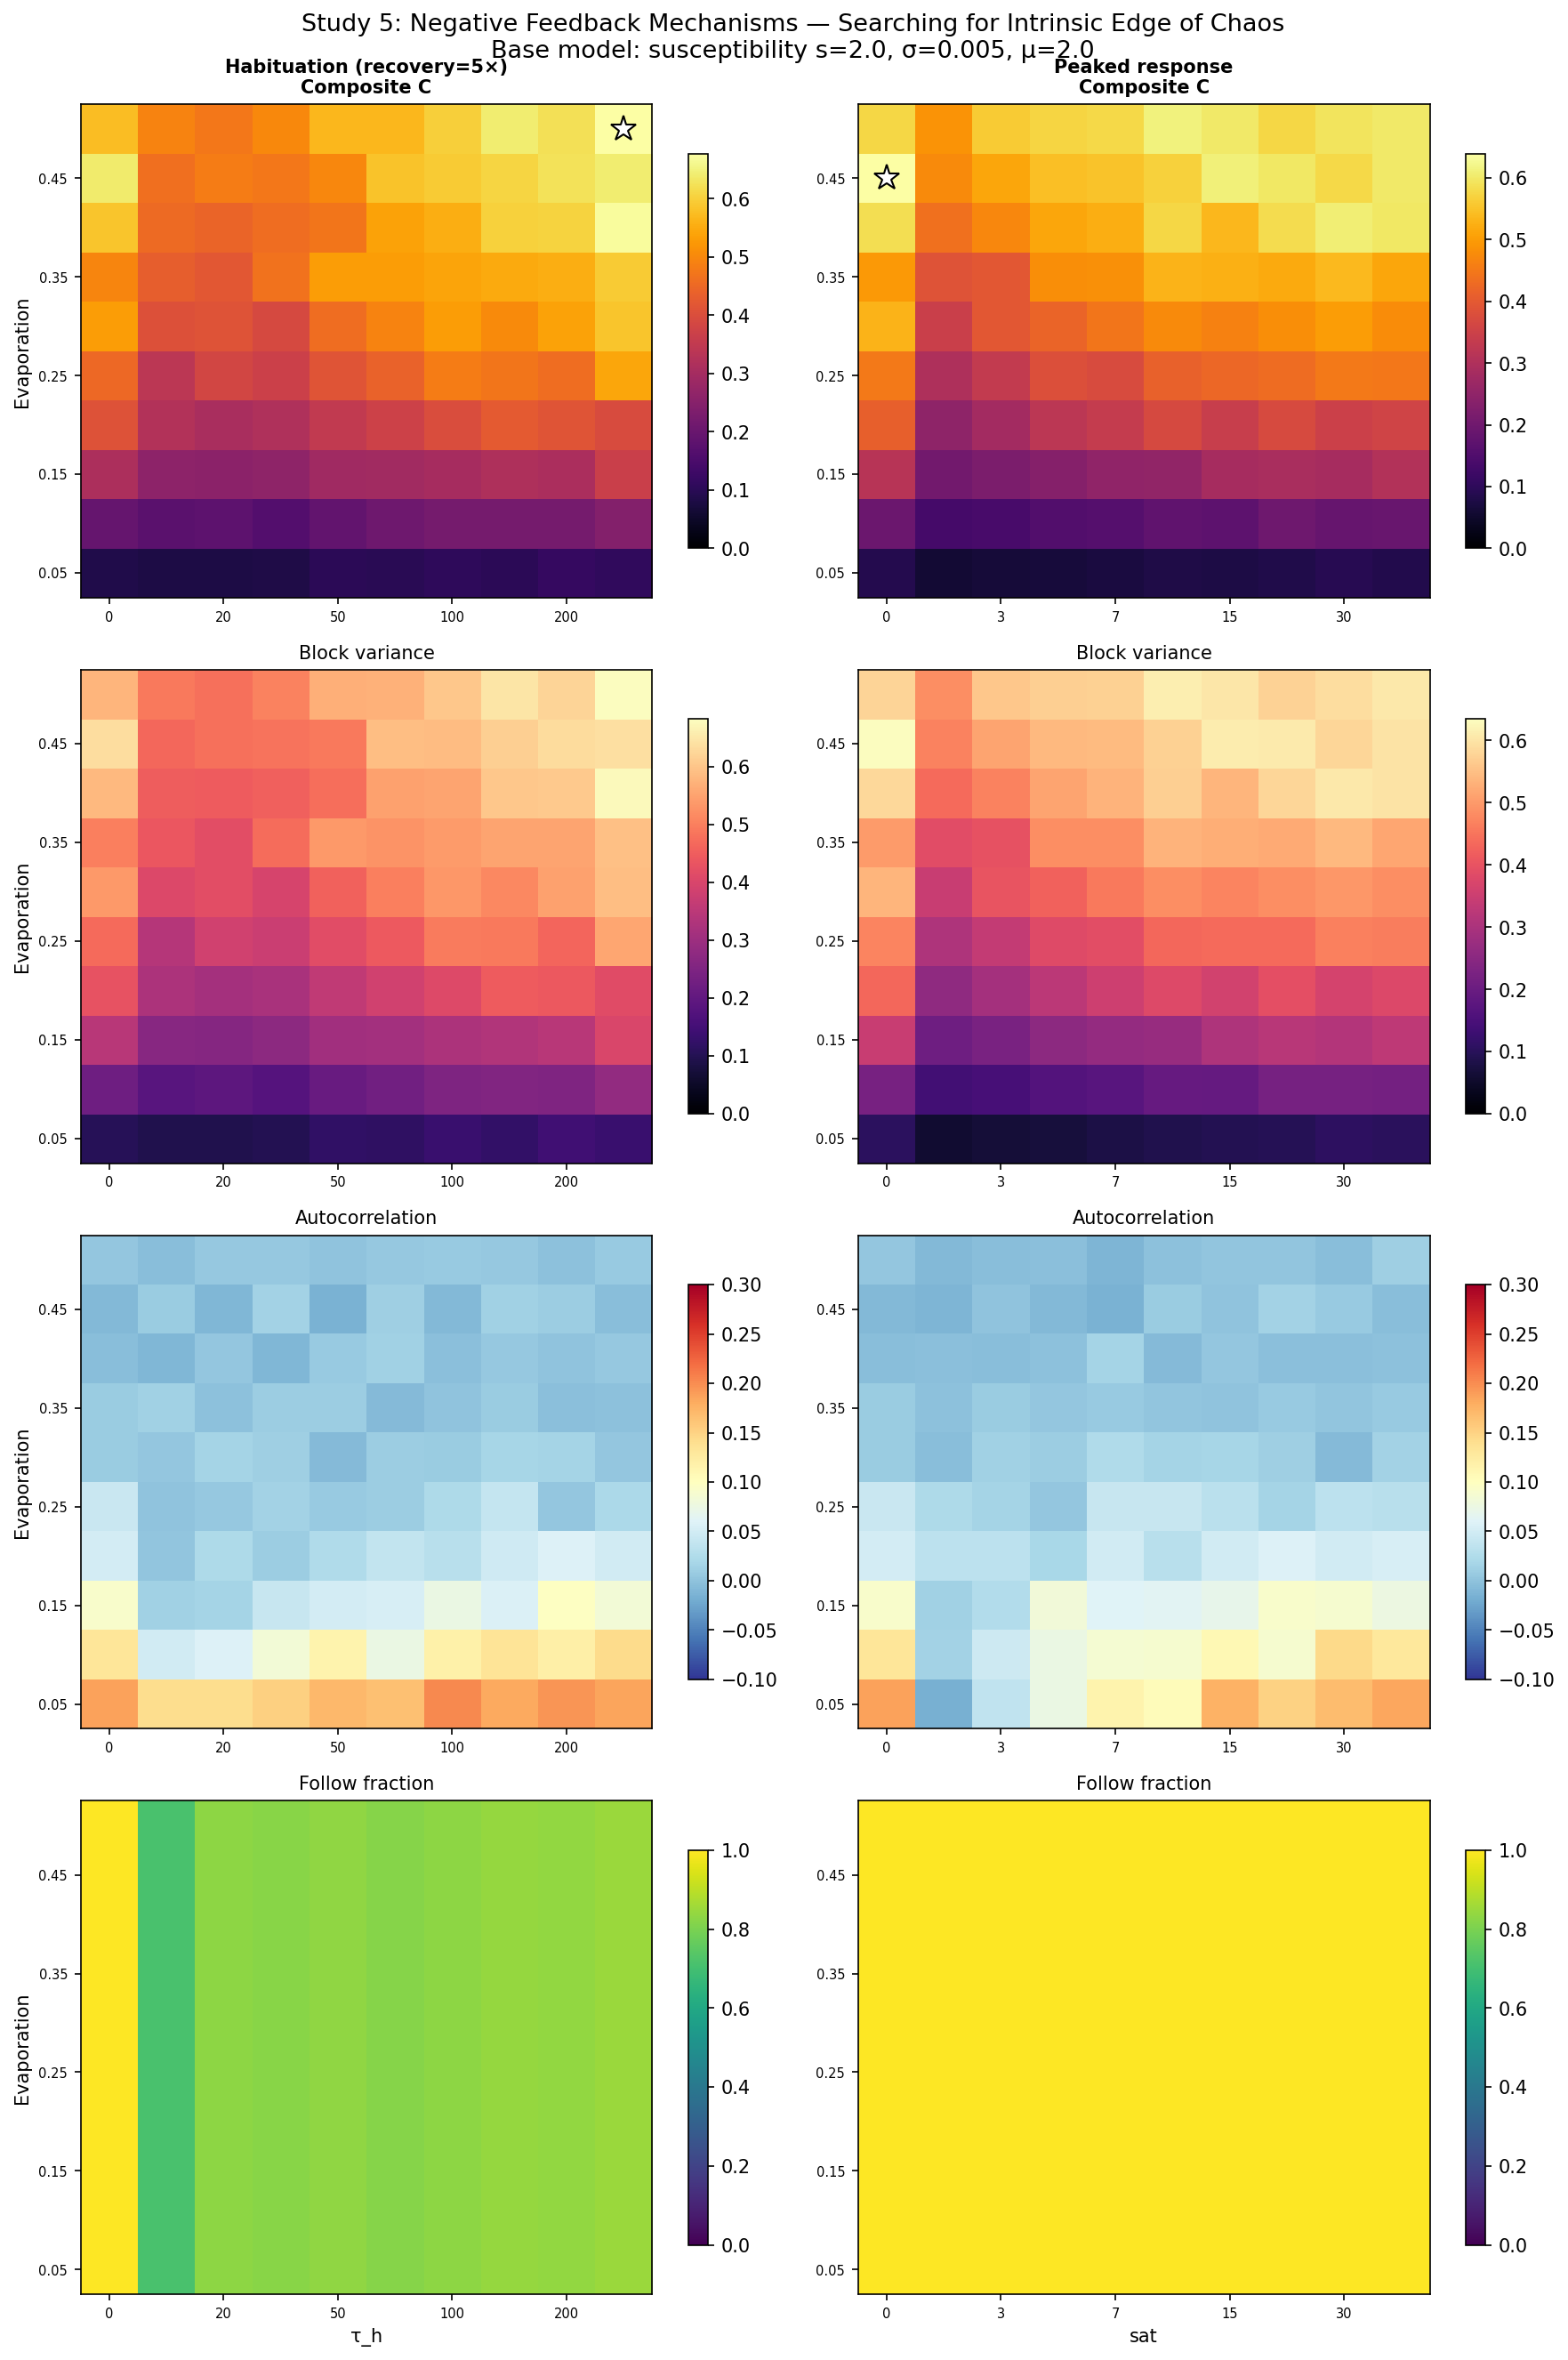
\includegraphics[width=\textwidth]{fig_study5_heatmaps.png}
\caption{Composite order parameter, block variance, autocorrelation, and follow fraction for habituation and peaked response.
  Stars mark composite peaks, both at the boundary of the swept range.
  Neither produces the inverted-U signature of intrinsic edge of chaos.}
\label{fig:study5_heatmaps}
\end{figure}

\textbf{Hill function} ($s \times \lambda$ at $n \in \{1, 2, 4\}$, 360 simulations): The Hill function creates a smooth follow-fraction gradient---at $n = 1$, $s = 2$, $\lambda = 0.50$, the follow fraction is $f = 0.65$ rather than collapsing sharply to zero---but the composite still peaks at the lowest susceptibility ($s = 0.5$) where nearly all ants follow.
At no steepness value does the composite peak at an intermediate susceptibility.

\begin{table}[H]
\centering
\caption{Hill function sweep results. All composite peaks occur at $s = 0.5$ (boundary, not interior).}
\label{tab:hill}
\small
\begin{tabular}{@{}lccccl@{}}
\toprule
Threshold & Peak $s$ & Peak $\lambda$ & $C$ & $f$ & Interior in $s$? \\
\midrule
Hard & 0.5 & 0.45 & 0.639 & 1.00 & No (boundary) \\
Hill $n{=}1$ & 0.5 & 0.35 & 0.496 & 0.89 & No (boundary) \\
Hill $n{=}2$ & 0.5 & 0.45 & 0.597 & 0.98 & No (boundary) \\
Hill $n{=}4$ & 0.5 & 0.50 & 0.581 & 1.00 & No (boundary) \\
\bottomrule
\end{tabular}
\end{table}

\begin{figure}[H]
\centering
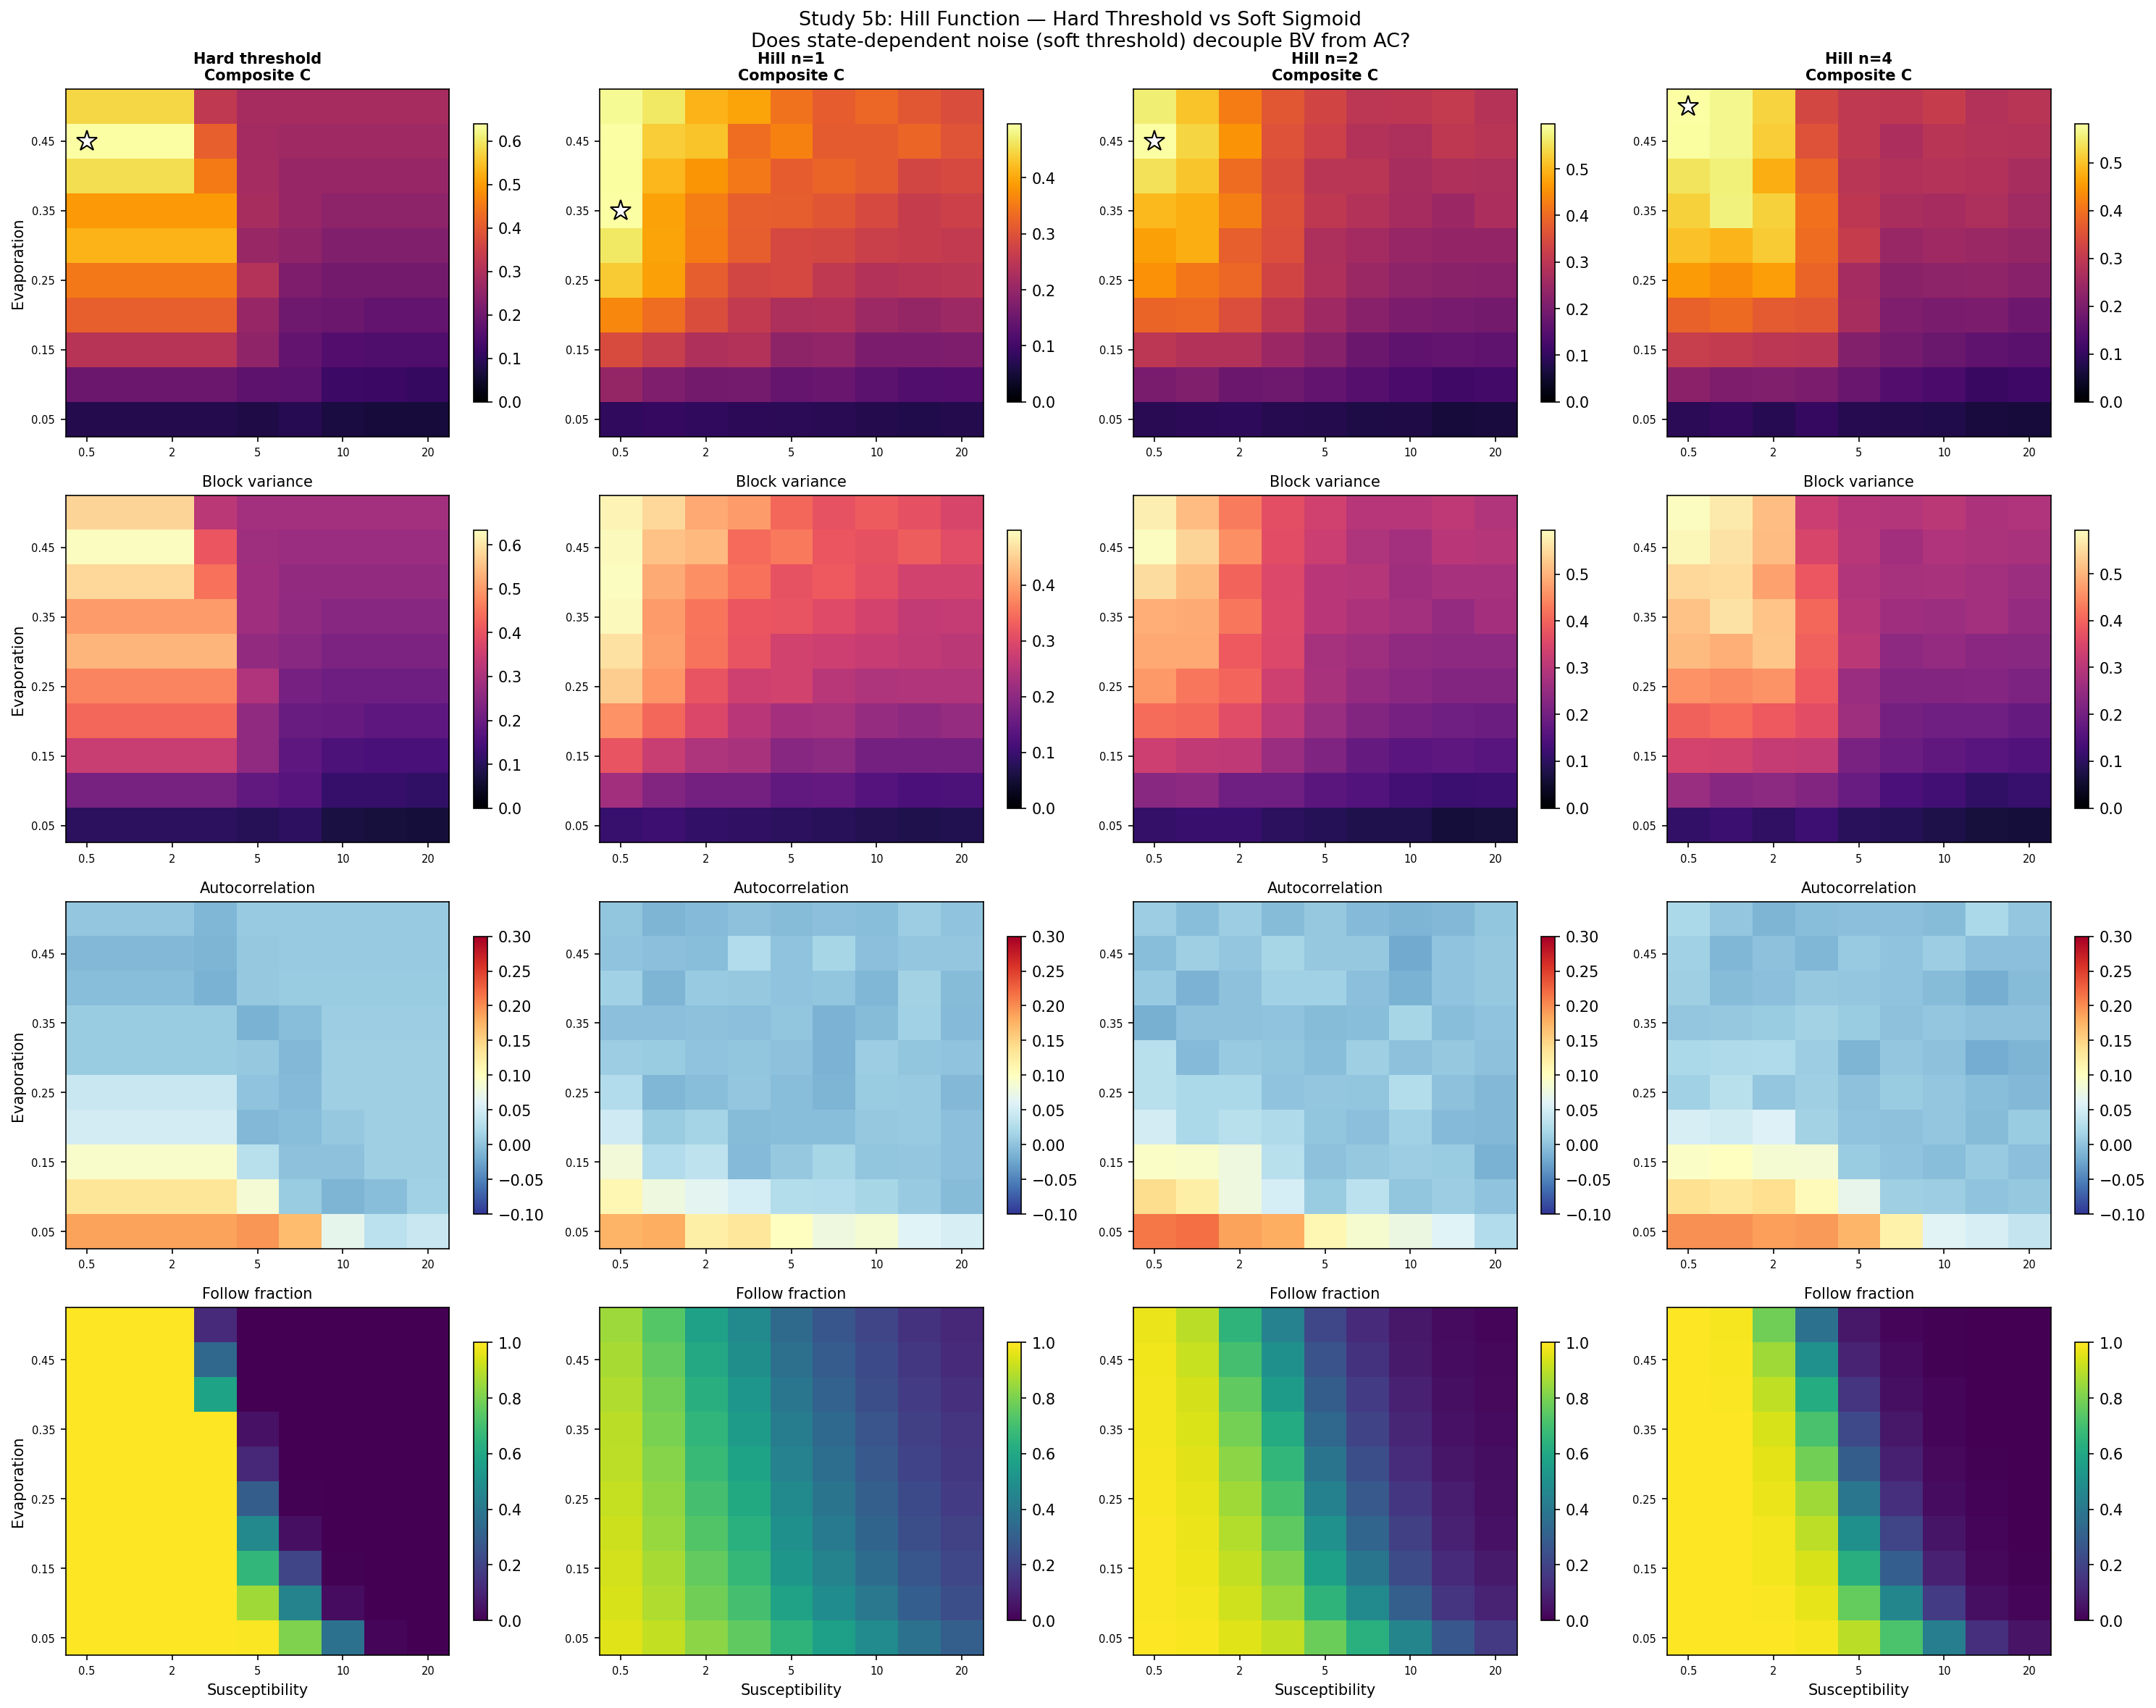
\includegraphics[width=\textwidth]{fig_study5b_heatmaps.png}
\caption{Hard threshold vs Hill function at three steepness values.
  Top row: composite $C$; lower rows: block variance, autocorrelation, follow fraction.
  The Hill function smooths the follow-fraction transition (especially at $n = 1$) but the composite always peaks at the lowest susceptibility (highest following), not at the recruitment boundary.}
\label{fig:study5b_heatmaps}
\end{figure}

\begin{figure}[H]
\centering
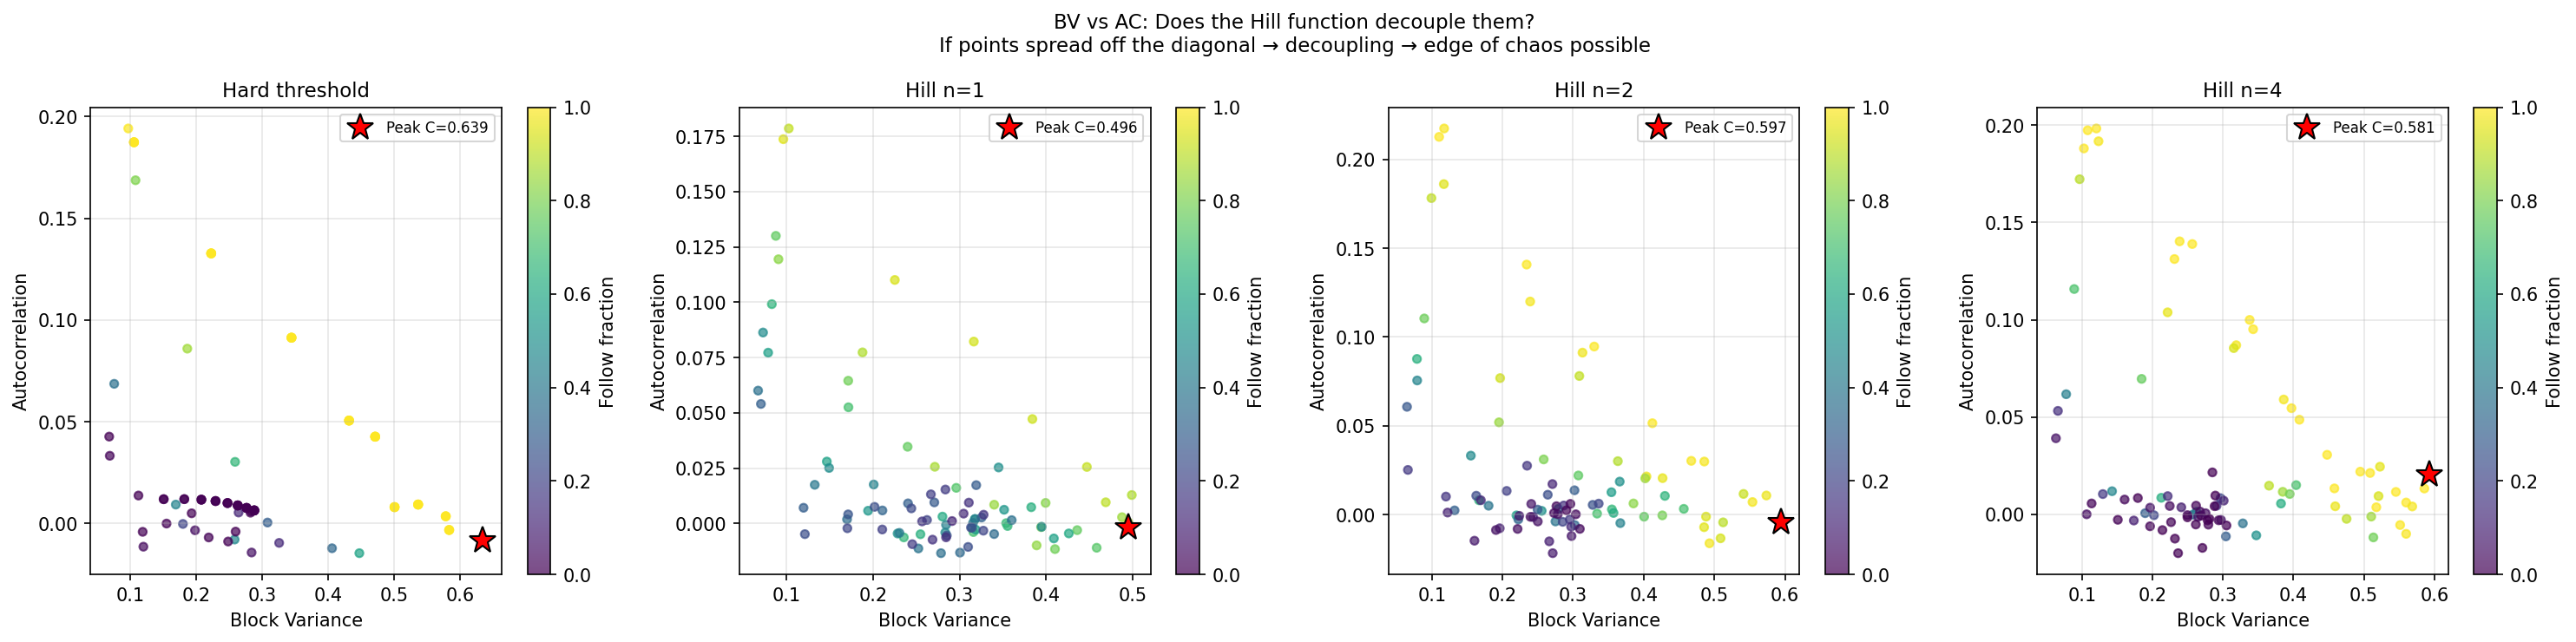
\includegraphics[width=\textwidth]{fig_study5b_scatter.png}
\caption{Block variance vs autocorrelation for each threshold type.
  All four show the same positive correlation between $B$ and $A$: state-dependent noise does not decouple them.}
\label{fig:study5b_scatter}
\end{figure}

\subsection{Why intrinsic mechanisms fail: correlated vs uncorrelated noise}

The failure of all three mechanisms reveals a structural constraint.
The composite $C = B \times (1 - A)$ peaks when trails are \emph{maximally structured yet maximally transient}---$B$ must stay high while $A$ drops.
This requires a source of disorder that is \textbf{uncorrelated with the pheromone field}.

\textbf{External noise} ($\varepsilon$) is uncorrelated: any ant, regardless of its position relative to trails, can be randomly displaced.
Strong trails lose followers at the same rate as weak trails.
This creates turnover (reducing $A$) without specifically targeting the trails that sustain structure (preserving $B$).

\textbf{Evaporation} ($\lambda$) is similarly uncorrelated with ant behaviour: it decays the pheromone field uniformly, shifting the spatial configuration while leaving the number of followers (and thus trail strength) unchanged.

All three intrinsic mechanisms produce noise that is \textbf{correlated with the pheromone field}:
\begin{itemize}
  \item \textbf{Habituation} removes ants from trails they have followed longest---precisely the strongest trails.
    This preferentially weakens the structures that contribute most to $B$.
  \item \textbf{Peaked response} redistributes ants away from the strongest trails toward weaker ones, diluting the spatial heterogeneity that $B$ measures.
  \item \textbf{Hill function} creates state-dependent noise where weak trails are followed unreliably---but weak trails are the ones that \emph{need} following to survive.
    The noise acts precisely where it destroys the most structure.
    At $n = 1$, the follow fraction smoothly interpolates from high (strong trails) to low (weak trails), but $B$ and $A$ still decline together because the noise-structure correlation is preserved.
\end{itemize}

In each case, the intrinsic noise is stronger where the pheromone signal is weaker, creating a positive feedback loop: weak trails suffer more noise $\to$ trails weaken further $\to$ more noise.
This is the opposite of what edge of chaos requires.
The composite needs a disorder source that occasionally disrupts \emph{strong} trails (reducing $A$) while the system's positive feedback rebuilds structure elsewhere (maintaining $B$).
Only uncorrelated noise---external randomness or environmental decay---achieves this.

This explains why the original noise model's edge-of-chaos ridge appeared to be intrinsic: the noise parameter $\varepsilon$ acts \emph{uniformly} on all ants regardless of their pheromone environment, making it functionally equivalent to an uncorrelated environmental perturbation rather than a state-dependent behavioural mechanism.

% ================================================================
\section{Discussion}
% ================================================================

Of nine model variants tested, only two produce edge of chaos---the original noise model and the susceptibility model---and both rely on uniform pheromone decay.
The five studies reveal two principal results: (1) sharp phase transitions and edge-of-chaos dynamics are distinct phenomena, and (2) edge of chaos is the natural outcome of uniform decay in a stigmergic system with positive feedback.

The susceptibility model decouples two axes of order that the original noise parameter conflated.
\textbf{Recruitment} (controlled by $s$) determines whether ants follow trails at all---the transition is sharp (first-order-like) but $B$ and $A$ decline together, producing no composite peak.
\textbf{Persistence} (controlled by $\lambda$) determines whether trails, once formed, survive---increasing evaporation takes the system from frozen trails through transient dynamics (peak $C$) to dissolution, a genuine edge-of-chaos trajectory.
The original noise parameter $\varepsilon$ traverses both axes simultaneously, which is why it produces a single clean ridge.

The susceptibility model is the most biologically realistic variant: pheromone deposition is unconditional (biochemical secretion), trail following is triggered by local concentration (olfactory detection), and the resulting phase transition emerges from collective dynamics rather than being imposed by a control parameter.
But the sharp recruitment boundary is not edge of chaos.
The genuine edge of chaos lies in erosion-driven transience, where environmental decay---not ant behaviour---provides the disorder.

\subsection{Unconditional deposition as nucleation noise}

A revealing test of the uncorrelated noise requirement is to \emph{couple} deposition to following: only trail-following ants deposit pheromone; asocial ants contribute nothing to the field (Figure~\ref{fig:study6}).
This creates an absorbing state---if no ant is following, no pheromone is deposited, no ant can cross threshold, and the system is permanently dead.
We initialise with pheromone $\phi_0 = 3s$ to bootstrap trail formation and sweep $s \times \lambda$.

The coupled model shows a sharp alive/dead boundary: at low $s$ ($\leq 2$), all ants follow and the model behaves identically to uncoupled; at high $s$ ($\geq 10$), the system collapses to the absorbing state.
Near the boundary ($s \approx 3$--$7$), activity concentrates into a few surviving trail fragments---block variance spikes to $B = 16.7$ at $(s = 4, \lambda = 0.20)$ with only 6\% of ants following---but this is extinction dynamics, not edge of chaos.

\begin{figure}[H]
\centering
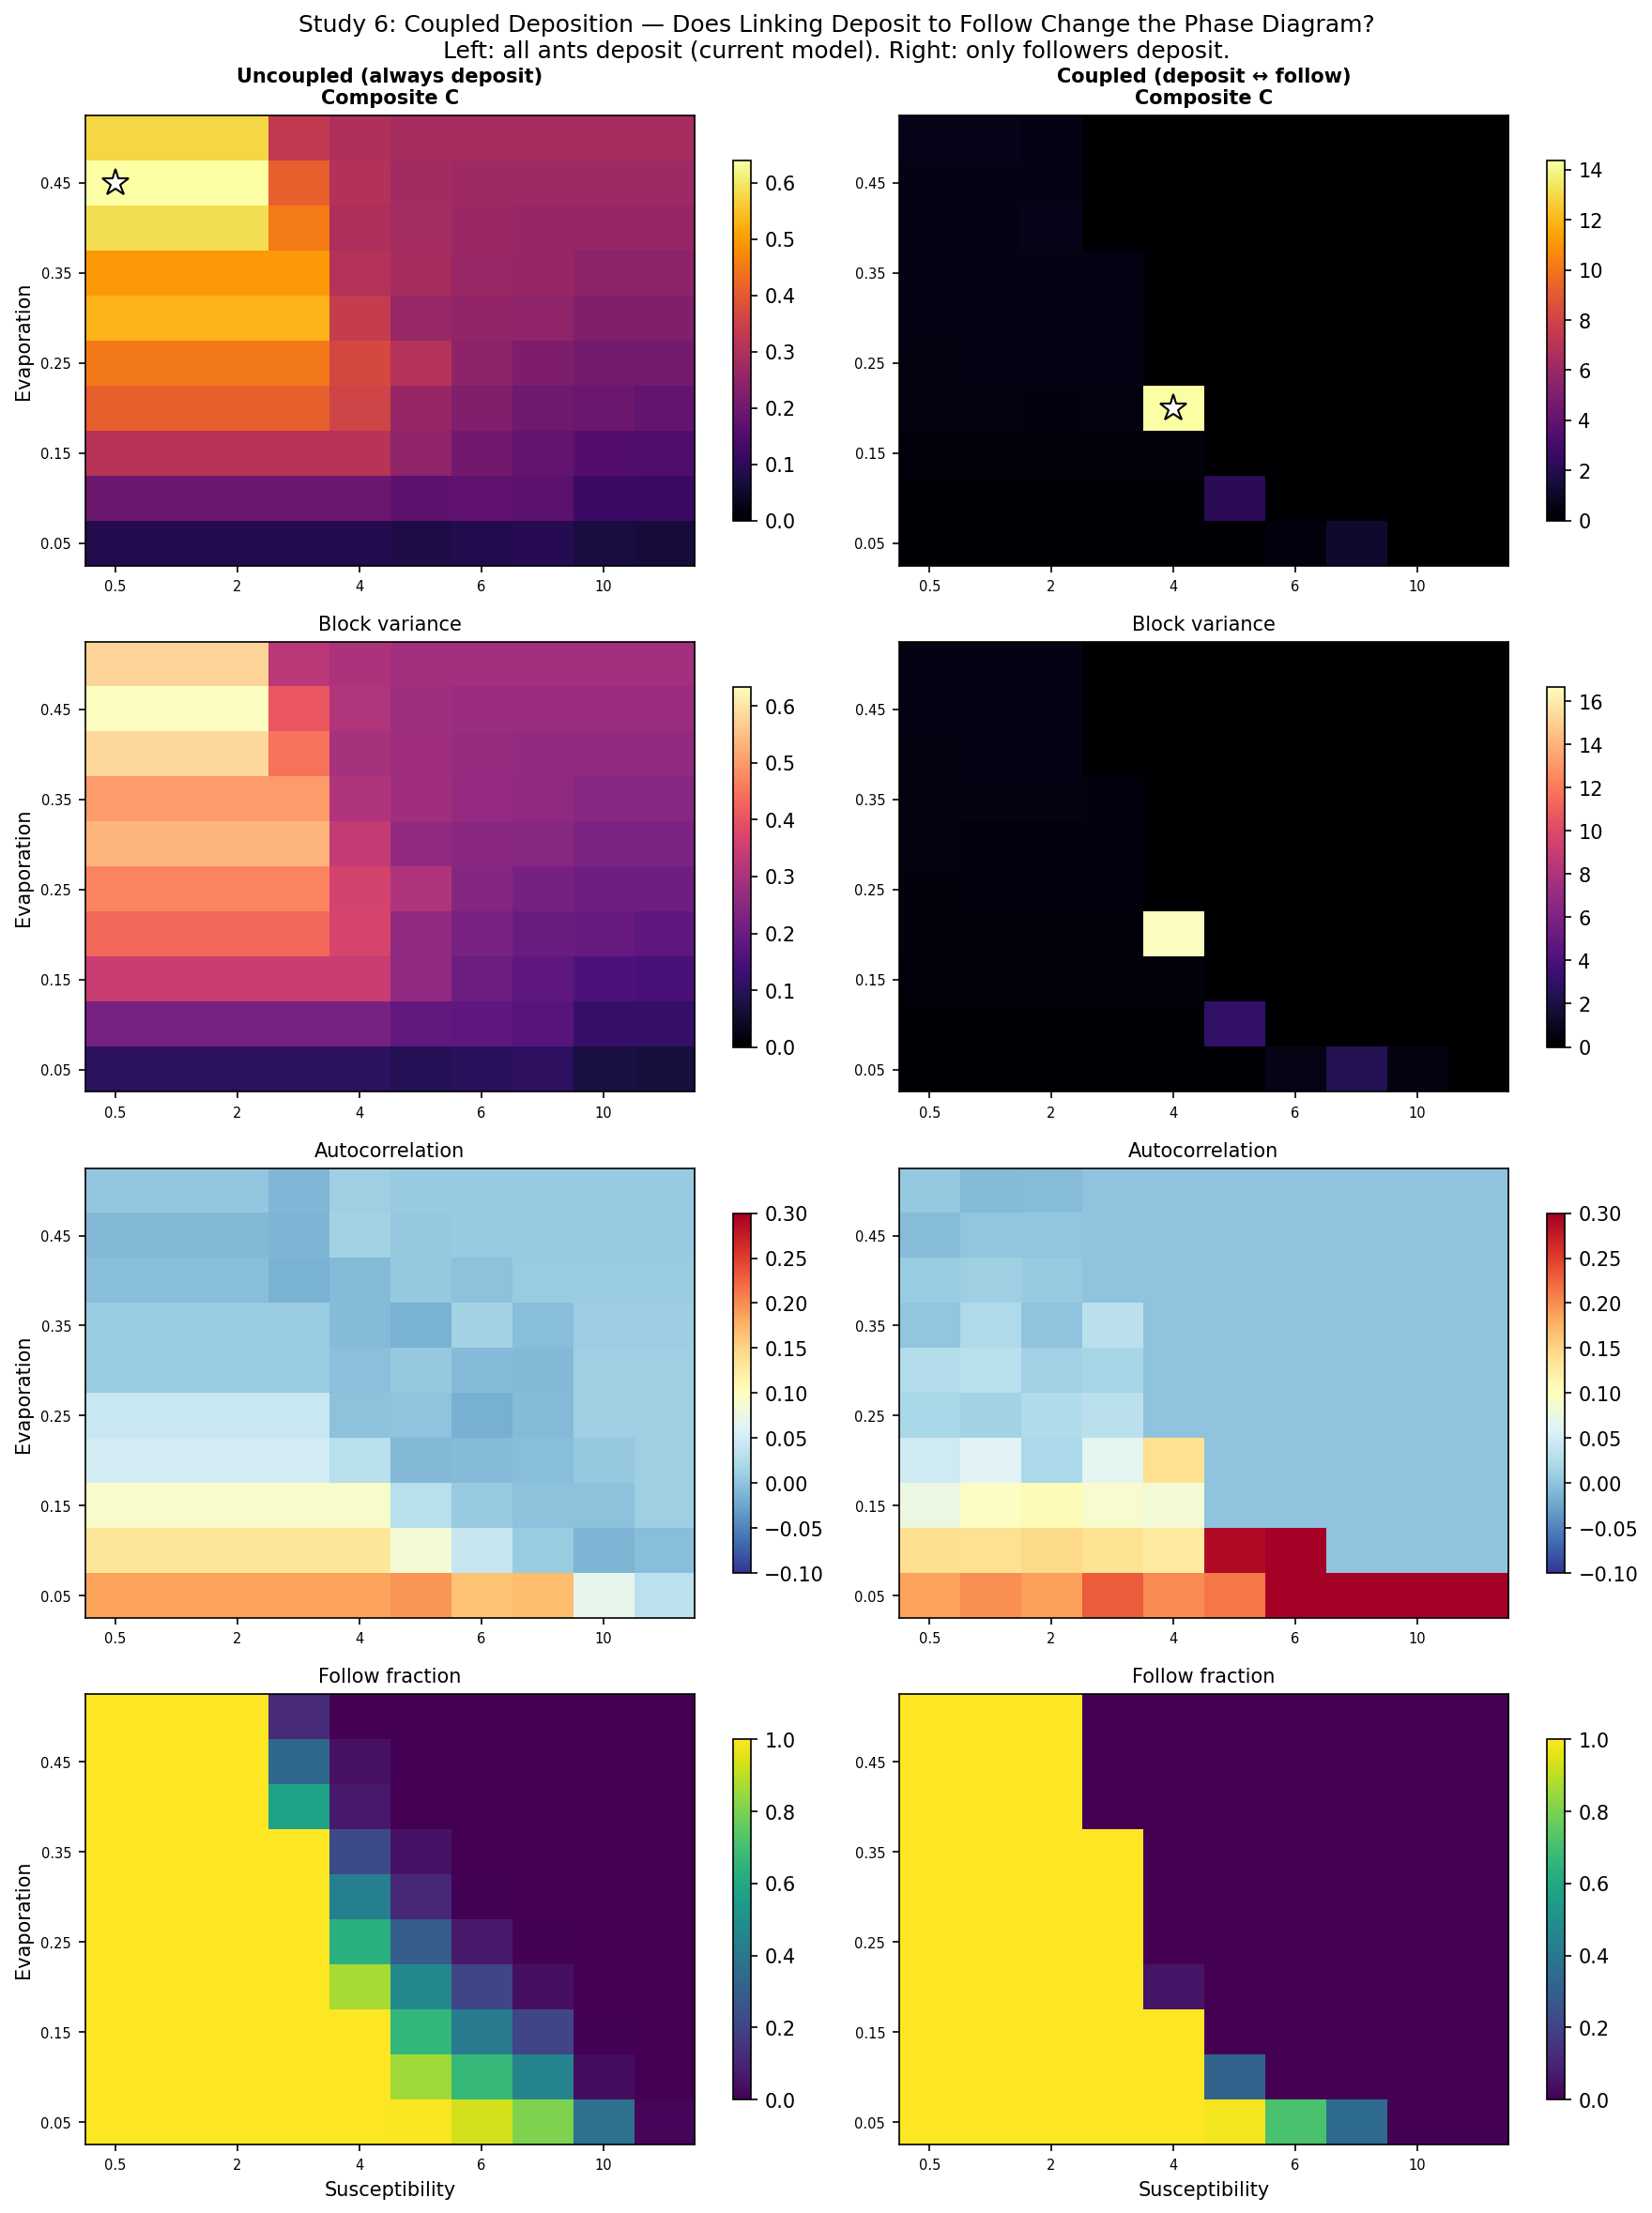
\includegraphics[width=0.98\textwidth]{fig_study6_heatmaps.png}
\caption{Coupled (right) vs uncoupled (left) deposition.
The coupled model shows a sharp alive/dead boundary (bottom row).
Extreme block variance at the boundary reflects dying clusters, not edge of chaos.}
\label{fig:study6}
\end{figure}

The implication is that unconditional deposition---random-walking ants laying pheromone regardless of their following state---is itself a form of uncorrelated noise.
It provides a nucleation floor from which trails can spontaneously form, independent of the current collective state.
Remove it and the system has no escape from the absorbing state.
This connects to the broader theory of absorbing state phase transitions: in epidemiological models, spontaneous infection prevents disease extinction; in catalytic reactions, external particle injection maintains activity.
In each case, a source of activity uncorrelated with the current state is required.
In our model, unconditional deposition plays exactly this role---a third source of uncorrelated noise alongside $\varepsilon$ and $\lambda$ that was present all along but invisible because it was never varied.

\subsection{Relation to noise correlation theory}

Our finding---that edge of chaos requires disorder uncorrelated with the collective signal---is an instance of a broader principle in the theory of multiplicative noise and critical phenomena.

\textbf{Multiplicative vs additive noise.}
Horsthemke \& Lefever (1984) established that multiplicative noise (state-dependent, intensity varying with the order parameter) qualitatively reshapes the effective potential landscape, while additive noise (state-independent) merely broadens distributions around existing attractors.
Our intrinsic mechanisms---susceptibility threshold, Hill function, habituation---are multiplicative: the noise intensity depends on pheromone concentration.
External noise $\varepsilon$ and evaporation $\lambda$ are additive: they act uniformly regardless of the field state.
Grinstein, Mu\~noz \& Tu (1996) showed that multiplicative noise can eliminate critical points that exist under additive noise, and Mu\~noz and collaborators demonstrated that it generically changes the universality class of absorbing-state phase transitions.
Van den Broeck, Parrondo \& Toral (1994) showed that multiplicative noise can induce its \emph{own} phase transitions, but in different universality classes---consistent with our observation that intrinsic mechanisms produce sharp recruitment transitions but not the edge-of-chaos ridge.

\textbf{Self-organised criticality.}
In SOC models (Bak, Tang \& Wiesenfeld, 1987), the slow driving is deliberately uncorrelated with the system state---grains are dropped at random locations regardless of local height.
Hwa \& Kardar (1989) showed that state-dependent driving disrupts SOC.
Vespignani \& Zapperi (1998) provided a mean-field framework showing that SOC requires driving that is ``uninformed'' about the system state.
Our pheromone model is not SOC (it lacks separation of timescales), but the same principle applies: the disorder source must be decoupled from the order parameter.

\textbf{Flocking models.}
The closest parallel to our result comes from the Vicsek model of collective motion.
Aldana et al.\ (2007) and Chat\'e et al.\ (2008) showed that \emph{intrinsic angular noise} (uncorrelated with local alignment) produces a continuous order--disorder phase transition with a true critical point, while \emph{vectorial noise} (correlated with the local order parameter) makes the transition discontinuous---the system jumps over the critical point entirely.
This maps directly onto our finding: uncorrelated noise sustains the edge of chaos; correlated noise produces a first-order collapse.
The Vicsek model's alignment field plays the role of our pheromone field, and the noise correlation structure determines whether the transition is continuous (edge of chaos) or discontinuous (first-order collapse).

\textbf{Neural criticality.}
Bonachela, Torres \& Mu\~noz (2010) showed that synaptic depression---a state-dependent negative feedback mechanism where synapses weaken in proportion to recent activity---produces only \emph{quasi-critical} behaviour in neural networks, not true criticality.
True criticality requires background synaptic noise: uncorrelated spontaneous vesicle release and channel noise.
Shew \& Plenz (2013) confirmed that homeostatic mechanisms (correlated feedback) produce oscillation around the critical point, while uncorrelated fluctuations stabilise it.
Synaptic depression is structurally analogous to our habituation mechanism: both are state-dependent negative feedback that fails to sustain criticality because the noise is correlated with the activity it aims to regulate.

These results across flocking, neural, and SOC systems suggest that the principle we identify---edge of chaos requires uncorrelated noise---is not specific to stigmergic trail systems but reflects a general constraint on criticality in systems with positive feedback.

% ================================================================
\section{Summary}
% ================================================================

\begin{table}[H]
\centering
\caption{Summary of all parameter sweeps. ``EoC ridge'' indicates whether the composite order parameter forms a sharp peak (edge-of-chaos ridge), distinct from whether the model has a sharp phase transition in follow fraction.}
\label{tab:summary}
\small
\begin{tabular}{@{}llcccp{3.2cm}@{}}
\toprule
Model & Sweep axes & Struct. metric & Peak $C$ & EoC ridge? & Mechanism \\
\midrule
Original & $\varepsilon \times \lambda$ & Linearity & 0.312 & Yes & Coupled destruction \\
Simple ($\mu{=}3$) & $p_f \times \lambda$ & Linearity & 0.309 & No & Decoupled control \\
Simple ($\mu{=}0.5$) & $p_f \times \lambda$ & Linearity & 0.287 & No & Decoupled control \\
Simple (3D) & $p_f {\times} \lambda {\times} \sigma$ & Linearity & 0.300 & No & Decoupled control \\
\textbf{Suscept. (v2)} & $\boldsymbol{s {\times} \lambda {\times} \sigma}$ & \textbf{Block var.} & \textbf{0.625} & \textbf{Yes}$^\dagger$ & \textbf{Erosion-driven} \\
Suscept. ($C_R$) & $s {\times} \lambda {\times} \sigma$ & Block var. $\times\, 4f(1{-}f)$ & 0.484 & No$^\ddagger$ & Recruitment collapse \\
Habituation & $\tau_h \times \lambda$ & Block var. & 0.678$^\S$ & No & Correlated neg. feedback \\
Peaked resp. & $\phi_\text{sat} \times \lambda$ & Block var. & 0.639$^\S$ & No & Correlated redistribution \\
Hill ($n{=}2$) & $s \times \lambda$ & Block var. & 0.597$^\S$ & No & Correlated state-dep. noise \\
\bottomrule
\multicolumn{6}{@{}l}{\footnotesize $^\dagger$Along persistence axis (evaporation), not at recruitment boundary.} \\
\multicolumn{6}{@{}l}{\footnotesize $^\ddagger$Sharp phase transition in $f$, but composite drops monotonically---not edge of chaos.} \\
\multicolumn{6}{@{}l}{\footnotesize $^\S$Peak at boundary of swept range---no interior peak in the intrinsic parameter.}
\end{tabular}
\end{table}

Of nine model variants tested, \textbf{only two produced edge of chaos} (Table~\ref{tab:summary}).
Both share the same essential ingredient: \textbf{uniform pheromone decay}.

The \textbf{original model} ($\varepsilon \times \lambda$) produces an edge-of-chaos ridge ($C = 0.312$).
The \textbf{susceptibility model} produces a stronger one ($C = 0.625$), but \emph{only along the evaporation axis}---the susceptibility axis produces a sharp recruitment transition that is not edge of chaos.
No other model variant---the simple model (three variants), habituation, peaked response, Hill function, or coupled deposition---produces an edge-of-chaos ridge.

The susceptibility model is the more revealing of the two positive cases.
It contains no external noise parameter at all: ants deposit pheromone unconditionally, follow trails above a concentration threshold, and the pheromone field decays uniformly.
Edge of chaos emerges from just three elements: \textbf{localised deposition} (ants deposit where they walk), \textbf{positive feedback} (following concentrates ants on trails), and \textbf{uniform decay} (evaporation erodes all pheromone equally).
The balance between trail formation and trail erosion naturally creates a regime of transient, spatially heterogeneous dynamics---the edge of chaos.

The seven negative cases all attempted to replace uniform decay with a state-dependent mechanism.
Every attempt failed because state-dependent disorder is correlated with the pheromone field:

\begin{itemize}
  \item \textbf{Habituation} targets ants on the strongest trails, preferentially weakening the structures that contribute most to spatial heterogeneity.
  \item \textbf{Peaked response} redistributes ants away from strong trails, diluting concentration.
  \item \textbf{Hill function} makes weak trails unreliable, destroying the structures that most need reinforcement.
  \item \textbf{Coupled deposition} removes the nucleation floor from non-following ants, creating an absorbing state.
\end{itemize}

In each case, the disorder source is stronger where the pheromone signal is weaker, creating a positive feedback loop toward collapse: weak trails suffer more noise, weaken further, suffer more noise.
Edge of chaos requires the opposite: disorder that occasionally disrupts \emph{strong} trails (reducing persistence $A$) while positive feedback rebuilds structure elsewhere (maintaining heterogeneity $B$).
Only uniform decay achieves this, because it erodes all trails equally regardless of their strength.

\begin{quote}
\textbf{Edge of chaos is the default in stigmergic systems with uniform decay.
The hard problem is not producing it---it is not destroying it.}
\end{quote}

The original model's noise parameter $\varepsilon$ succeeds for the same reason as evaporation: it acts uniformly on all ants regardless of what they smell.
An ant that moves randomly with probability $\varepsilon$ is functionally equivalent to an environmental perturbation---it disrupts strong and weak trails with equal probability.
The susceptibility model shows that $\varepsilon$ is not necessary: uniform decay alone is sufficient.
The minimal system is simply ants that deposit, ants that follow concentrations, and a field that decays.

% ================================================================
\appendix
\section{Toward a Constructive Theory}
\label{app:constructive}
% ================================================================

The preceding studies are diagnostic: they identify which mechanisms fail and why.
Here we attempt to go further---to state a \emph{constructive} recipe for edge of chaos in stigmergic systems and test it by prediction.

\subsection{The recipe}

A stigmergic system has agents that read from and write to a shared field $\phi$.
Abstracting over all models tested, we identify three processes:

\begin{enumerate}
  \item \textbf{Amplification} (positive feedback).
    Agents sense the field and concentrate where $\phi$ is strong, reinforcing it.
    This process is necessarily \emph{correlated} with $\phi$---that is what makes it amplification.
  \item \textbf{Injection} (signal source).
    New signal enters the field.
    This may be correlated with $\phi$ (only followers deposit) or uncorrelated (all agents deposit regardless of state).
  \item \textbf{Erosion} (signal sink).
    Signal leaves the field.
    This may be correlated with $\phi$ (habituation targets active trails) or uncorrelated (evaporation acts uniformly).
\end{enumerate}

In mean-field terms:
\begin{equation}
  \frac{d\phi}{dt} = \underbrace{\alpha}_{\text{injection}} + \underbrace{\beta \cdot g(\phi)}_{\text{amplification}} - \underbrace{\lambda \cdot \phi}_{\text{erosion}} + D\nabla^2\phi
  \label{eq:recipe}
\end{equation}
where $\alpha$ is the unconditional injection rate, $g(\phi)$ is the amplification kernel (increasing in $\phi$), $\lambda$ is the decay rate, and $D$ is diffusion.

\textbf{The recipe}: edge of chaos requires
\begin{enumerate}
  \item[(R1)] Positive feedback ($\beta > 0$, $g(\phi)$ increasing): creates spatial structure.
  \item[(R2)] Uncorrelated injection ($\alpha > 0$, independent of $\phi$): prevents the absorbing state and provides nucleation for new structures.
  \item[(R3)] Uncorrelated erosion ($\lambda > 0$, independent of agent state): provides turnover without preferentially targeting specific structures.
\end{enumerate}
Edge of chaos is the regime where the formation timescale (set by $\alpha + \beta g$) approximately matches the erosion timescale (set by $\lambda$).

Table~\ref{tab:recipe} maps this recipe onto every model tested.

\begin{table}[H]
\centering
\caption{The three-ingredient recipe applied to all models. Each column indicates whether the ingredient is present (\checkmark), absent ($\times$), or correlated with $\phi$ ($\sim$). Edge of chaos requires all three uncorrelated.}
\label{tab:recipe}
\small
\begin{tabular}{@{}lcccc@{}}
\toprule
Model & Amplification & Injection & Erosion & EoC? \\
\midrule
Original ($\varepsilon$) & \checkmark (following) & \checkmark (unconditional dep.) & \checkmark (evaporation) & \textbf{Yes} \\
Simple ($p_f$) & weak (no threshold) & \checkmark & \checkmark & No$^a$ \\
Susceptibility ($s$) & \checkmark & \checkmark & \checkmark & \textbf{Yes}$^b$ \\
Habituation & \checkmark & \checkmark & $\sim$ (targets active) & No \\
Peaked response & \checkmark & \checkmark & $\sim$ (redistributes) & No \\
Hill function & \checkmark & \checkmark & $\sim$ (weak trails) & No \\
Coupled deposition & \checkmark & $\sim$ (only followers) & \checkmark & No$^c$ \\
No feedback (random) & $\times$ & \checkmark & \checkmark & No \\
\bottomrule
\multicolumn{5}{@{}p{11cm}@{}}{\footnotesize $^a$Momentum produces structure without threshold-based amplification; $p_f$ lacks the positive feedback loop. $^b$Along the evaporation axis only. $^c$Edge of chaos in the alive region, but absorbing state truncates the accessible parameter range.}
\end{tabular}
\end{table}

\subsection{Predictions and test}

If the recipe is correct, we can make four predictions for a minimal system (agents on a grid with a single resource field, susceptibility $s = 3$, varying evaporation $\lambda$):

\begin{enumerate}
  \item \textbf{Full recipe} (all three ingredients present): the composite $C$ will have an interior peak in $\lambda$.
  \item \textbf{Remove uncorrelated injection} (coupled deposition---only followers deposit): the system will collapse to an absorbing state at high $\lambda$, truncating or eliminating the peak.
  \item \textbf{Remove uncorrelated erosion} ($\lambda = 0$, use habituation instead): the field will freeze, $A \to 1$, and $C \approx 0$.
  \item \textbf{Remove positive feedback} (agents ignore the field, random walk): no concentrated structure will form; $B$ will rise monotonically with $\lambda$ (trivial dilution effect) with no interior peak.
\end{enumerate}

Figure~\ref{fig:constructive} shows the results.
Three of four predictions hold cleanly:
the full recipe produces an interior peak at $\lambda = 0.35$ ($C = 0.58$);
the no-erosion control is frozen ($C = 0.001$);
the no-feedback control rises monotonically with no peak.

The coupled deposition control (prediction 2) reveals a refinement: the system \emph{does} show edge-of-chaos dynamics in the alive region ($\lambda < 0.39$), tracking the full recipe almost exactly, before collapsing to the absorbing state.
This is because at low $\lambda$, all ants follow ($f = 1.0$) and all deposit, making injection effectively uncorrelated.
The absorbing state only matters when some ants stop following---then the loss of their deposition creates a positive feedback toward extinction.
This separates two roles of uncorrelated injection: (i)~sustaining transient dynamics (shared with erosion) and (ii)~preventing the absorbing state (a distinct existential requirement).

\begin{figure}[H]
\centering
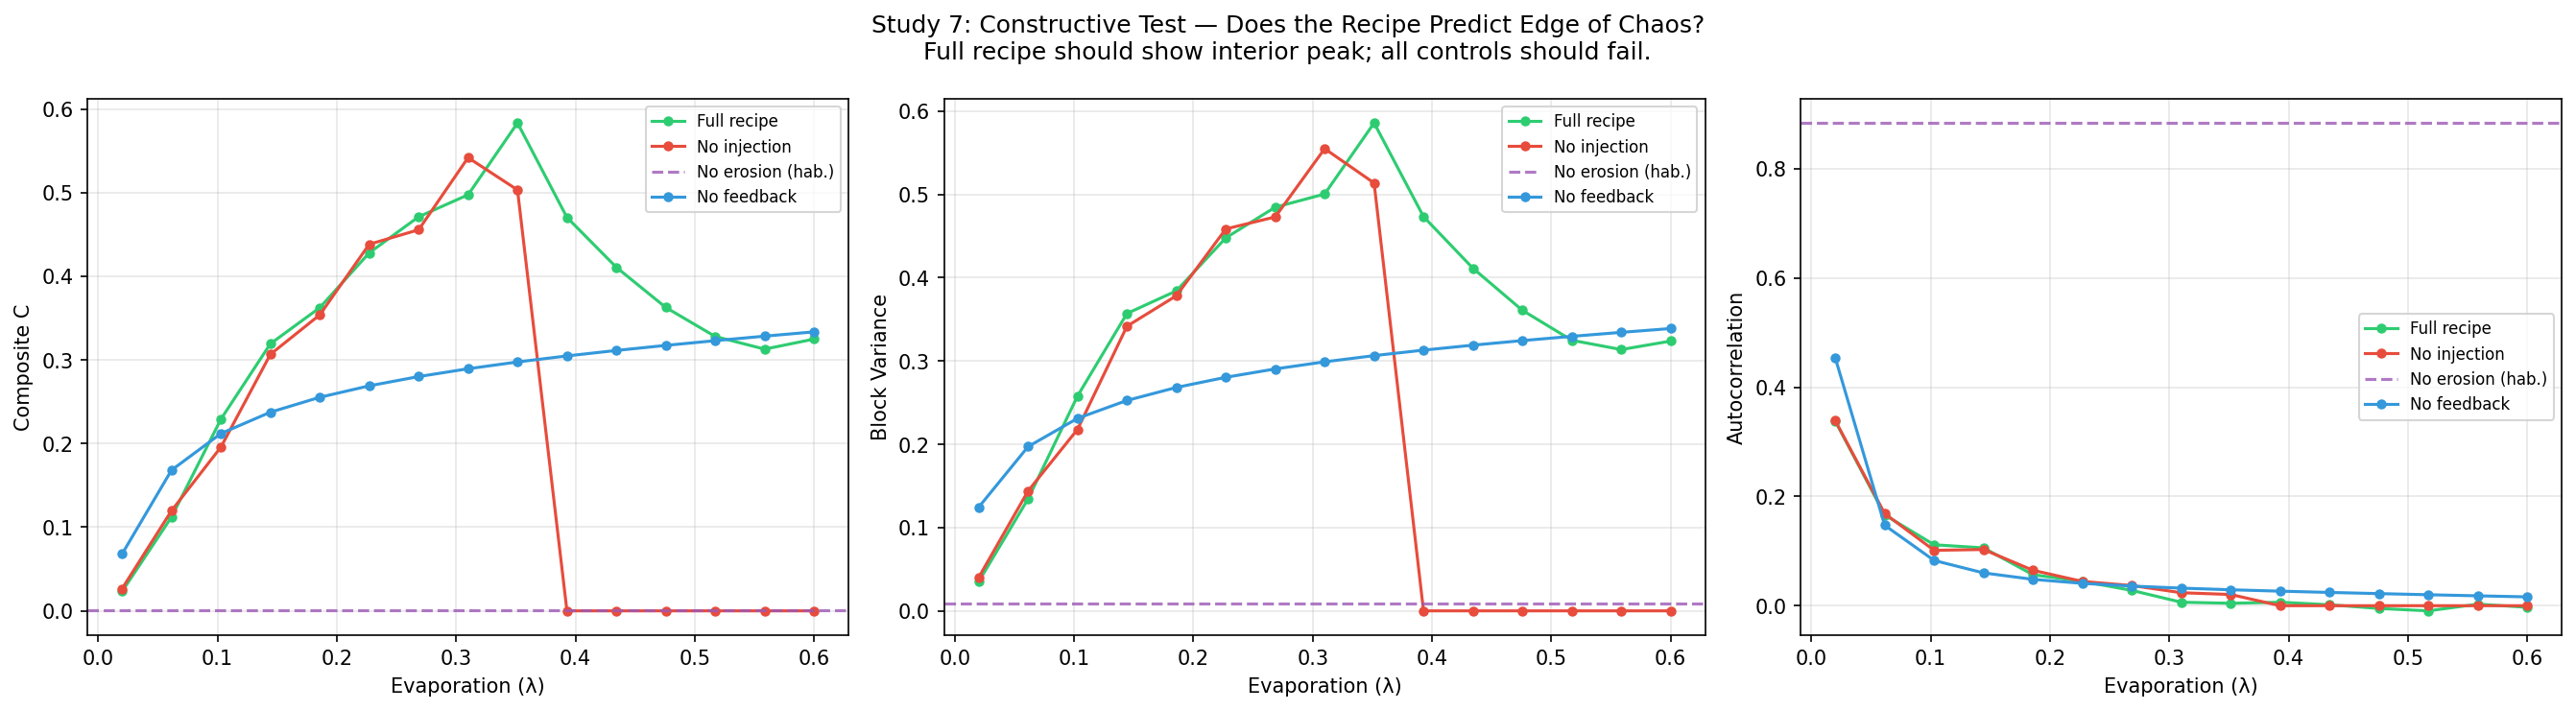
\includegraphics[width=0.98\textwidth]{study7_constructive.png}
\caption{Constructive test of the three-ingredient recipe.
Green: full recipe (interior peak at $\lambda = 0.35$, confirming edge of chaos).
Red: coupled deposition (tracks full recipe until absorbing state kills it at $\lambda \geq 0.39$).
Purple dashed: habituation with no decay (frozen, $C \approx 0$).
Blue: no positive feedback (monotonic rise, no peak).
Three of four predictions confirmed; the fourth reveals a refinement about the absorbing state.}
\label{fig:constructive}
\end{figure}

\subsection{From description to prediction}

The recipe provides a checklist for any candidate stigmergic system:

\begin{enumerate}
  \item \textbf{Identify the shared field} ($\phi$)---the medium through which agents interact indirectly.
  \item \textbf{Check for positive feedback}: do agents amplify $\phi$ where it is already strong?  If not, no spatial structure will form.
  \item \textbf{Check injection}: is there a source of $\phi$ that operates independently of the current field state?  If injection depends on $\phi$ (e.g., only active agents contribute), the system risks an absorbing state.
  \item \textbf{Check erosion}: is there a sink that removes $\phi$ independently of agent state?  If erosion depends on $\phi$ (e.g., targeting the strongest concentrations), it will produce first-order collapse rather than gradual turnover.
  \item \textbf{Find the balance point}: vary the erosion rate.  If injection $+$ amplification can balance erosion, an edge-of-chaos regime should exist at the balance point.
\end{enumerate}

This checklist is not specific to ant pheromone systems.
It should apply to any system where agents read from and write to a shared persistent medium---including, potentially, market microstructure (price as $\phi$, buying/selling as injection, information decay as erosion), urban growth (infrastructure as $\phi$, investment as injection, depreciation as erosion), or neural ensembles (synaptic weight as $\phi$, Hebbian learning as amplification, synaptic decay as erosion).

The key constraint is that edge of chaos requires the disorder sources to be \emph{structurally uncorrelated} with the order parameter.
Any system where both injection and erosion act independently of the current field, with positive feedback in between, is a candidate.

\end{document}
